\documentclass[aspectratio=169,11pt,usenames,dvipsnames]{beamer}

% \usepackage[colorlinks=true,linkcolor=customblue, citecolor=hpred,urlcolor=customlightblue]{hyperref}

\usetheme{simple}

% packages
\usepackage{mathrsfs}  
\usepackage{cancel}
% \usepackage{caption}
% \usepackage{tikz}

\makeatother
\renewcommand{\thefootnote}{\color{customblue}\faPaperPlaneO}
\makeatletter

\newcommand{\symfootnote}[1]{%
\let\oldthefootnote=\thefootnote%
\stepcounter{mpfootnote}%
\addtocounter{footnote}{-1}%
\renewcommand{\thefootnote}{$\dagger$}%
\footnote{#1}%
\let\thefootnote=\oldthefootnote%
}

\newcommand\blfootnote[1]{%
  \begingroup
  \renewcommand\thefootnote{}\footnote{#1}%
  \addtocounter{footnote}{-1}%
  \endgroup
}

\usepackage{xcolor}
\usepackage{graphicx}
\usepackage{empheq}
\usepackage{physics}
\usepackage{svg}
\usepackage{bm}
\usepackage{amsmath}
\usepackage{amssymb}
\usepackage{annotate-equations}

\usepackage{appendixnumberbeamer}

\usepackage{relsize}

\usepackage{fontawesome}


\usetikzlibrary{decorations.pathreplacing, decorations.pathmorphing,calc,arrows,positioning}

% Custom colors

\definecolor{isred}{HTML}{81182d}
\definecolor{hpred}{HTML}{712A27}
\definecolor{hpblue}{HTML}{44545c}

\definecolor{customblue}{HTML}{3c9bb3}
\definecolor{customgreen}{HTML}{117877}
\definecolor{custompink}{HTML}{c35861}
\definecolor{customred}{HTML}{9d1700}
\definecolor{customyellow}{HTML}{e0ad04}
\definecolor{lightgray}{HTML}{a6a4a4}

\definecolor{lightcustomblue}{HTML}{aad1e6}
\definecolor{lightpink}{HTML}{ba8489}

\definecolor{starrymain}{HTML}{3B5B65}
\definecolor{starrysecond}{HTML}{719593}

\definecolor{ektgreen}{HTML}{047c73}
\definecolor{ektblue}{HTML}{065680}

\definecolor{angcorr}{HTML}{502d7e}

\definecolor{pinky}{HTML}{c35861}
\definecolor{ming}{HTML}{117877}

\definecolor{jyublue}{HTML}{002145}
\definecolor{jyured}{HTML}{e13126}
\definecolor{jyulightblue}{HTML}{909eae}

\definecolor{paldarkblue}{HTML}{0d1f2d}
\definecolor{pallightblue}{HTML}{2f586e}
\definecolor{paldarkgold}{HTML}{d2973b}
\definecolor{pallightgold}{HTML}{e8ca84}
\definecolor{palred}{HTML}{8c0e0f}

\definecolor{palblue}{HTML}{0d3672}
\definecolor{palteal}{HTML}{406f6b}
\definecolor{palgold}{HTML}{b99146}
\definecolor{palviolet}{HTML}{9F87AF}

\definecolor{raapink}{HTML}{ce93b5}
\definecolor{raablue}{HTML}{5c93b8}

\usepackage{etoolbox}
\setbeamertemplate{blocks}[rounded][shadow=false]
\setbeamercolor{block title}{use=structure,fg=palteal,bg=palteal!10}
\setbeamercolor{block body}{parent=normal text,use=block title,bg=palteal!10}

\usepackage[most]{tcolorbox}
\newtcolorbox{mybox}[2][]{tcbox width=auto limited,capture=hbox,colbacktitle=red!10!white, colback=blue!10!white,coltitle=red!70!black, title={#2},fonttitle=\bfseries,#1}

\newtcolorbox{custombox}[3][]{%
    enhanced jigsaw,%
    colback=#3!5,%
    colframe=#3,%
    colbacktitle=#3!5,
    coltext=normal,
    center title,
    % size=small,%
    hbox,%
    center title,%
    % boxrule=1pt,%
    % title=\textbf{\textit{Example}},%
    % halign title=flush left,%
    coltitle=#3,%
    breakable,%
    boxrule=1.1pt,
    titlerule=0pt,
    left=-3pt,
    right=-3pt,
    top=2pt,
    bottom=0pt,
    enlarge left by=-0.1cm,
    grow to right by=0.21cm,
    title={#2},fonttitle=\bfseries\large,#1
}
\newtcolorbox{custombox2}[3][]{%
    enhanced jigsaw,%
    colback=#3!10,%
    colframe=#3,%
    colbacktitle=#3!10,
    coltext=normal,
    center title,
    % size=small,%
    hbox,%
    center title,%
    % boxrule=1pt,%
    % title=\textbf{\textit{Example}},%
    % halign title=flush left,%
    coltitle=#3,%
    breakable,%
    boxrule=0pt,
    titlerule=0pt,
    left=-8pt,
    right=-8pt,
    top=2pt,
    bottom=0pt,
    enlarge left by=-0.1cm,
    grow to right by=0.21cm,
    title={#2},fonttitle=\bfseries\large,#1
}
\newtcolorbox{custombox2transp}[3][]{%
    enhanced jigsaw,%
    colback=#3!4,%
    colframe=#3,%
    colbacktitle=#3!4,
    coltext=normal,
    center title,
    % size=small,%
    hbox,%
    center title,%
    % boxrule=1pt,%
    % title=\textbf{\textit{Example}},%
    % halign title=flush left,%
    coltitle=#3,%
    breakable,%
    boxrule=0pt,
    titlerule=0pt,
    left=-8pt,
    right=-8pt,
    top=2pt,
    bottom=0pt,
    enlarge left by=-0.1cm,
    grow to right by=0.21cm,
    title={#2},fonttitle=\bfseries\large,#1
}
\newtcolorbox{untitledcustombox}{%
    enhanced jigsaw,%
    colback=palteal!10,%
    colframe=palteal,%
    % colbacktitle=#1!10,
    coltext=normal,
    % center title,
    % size=small,%
    hbox,%
    center title,%
    % boxrule=1pt,%
    % title=\textbf{\textit{Example}},%
    % halign title=flush left,%
    % coltitle=#1,%
    breakable,%
    boxrule=0pt,
    titlerule=0pt,
    left=-2pt,
    right=-2pt,
    top=2pt,
    bottom=1pt,
    enlarge left by=-0.1cm,
    grow to right by=0.21cm,
}
\newtcolorbox{untitledcustomboxtransp}{%
    enhanced jigsaw,%
    colback=palteal!4,%
    colframe=palteal,%
    % colbacktitle=#1!10,
    coltext=normal,
    % center title,
    % size=small,%
    hbox,%
    center title,%
    % boxrule=1pt,%
    % title=\textbf{\textit{Example}},%
    % halign title=flush left,%
    % coltitle=#1,%
    breakable,%
    boxrule=0pt,
    titlerule=0pt,
    left=-2pt,
    right=-2pt,
    top=2pt,
    bottom=1pt,
    enlarge left by=-0.1cm,
    grow to right by=0.21cm,
}
\usepackage{varwidth}

\hypersetup{colorlinks,linkcolor=normal,citecolor=customblue, citecolor=pinky,urlcolor=pinky}

% custom commands
\newcommand{\coloredeq}[2]{\begin{empheq}[box=\colorbox{#1}]{align*}#2\end{empheq}}
\newcommand\scalemath[2]{\scalebox{#1}{\mbox{\ensuremath{\displaystyle #2}}}}
\newcommand\coloreditem[1]{\item[\textcolor{#1}{\usebeamertemplate{itemize \beameritemnestingprefix item}}]}
\newcommand{\imp}[1]{{\sffamily\bfseries\color{customblue}#1}}

\setbeamertemplate{frametitle}[default][center]

\usepackage{etoolbox}% http://ctan.org/pkg/etoolbox
\makeatletter
\newlength{\secnamelength}
\newsavebox{\longestsec}% Box to save longest sectional heading
\patchcmd{\beamer@section}% <cmd>
  {\beamer@savemode}% <search>
  {\begin{lrbox}{\longestsec}#1\end{lrbox}%
   \ifdim\wd\longestsec>\secnamelength\relax\setlength{\secnamelength}{\wd\longestsec}\fi%
   \beamer@savemode}% <replace>
  {}{}% <success><failure>
\AtEndDocument{% http://tex.stackexchange.com/q/137495/5764
  \immediate\write\@auxout{\global\secnamelength=\the\secnamelength}%
}
\makeatother


\renewcommand{\d}{\mathrm{d}}
\renewcommand{\tr}[1]{\mathrm{Tr}\left\{#1\right\}}

\usepackage{scalerel}
\newcommand\Blacktriangleright{\raisebox{0.2em}{\scaleobj{0.7}{\blacktriangleright}}}

% customize beamer
% \setbeamercolor{frametitle}{fg=jyublue}
\setbeamercolor{framesubtitle}{fg=normal}
\setbeamercolor{subtitle}{fg=customblue}
% \setbeamerfont{frametitle}{series=\normalfont\huge}
\setbeamerfont{frametitle}{series=\normalfont\huge}
\setbeamerfont{framesubtitle}{series=\normalfont\normalsize}
\setbeamerfont{section in toc}{series=\normalfont\Large}
% \setbeamercolor{section in toc}{fg=red}
\setbeamerfont{subsection in toc}{series=\normalfont\small}
% \setbeamerfont{subsection in toc}{series=\itshape}

% all subsections in TOC in a single line
\defbeamertemplate*{subsection in toc}{sub on 1 line}
{
  \ifnum\inserttocsubsectionnumber=1
    \vspace{0.1cm}\hspace{0.45cm}\inserttocsubsection
  \else
    {\color{normal}$\sbullet[0.6]$}\hspace{0.2cm}\inserttocsubsection
  \fi
}


\usefonttheme[onlymath]{serif}

% Item shape and color
\setbeamertemplate{itemize item}{\raisebox{0.2em}{\scalebox{0.7}{${\color{customblue}\blacktriangleright}$}}} 

\newcommand{\itemcolor}[1]{\setbeamertemplate{itemize item}{\raisebox{0.2em}{\scalebox{0.7}{${\color{#1}\blacktriangleright}$}}}}
\addtobeamertemplate{navigation symbols}{}{%
    \usebeamerfont{footline}%
    \usebeamercolor[fg]{footline}%
    \hspace{1em}%
    \insertframenumber/\inserttotalframenumber
}
\setbeamercolor{footline}{fg=customblue}
\setbeamerfont{footline}{series=\normalfont\footnotesize}
\setbeamertemplate{navigation symbols}{}

% scale bullet symbol
\newcommand\sbullet[1][.5]{\mathbin{\vcenter{\hbox{\scalebox{#1}{$\bullet$}}}}}

% colored box environment
\usepackage{tcolorbox}
\tcbuselibrary{skins,hooks}
\newcommand\fancybox[3]{%
\tcbset{
    mybox/.style={
        enhanced,
        boxsep=0mm,
        opacityfill=0,
        overlay={
            \coordinate (X) at ([xshift=2mm, yshift=-1.5mm]frame.north east);
            \node[align=left, text=#1, text width=5cm, anchor=north west] at (X) {#2};
            \draw[line width=0.3mm, color=#1] (frame.north east) -- (frame.south east); 
            }
        }
    }

\begin{tcolorbox}[mybox]
    #3
\end{tcolorbox}
}

% figure caption
\usepackage{caption}
\captionsetup[figure]{labelformat=empty}

% title page
\title{\normalfont\bfseries\Large Transport of {\color{jyublue}jets} and {\color{jyublue}heavy quarks} in the\\
 {\color{jyured}glasma} pre-equilibrium stage\vspace{-10pt}}
\date{\vspace{-20pt}
    \begin{center}
        \resizebox{.9\textwidth}{!}{%
        
\includegraphics[height=0.7cm]{images/university-of-jyvaskyla-logo-freelogovectors.net_.png}%
        \quad
        
\includegraphics[height=0.7cm]{images/HIP_Logo_EN_V4_Pos_Blue.pdf}%
        \quad
        
\includegraphics[height=0.75cm]{images/CoE-logo-01_nobg.png}%
        \quad
        
\includegraphics[height=0.8cm]{images/AKA_EN_pysty_sininen_RGB.png}%
        \quad
        
\includegraphics[height=0.7cm]{images/Logo-ERC-black_0.png}%
        }
    \end{center}

    \begin{columns}
        \begin{column}{0.1\textwidth}\end{column}
        \begin{column}{0.8\textwidth}
            \centering
            \footnotesize High energy probes of the initial stages, CERN, March 2025\end{column}
        \begin{column}{0.1\textwidth}\end{column}
    \end{columns}    
}
\author{\vspace{-20pt}{\large {\color{jyured} $\displaystyle\int\mathcal{DA}$}vramescu}\\[22pt]{\scriptsize\itshape U. Jyväskylä, HIP}\\[10pt]}
\institute{\vspace{-22pt}
\begin{center}
    Showcasing results done in collaboration with
\end{center}
\begin{columns}
    \begin{column}{0.22\textwidth}
      \centering
      \footnotesize{\color{jyublue}T. Lappi, H. M\"{a}ntysaari}\\
      {\scriptsize\itshape U. Jyväskylä, HIP}
    \end{column}
    \begin{column}{0.16\textwidth}
      \centering
      \footnotesize{\color{jyublue}A. Ipp, D. M\"{u}ller}\\
      {\scriptsize\itshape TU Wien}
    \end{column}
    \begin{column}{0.2\textwidth}
      \centering
      \footnotesize{\color{jyublue}V. Greco, M. Ruggieri}\\
      {\scriptsize\itshape U. Catania, INFN-LNS}
    \end{column}
    \begin{column}{0.3\textwidth}
        \centering
        \footnotesize{\color{jyublue}C. Lamas, M. Li, C. A. Salgado}\\
        {\scriptsize\itshape IGFAE, U. Santiago de Compostela}
      \end{column}
\end{columns}
\vspace{10pt}
}

\usebackgroundtemplate{
\tikz[overlay,remember picture] \node[opacity=0.1, at=(current page.center)] {
   
\includegraphics[height=0.7\paperheight]{images/CoE-QM-2_2-modified.png}};
}

\setbeamercolor{progress bar progress}{use=progress bar,bg=progress bar.fg}
\defbeamertemplate{footline}{progress bar}{
  \dimen0=\paperwidth
  \multiply\dimen0 by \insertframenumber
  \divide\dimen0 by \inserttotalframenumber
  \edef\progressbarwidth{\the\dimen0}

  \leavevmode%
  \begin{beamercolorbox}[wd=\paperwidth,ht=0.08cm]{progress bar}
    \begin{beamercolorbox}[wd=\progressbarwidth,ht=0.1cm]{progress bar progress}
    \end{beamercolorbox}%
  \end{beamercolorbox}%
}


\usepackage{tikz}

\definecolor{color1}{RGB}{173,216,230}
\definecolor{color2}{RGB}{255,140,0}

\newcounter{totavalue}
\newcounter{parvalue}

\def\aux{4}
\def\radius{12pt}
\def\innerradius{7pt}
\def\step{6pt}

\newcommand\circcounter{%
\ifnum\inserttotalframenumber<2\relax
\else
  \setcounter{totavalue}{\inserttotalframenumber}
  \setcounter{parvalue}{\insertframenumber}
  \ifnum\inserttotalframenumber>45\relax
    \renewcommand\step{0pt}
  \fi%
  \pgfmathsetmacro{\aux}{360/\thetotavalue}
  \begin{tikzpicture}[remember picture,overlay,rotate=90+\aux]
  \foreach \i in {0,1,...,\thetotavalue}
    \fill[palteal!40] 
      (0,0) -- (-\i*\aux:\radius) arc  (-\i*\aux:-(\i+1)*\aux+\step:\radius) -- cycle;
  \foreach \i in {1,...,\insertframenumber}
    \fill[palteal] 
      (0,0) -- (-\i*\aux:\radius) arc  (-\i*\aux:-(\i+1)*\aux+\step:\radius) -- cycle;
  \fill[white] circle (\innerradius);
  \node at (0,0) {\footnotesize\insertframenumber}; 
  % \node at (0,0) {}; 
  \end{tikzpicture}%
\fi%
}

\begin{document}

%%%%%%%%%%%%%%%%%%%%%%%%%%%%%%%%%%%%%%%%%%%%%%%%%%%%%%%%%
%%%%%%%%%%%%%%%%%%%%%% TITLE SLIDE %%%%%%%%%%%%%%%%%%%%%%
%%%%%%%%%%%%%%%%%%%%%%%%%%%%%%%%%%%%%%%%%%%%%%%%%%%%%%%%%

\maketitle
\usebackgroundtemplate{ } 

%%%%%%%%%%%%%%%%%%%%%%%%%%%%%%%%%%%%%%%
%%%%%%%%%%%%%%%%% TOC %%%%%%%%%%%%%%%%%
%%%%%%%%%%%%%%%%%%%%%%%%%%%%%%%%%%%%%%%


\setbeamertemplate{background}{
\tikz[overlay,remember picture] \node[opacity=0.15, at=(current page.center), align=center] {
    \\[15pt]
    {\transparent{0.2}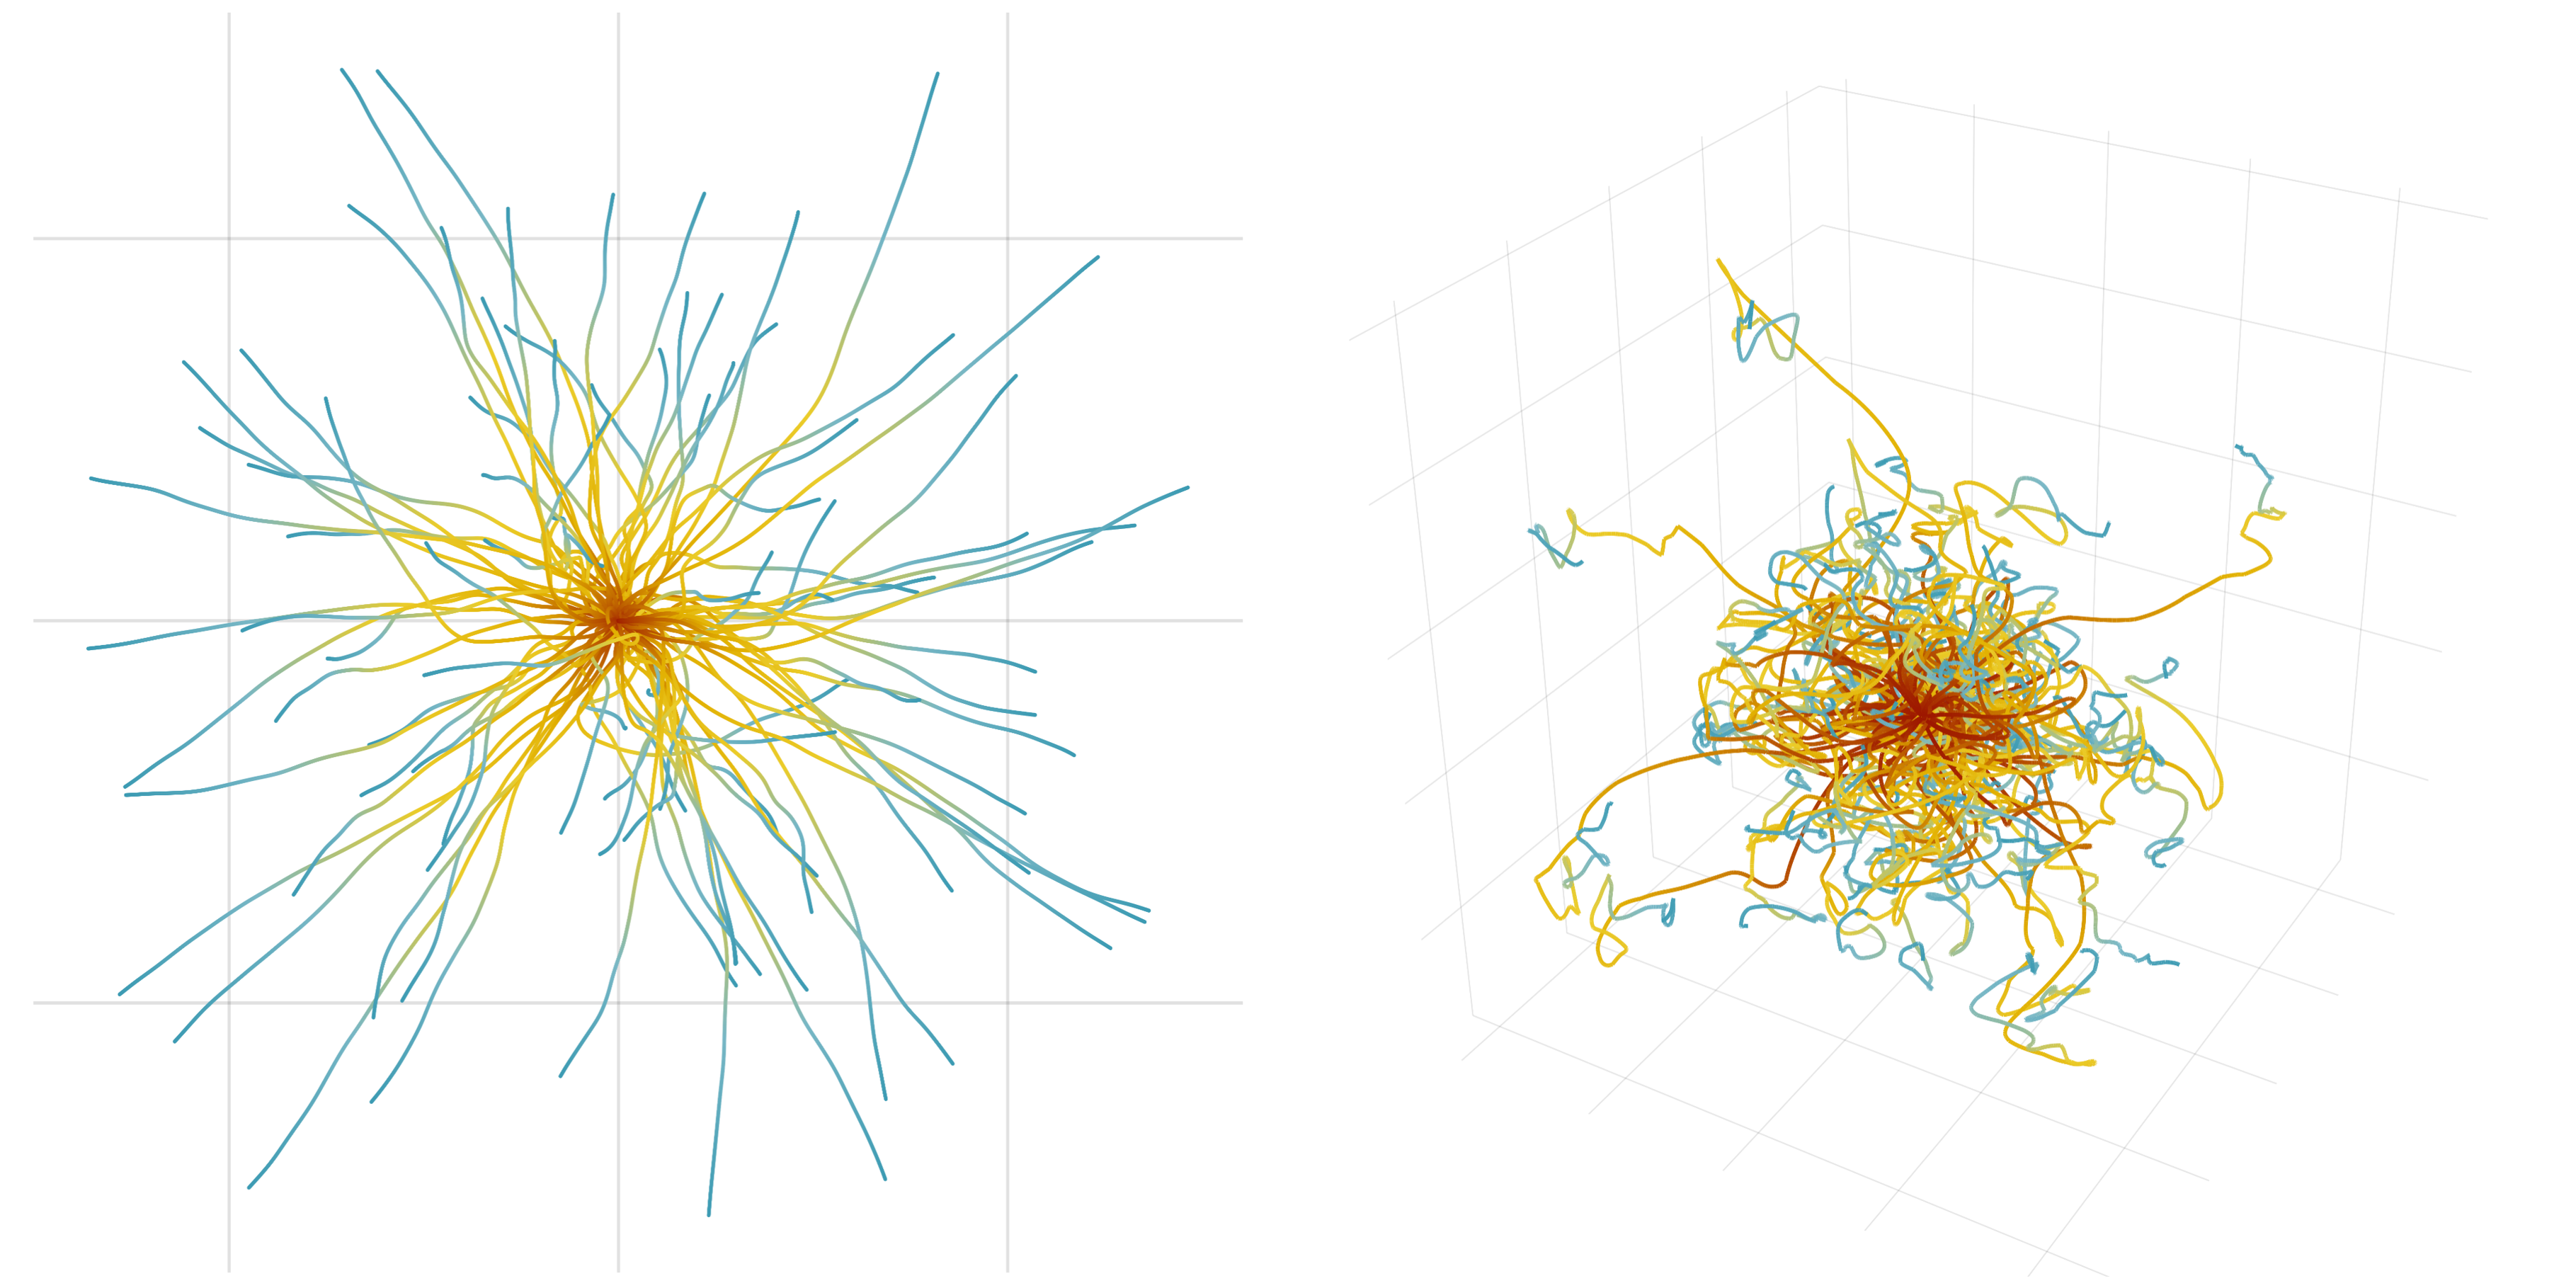
\includegraphics[height=0.7\paperheight]{images/trajectories_cpic.png}} 
    \\[10pt]  
   };
}
\begin{frame}{Outline}
    \begin{center}
        \tableofcontents
    \end{center}
\end{frame}
\setbeamertemplate{background}{}

\setcounter{framenumber}{0}
\setbeamertemplate{footline}[progress bar]
\setbeamercolor{progress bar}{fg=palteal,bg=palteal!40}
\addtobeamertemplate{headline}{}{\vspace{1cm}\hfill\circcounter\hspace*{1cm}}
\addtobeamertemplate{frametitle}{\vspace{-0.8cm}}{}

% %%%%%%%%%%%%%%%%%%%%%%%%%%%%%%%%%%%%%%%%%
% %%%%%%%%%%%%%%%% SECTION %%%%%%%%%%%%%%%%
% %%%%%%%%%%%%%%%%%%%%%%%%%%%%%%%%%%%%%%%%%

% \section{Introduction}

% %%%%%%%%%%%%%%%%%%%%%%%%%%%%%%%%%%%%%%%%%
% %%%%%%%%%%%%%% SUBSECTION %%%%%%%%%%%%%%%
% %%%%%%%%%%%%%%%%%%%%%%%%%%%%%%%%%%%%%%%%%

% \subsection{Stages}

% %%%%%%%%%%%%%%%%%%%%%%%%%%%%%%%%%%%%%%%%%
% %%%%%%%%%%%%%%%%% SLIDE %%%%%%%%%%%%%%%%%
% %%%%%%%%%%%%%%%%%%%%%%%%%%%%%%%%%%%%%%%%%

% \begin{frame}
%     \frametitle{Heavy-ion collisions}
%     \framesubtitle{Stages at weak coupling}
%     \vspace{-15pt}
%     \begin{columns}[onlytextwidth,t]
%         \column{.02\textwidth}
%         \column{.47\textwidth}
%             \begin{center}
%                 \vspace{-5pt}
%                 \begin{tikzpicture}
%                     \node[anchor=south west,inner sep=0] at (0,0) {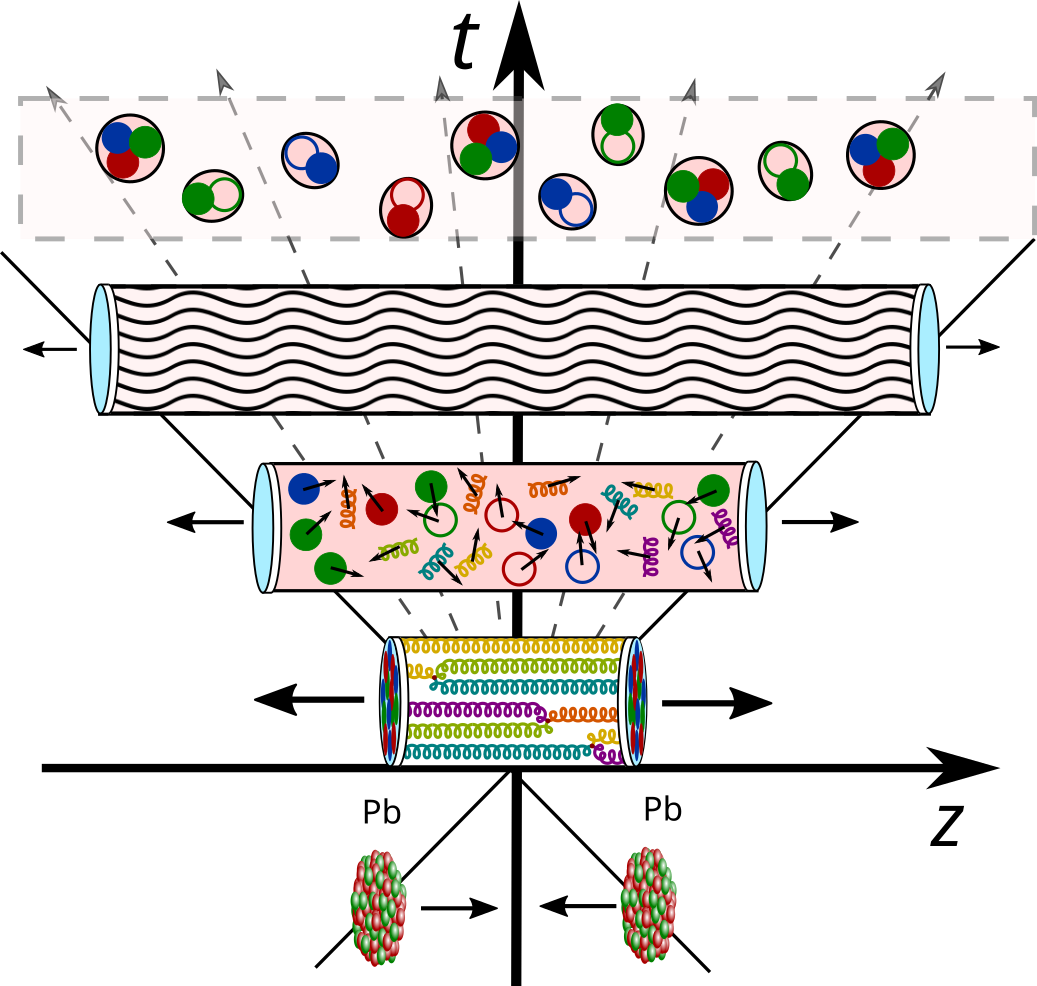
\includegraphics[width=0.95\textwidth]{images/cover_figure_A01.png}};
%                 \end{tikzpicture}
%             \end{center}
%         \column{.02\textwidth}
%         \column{.47\textwidth}
%             \vspace{10pt}
%             \begin{center}
%             \begin{custombox2}{\color{normal}Collision stages}{lightgray}
%                 \small
%                 \begin{varwidth}{0.8\textwidth}
%                 \begin{itemize}\itemsep0em 
%                     \setbeamertemplate{itemize item}{\raisebox{0.2em}{\scalebox{0.7}{${\color{normal}\blacktriangleright}$}}} 
%                     \item {Before collision {\scriptsize $\tau\leq 0\,\mathrm{fm/c}$}}\\[1pt]
%                         {\color{lightgray}\scriptsize Gluon field of high-energy nucleus}
%                     \setbeamertemplate{itemize item}{\raisebox{0.2em}{\scalebox{0.7}{${\color{palviolet}\blacktriangleright}$}}} \item {{\bfseries\color{palviolet} Initial stage} {\scriptsize $\tau\lesssim
%                     0.3\,\mathrm{fm/c}$}}\\[1pt]
%                         {\color{lightgray}\scriptsize {\bfseries\color{palviolet}Glasma} strong classical gluon fields}
%                     \setbeamertemplate{itemize item}{\raisebox{0.2em}{\scalebox{0.7}{${\color{normal}\blacktriangleright}$}}} \item Thermalization {\scriptsize$\tau\lesssim
%                     1\,\mathrm{fm/c}$}\\[1pt] 
%                         {\color{lightgray}\scriptsize Effective kinetic theory} 
%                         % \\ {\color{lightgray}\scriptsize Quasiparticle distribution function}
%                     \item Equilibration {\scriptsize $\tau\lesssim 10\,\mathrm{fm/c}$}\\[1pt]
%                     {\color{lightgray}\scriptsize Relativistic hydrodynamics} 
%                     % \\ {\color{lightgray}\scriptsize Energy-momentum tensor}
%                     \item Final stages {\scriptsize $\tau\geq 10\,\mathrm{fm/c}$}\\[1pt]
%                     {\color{lightgray}\scriptsize Particlization, hadronization}
%                 \end{itemize}
%                 \end{varwidth}
%             \end{custombox2}
%             \end{center}
%         \column{.02\textwidth}
%     \end{columns}
%     \blfootnote{\scriptsize Berges, Heller, Mazeliauskas, Venugopalan \href{https://arxiv.org/abs/2005.12299}{{\color{palgold}\texttt{[2005.12299]$^\text{\tiny\faExternalLink}$}}}, Schlichting, Teaney \href{https://arxiv.org/abs/1908.02113}{{\color{palgold}\texttt{[1908.02113]$^\text{\tiny\faExternalLink}$}}}}
% \end{frame}

% \subsection{Initial stage}

% %%%%%%%%%%%%%%%%%%%%%%%%%%%%%%%%%%%%%%%%%
% %%%%%%%%%%%%%%%%% SLIDE %%%%%%%%%%%%%%%%%
% %%%%%%%%%%%%%%%%%%%%%%%%%%%%%%%%%%%%%%%%%

% \begin{frame}[noframenumbering]
%     \frametitle{Initial stage of collision}
%     % \framesubtitle{Stages at weak coupling}
%     \vspace{-10pt}
%     \begin{columns}[onlytextwidth,t]
%         \column{.02\textwidth}
%         \column{.47\textwidth}
%             \begin{center}
%                 \vspace{-5pt}
%                 \begin{tikzpicture}
%                     \node[anchor=south west,inner sep=0] at (0,0) {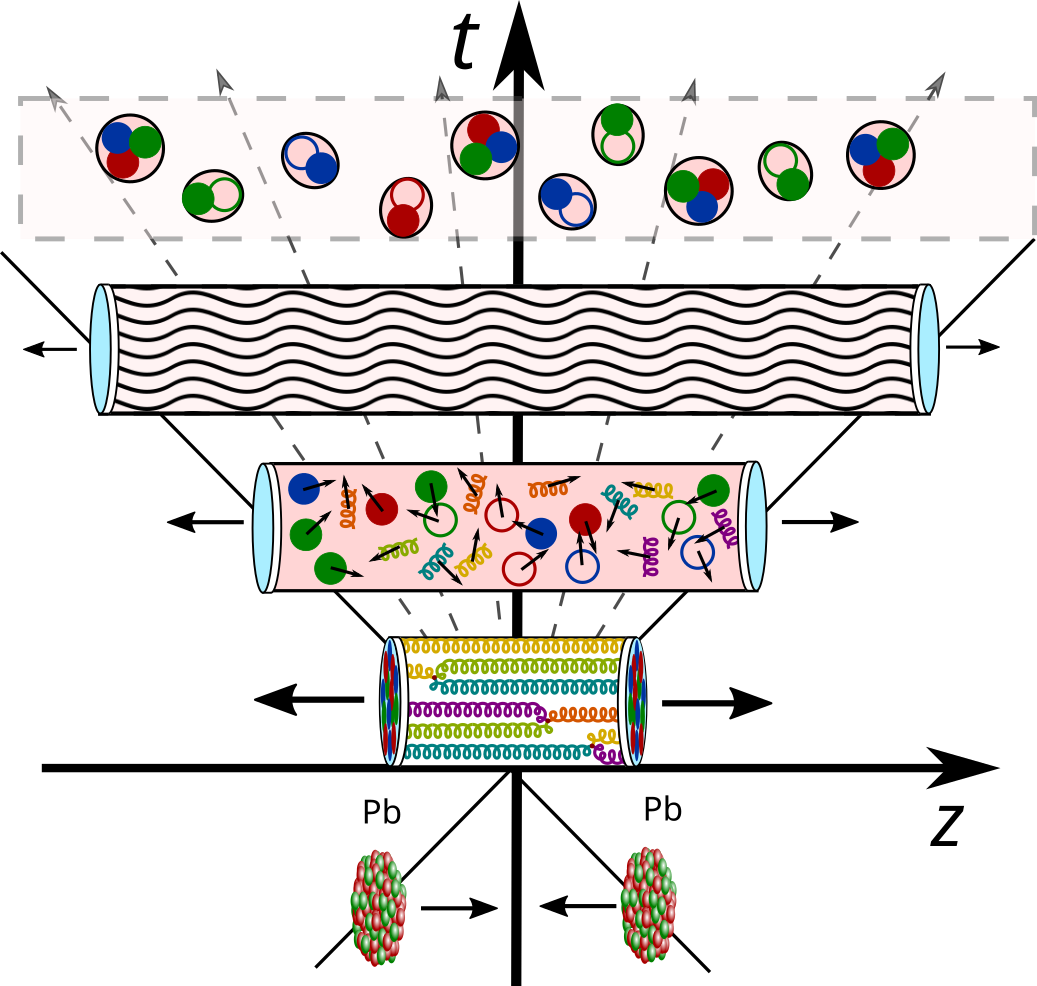
\includegraphics[width=0.95\textwidth]{images/cover_figure_A01.png}};
%                     \draw<1>[white, fill=white, fill opacity=0.9] (0.0,2.45) rectangle (6.8,6.5);
%                     \draw<1>[palviolet,thick,fill=palviolet,fill opacity=0.1,rounded corners=3pt] (0.1,-0.1) rectangle (6.7,2.45);
%                 \end{tikzpicture}
%             \end{center}
%         \column{.02\textwidth}
%         \column{.47\textwidth}
%             \vspace{7pt}
%             \begin{center}
%             \begin{custombox2}{Glasma initial stage}{palviolet}
%                 \small
%                 \begin{varwidth}{0.76\textwidth}
%                 \begin{itemize}\itemsep0em 
%                     \setbeamertemplate{itemize item}{\raisebox{0.2em}{\scalebox{0.7}{${\color{palviolet}\blacktriangleright}$}}} 
%                     \item {Color glass condensate}\\[1pt]
%                         {\color{lightgray}\scriptsize QCD in the high-energy limit}
%                     \item Weakly coupled $\alpha_s\ll 1$
%                     \item {\bfseries Classical gluon fields}\\[1pt]
%                         {\color{lightgray}\scriptsize Occupation number $\sim 1/\alpha_s\gg 1$}
%                     \item {\bfseries Non-perturbative} regime
%                     % \item {\bfseries Lattice gauge theory}\\[1pt]
%                         % {\color{lightgray}\scriptsize Numerical solution}
%                     \item {\bfseries Out-of-equilibrium} medium
                    
%                 \end{itemize}
%                 \end{varwidth}
%             \end{custombox2}

%             \begin{custombox2}{Hard probes}{palteal}
%                 \small
%                 \begin{varwidth}{0.68\textwidth}
%                 \begin{itemize}\itemsep0em 
%                     \setbeamertemplate{itemize item}{\raisebox{0.2em}{\scalebox{0.7}{${\color{palteal}\blacktriangleright}$}}} 
%                     \item Jets and heavy quarks\\[1pt]
%                     {\color{lightgray}\scriptsize Produced in the initial stage}
%                     {\color{lightgray}\scriptsize Kinematics large $E$/large $m$}
%                 \end{itemize}
%                 \end{varwidth}
%             \end{custombox2}
%             \end{center}
%         \column{.02\textwidth}
%     \end{columns}
%     \blfootnote{\scriptsize Lappi \href{https://arxiv.org/abs/hep-ph/0606207}{{\color{palviolet}\texttt{[hep-ph/0606207]}$^\text{\tiny\faExternalLink}$}}, Gelis \href{https://arxiv.org/abs/1211.3327}{{\color{palviolet}\texttt{[1211.3327]}$^\text{\tiny\faExternalLink}$}}}
% \end{frame}


% %%%%%%%%%%%%%%%%%%%%%%%%%%%%%%%%%%%%%%%%%
% %%%%%%%%%%%%%% SUBSECTION %%%%%%%%%%%%%%%
% %%%%%%%%%%%%%%%%%%%%%%%%%%%%%%%%%%%%%%%%%

% \subsection{Hard probes}

% %%%%%%%%%%%%%%%%%%%%%%%%%%%%%%%%%%%%%%%%%
% %%%%%%%%%%%%%%%%% SLIDE %%%%%%%%%%%%%%%%%
% %%%%%%%%%%%%%%%%%%%%%%%%%%%%%%%%%%%%%%%%%

% \setbeamertemplate{background}{
% \tikz[overlay,remember picture] \node[at=(current page.center), align=center] {\\[10pt]
% {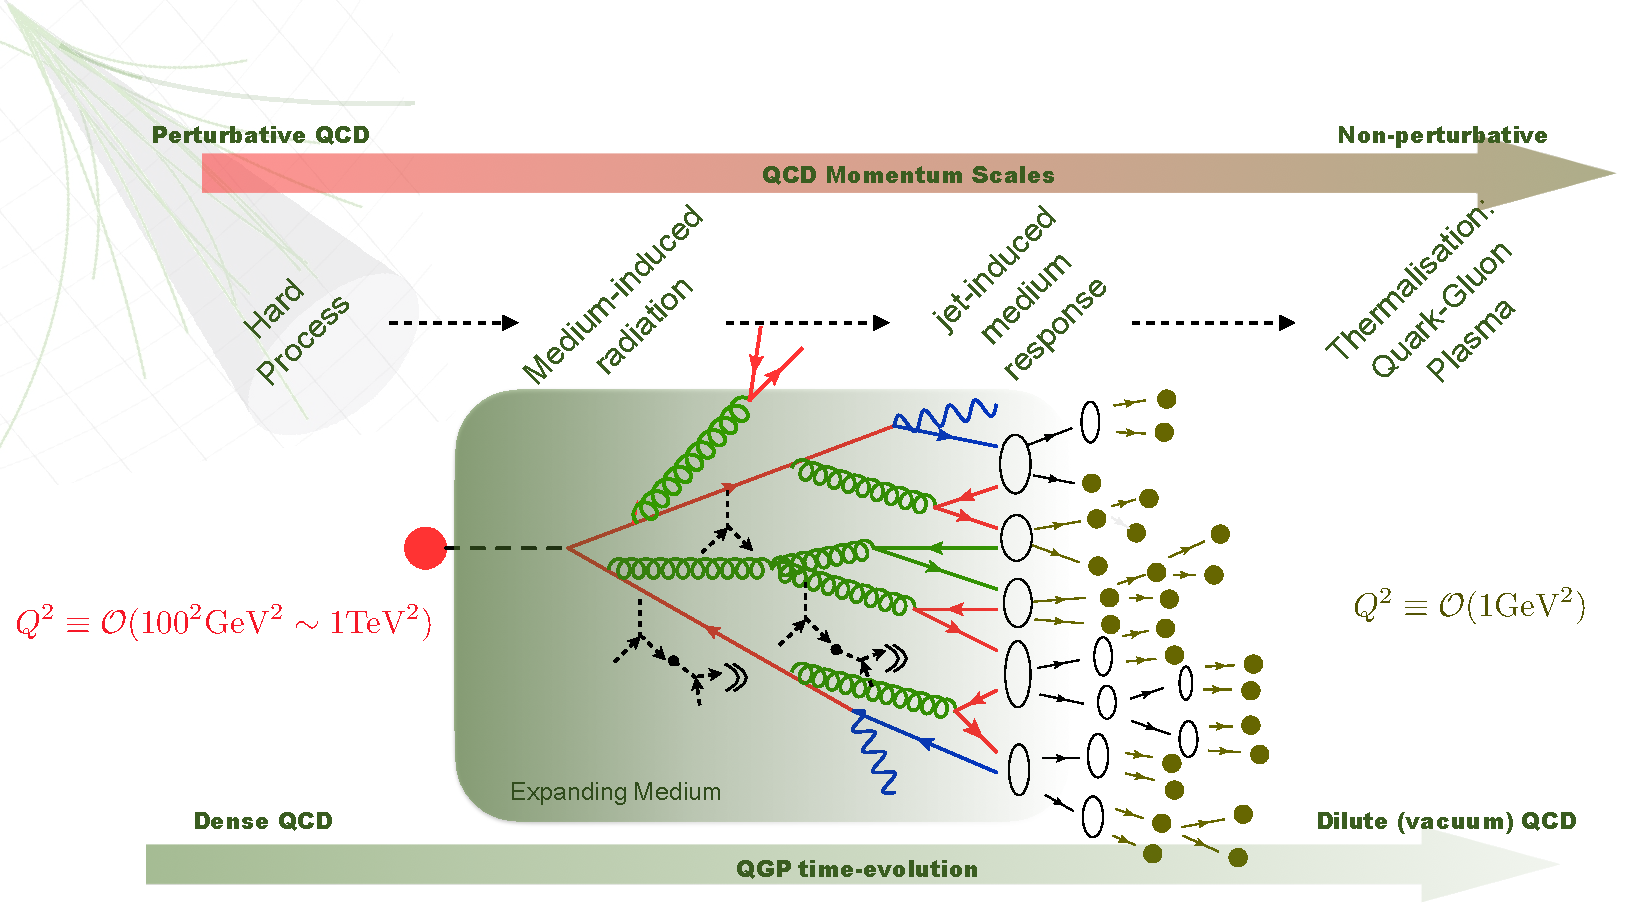
\includegraphics[height=0.8\paperheight]{images/Holmganga_jets_Liliana-scales.pdf}}};
% }
% \begin{frame}
%     \frametitle{Jets as probes}
%     \framesubtitle{Stages and scales of interest}
%     \blfootnote{\scriptsize Apolinario - \textit{Jetography via the Quark-Gluon Plasma} \href{https://indico.cern.ch/event/1385550/}{{\color{red}\texttt{[CERN 24]$^\text{\tiny\faExternalLink}$}}}}
% \end{frame}
% \setbeamertemplate{background}{}

% %%%%%%%%%%%%%%%%%%%%%%%%%%%%%%%%%%%%%%%%%
% %%%%%%%%%%%%%%%%% SLIDE %%%%%%%%%%%%%%%%%
% %%%%%%%%%%%%%%%%%%%%%%%%%%%%%%%%%%%%%%%%%

% \setbeamertemplate{background}{
% \tikz[overlay,remember picture] \node[at=(current page.center), align=center] {\\[-5pt]
% {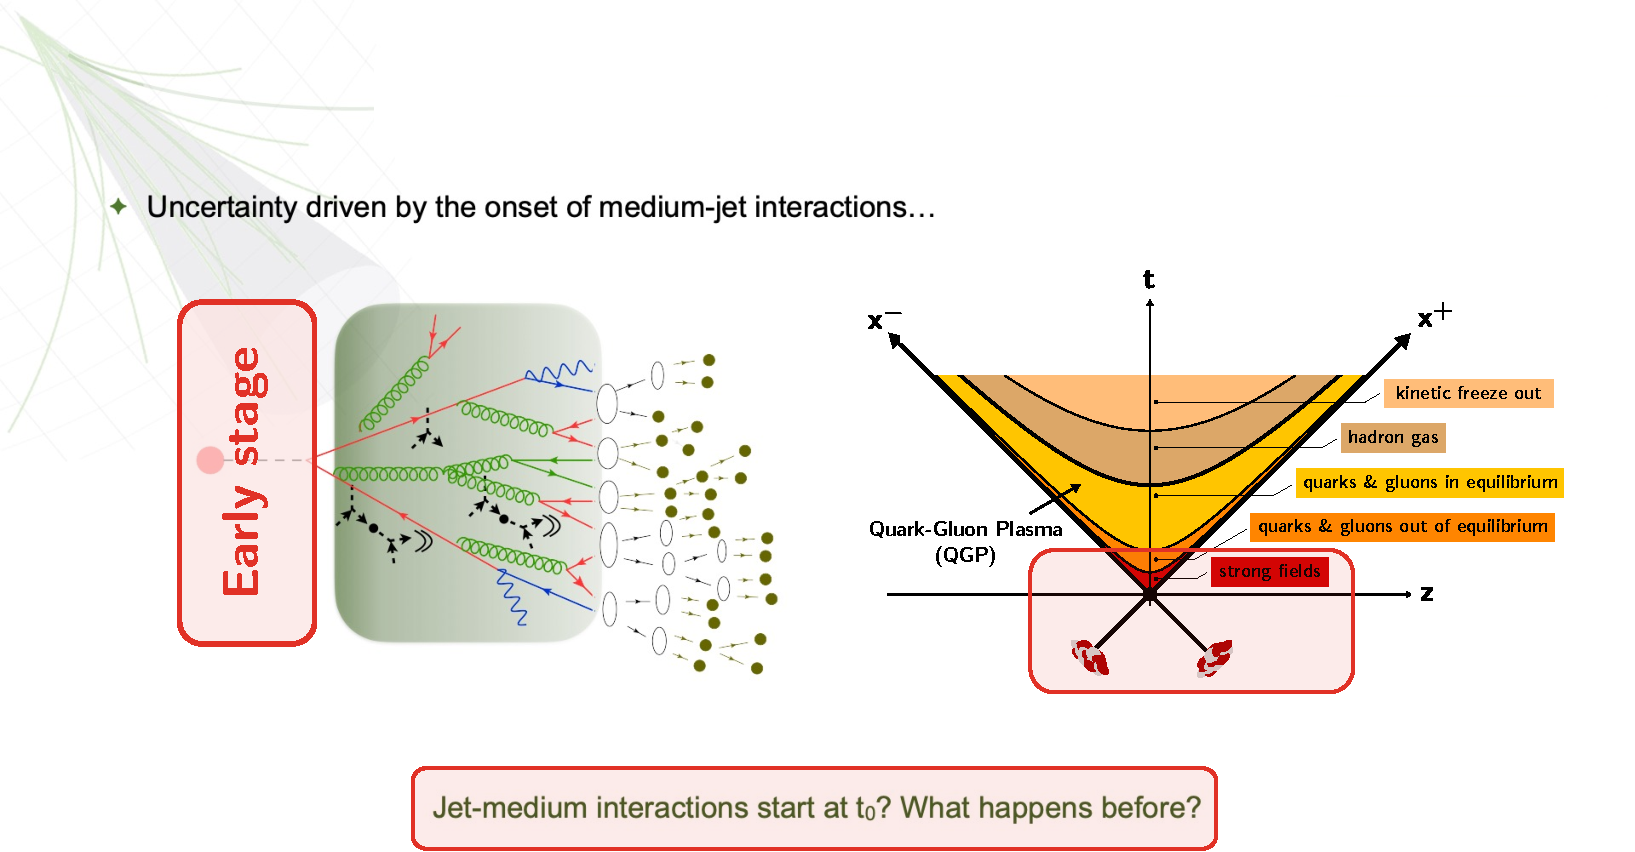
\includegraphics[height=0.8\paperheight]{images/LApolinario_HP23-modelling-early.pdf}}};
% }
% \begin{frame}[noframenumbering]
%     \frametitle{Jets as probes of the {\color{red}early stage}}
%     % \framesubtitle{Stages and scales of interest}
%     \blfootnote{\scriptsize Apolinario - \textit{Monte Carlo modeling of jets} \href{https://indico.uni-muenster.de/event/1409/contributions/2412/}{{\color{red}\texttt{[Plenary Hard Probes 23]$^\text{\tiny\faExternalLink}$}}}, adapted}
% \end{frame}
% \setbeamertemplate{background}{}

% %%%%%%%%%%%%%%%%%%%%%%%%%%%%%%%%%%%%%%%%%
% %%%%%%%%%%%%%%%%% SLIDE %%%%%%%%%%%%%%%%%
% %%%%%%%%%%%%%%%%%%%%%%%%%%%%%%%%%%%%%%%%%

% \begin{frame}
%     \frametitle{Heavy quarks as probes}
%     \framesubtitle{Approaches and kinematic regimes}

%     \begin{columns}[onlytextwidth,t]
%         \column{.02\textwidth}
%         \column{.57\textwidth}
%             \vspace{-20pt}
%             \begin{center}
%                 \begin{tikzpicture}
%                     \node[anchor=south west,inner sep=0] at (0,0) {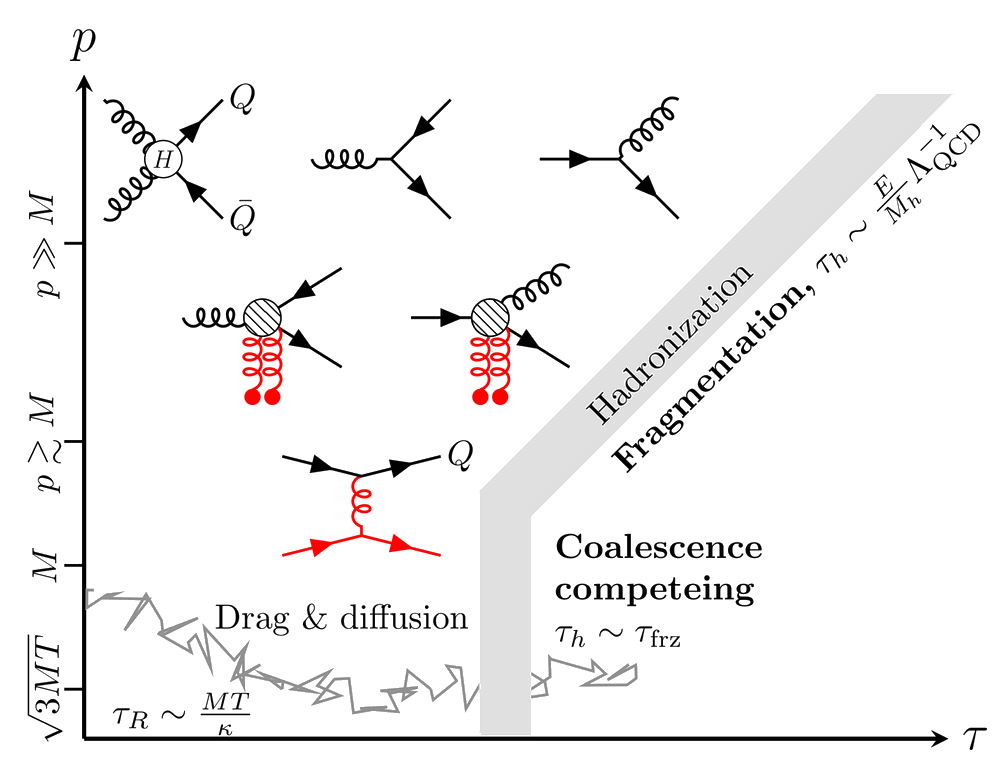
\includegraphics[width=0.95\textwidth]{images/HP24-Weiyao-Ke-HF-Theory-2-crop-white.png}};
%                 \end{tikzpicture}
%             \end{center}
%         \column{.02\textwidth}
%         \column{.37\textwidth}
%         \vspace{10pt}
%         \begin{center}
%             \begin{custombox2}{\color{normal}Approaches}{lightgray}
%                 \small
%                 \begin{varwidth}{0.85\textwidth}
%                 \begin{itemize}\itemsep0em 
%                     \setbeamertemplate{itemize item}{\raisebox{0.2em}{\scalebox{0.7}{${\color{normal}\blacktriangleright}$}}} 
%                     \item pQCD production\\[1pt]
%                         {\color{lightgray}\scriptsize FONLL and GM-VFNS at NLO+NLL accuracy}
%                     \item Transport models\\[1pt]
%                         {\color{lightgray}\scriptsize Boltzmann, Langevin, Fokker-Planck equations}
%                     \item Hadronization\\[1pt]
%                         {\color{lightgray}\scriptsize Fragmentation + coalescence}  
%                 \end{itemize}
%                 \end{varwidth}
%             \end{custombox2}
%             \end{center}
%         \column{.02\textwidth}
%     \end{columns}

%     \vspace{-5pt}    
%     \blfootnote{\scriptsize Ke - \textit{Open Heavy Flavor: Theory} \href{https://indico.cern.ch/event/1339555/contributions/6038190/}{{\color{red}\texttt{[Plenary Hard Probes 24]$^\text{\tiny\faExternalLink}$}}}}
% \end{frame}

% %%%%%%%%%%%%%%%%%%%%%%%%%%%%%%%%%%%%%%%%%
% %%%%%%%%%%%%%%%%% SLIDE %%%%%%%%%%%%%%%%%
% %%%%%%%%%%%%%%%%%%%%%%%%%%%%%%%%%%%%%%%%%

% \begin{frame}[noframenumbering]
%     \frametitle{Heavy quarks as probes of the {\color{red}early stage}}
%     % \framesubtitle{Recent focus on the early stage}

%     \begin{center}
%         \begin{tikzpicture}
%             \node[anchor=south west,inner sep=0] at (0,0) {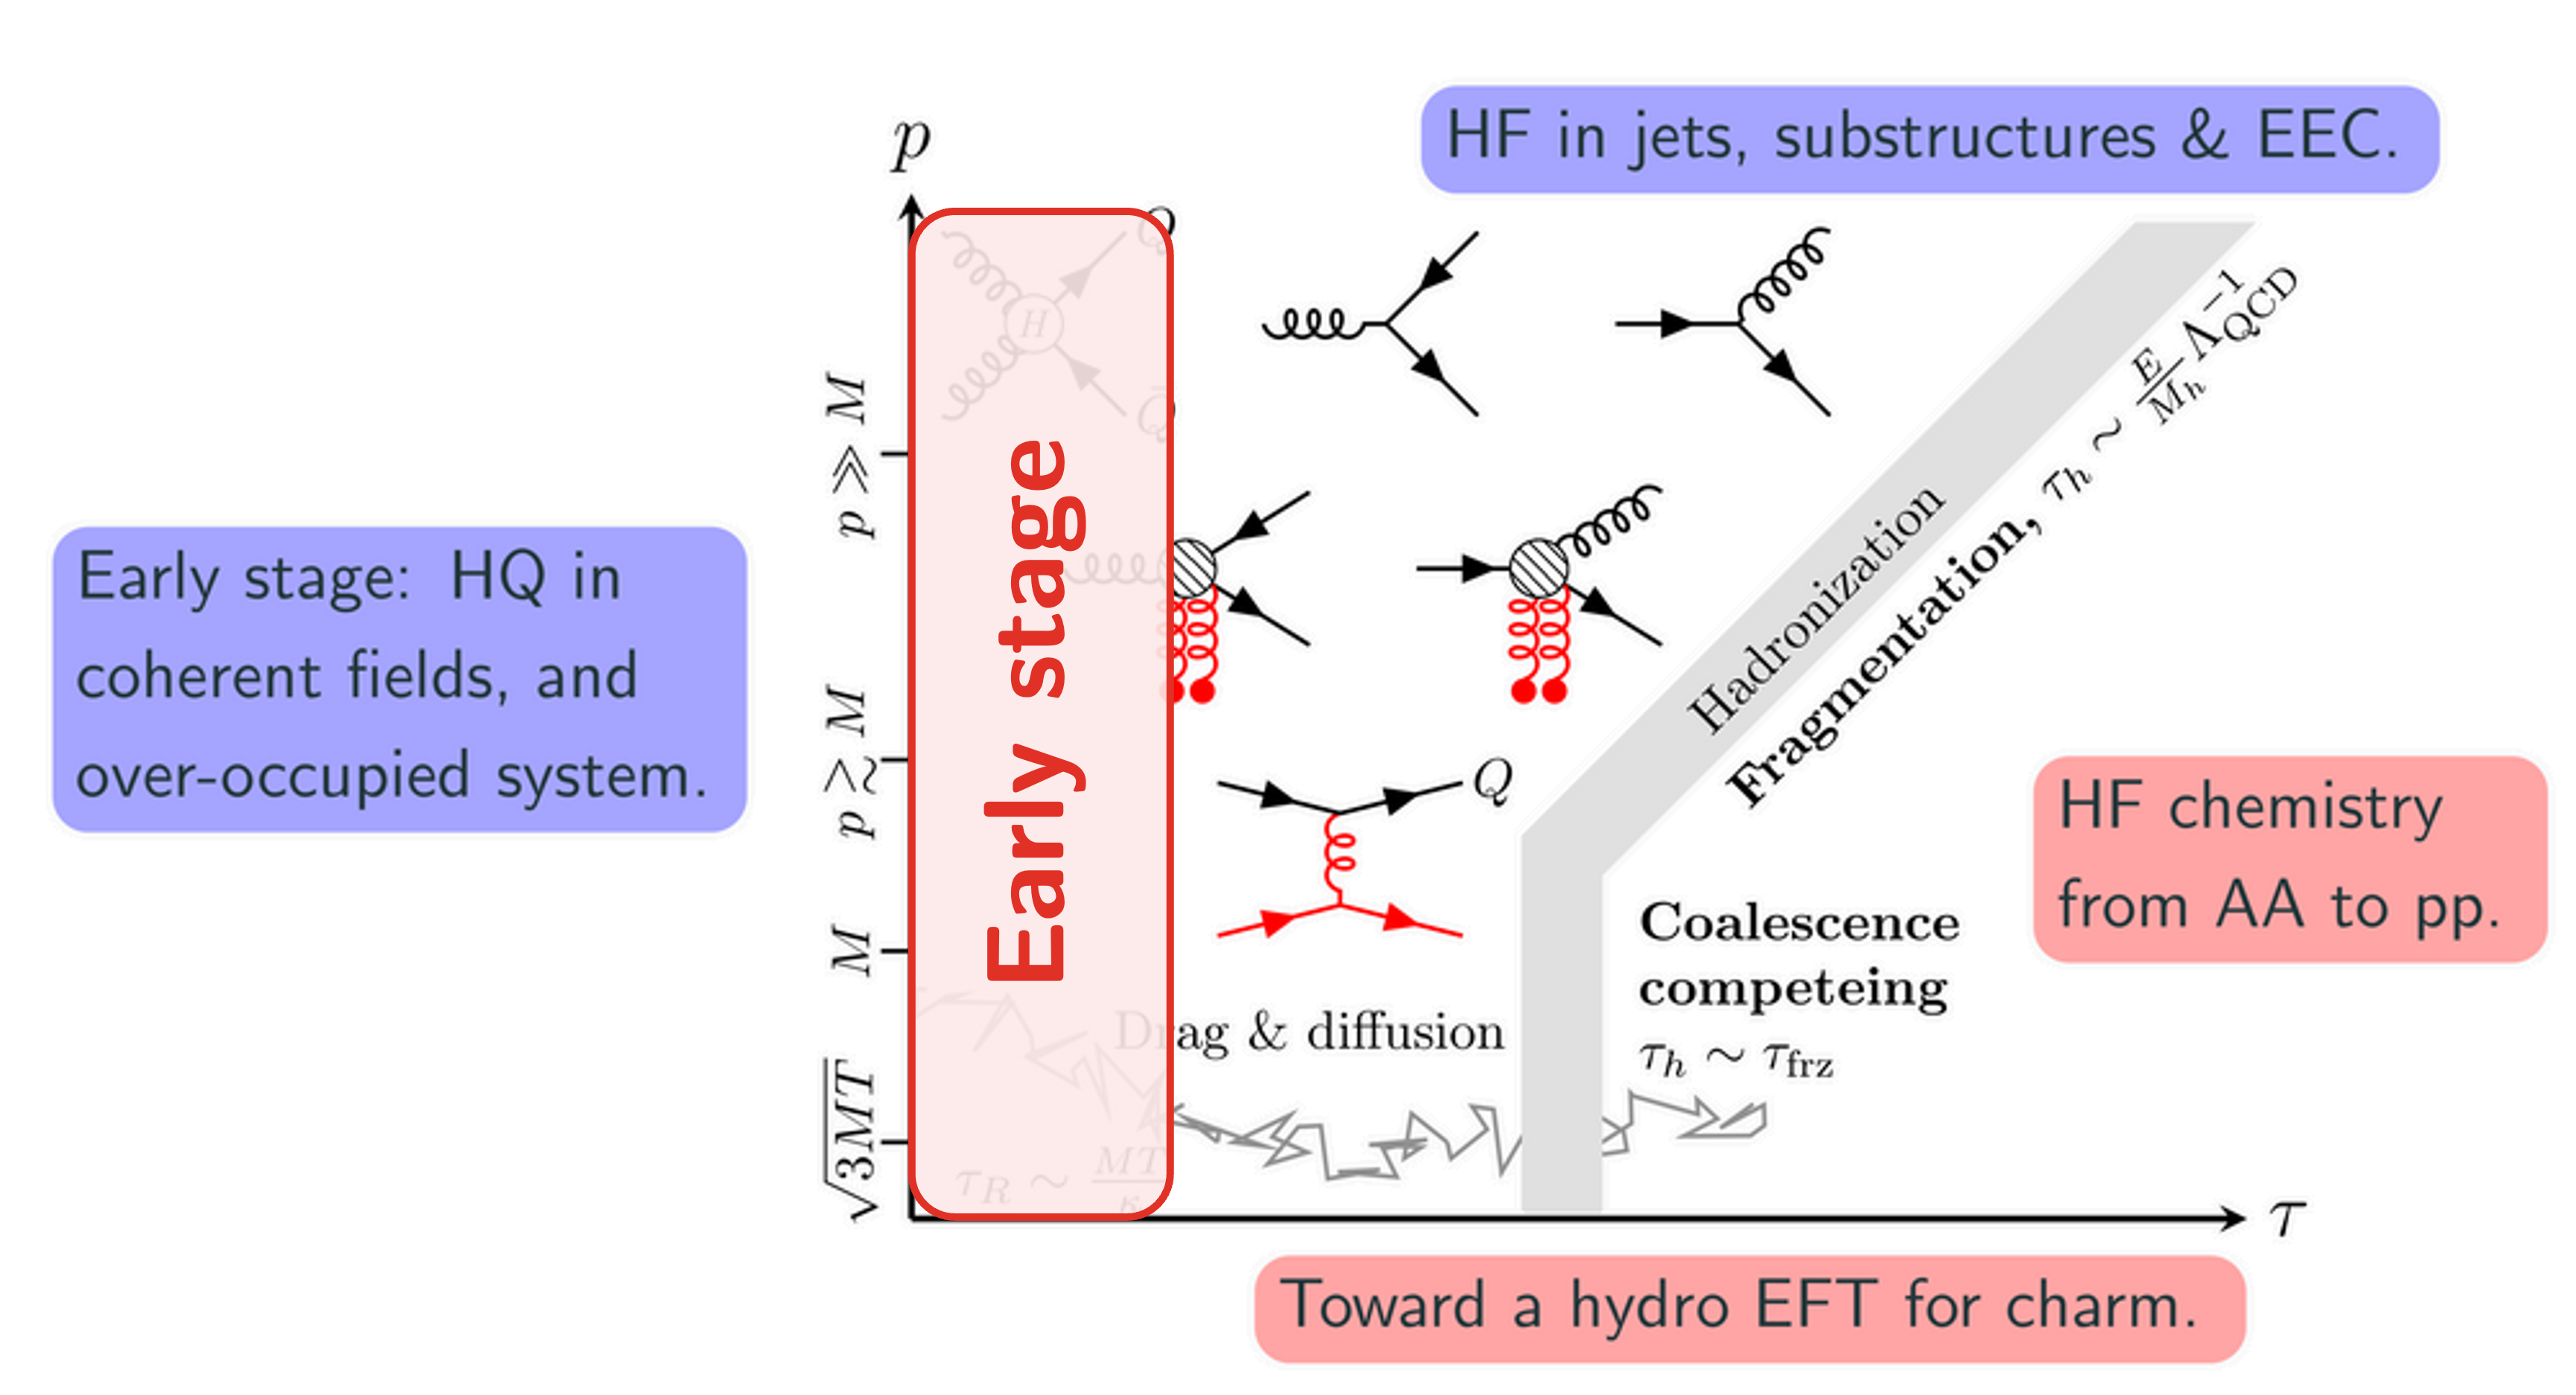
\includegraphics[width=0.8\textwidth]{images/HP24-Weiyao-Ke-HF-Theory-28-crop-white-edit.png}};
%             % \draw<1>[palgold,thick,fill=palgold,fill opacity=0.1,rounded corners=3pt] (0.0,4) rectangle (\textheight-0.5cm,4.0) node[opacity=1.0, pos=0, anchor=center, xshift=0.0\linewidth,text width=2cm,align=center]{{\Large\color{palgold}\bfseries This talk}};
%             % \draw<1>[white, fill=white, fill opacity=0.9] (4.3,0.85) rectangle (5.4,5.5);
%             % \draw<1>[red,thick,fill=red,fill opacity=0.1,rounded corners=3pt] (4.3,0.85) rectangle (5.4,5.5) node[opacity=1.0, pos=0.5, rotate=90, anchor=center, xshift=0.0 ,text width=6.2cm,align=center] {{\Large\color{red} Early stage}};
%         \end{tikzpicture}
%     \end{center}
%     \vspace{-10pt}    
%     \blfootnote{\scriptsize Ke - \textit{Open Heavy Flavor: Theory} \href{https://indico.cern.ch/event/1339555/contributions/6038190/}{{\color{red}\texttt{[Plenary Hard Probes 24]$^\text{\tiny\faExternalLink}$}}}, adapted}
% \end{frame}



%%%%%%%%%%%%%%%%%%%%%%%%%%%%%%%%%%%%%%%%%
%%%%%%%%%%%%%%%% SECTION %%%%%%%%%%%%%%%%
%%%%%%%%%%%%%%%%%%%%%%%%%%%%%%%%%%%%%%%%%

\section{Glasma fields}

%%%%%%%%%%%%%%%%%%%%%%%%%%%%%%%%%%%%%%%%%
%%%%%%%%%%%%%%%%% SLIDE %%%%%%%%%%%%%%%%%
%%%%%%%%%%%%%%%%%%%%%%%%%%%%%%%%%%%%%%%%%

\setbeamertemplate{background}{
\tikz[overlay,remember picture] \node[opacity=0.1, at=(current page.center), align=center] {\\[10pt]
{\transparent{0.2}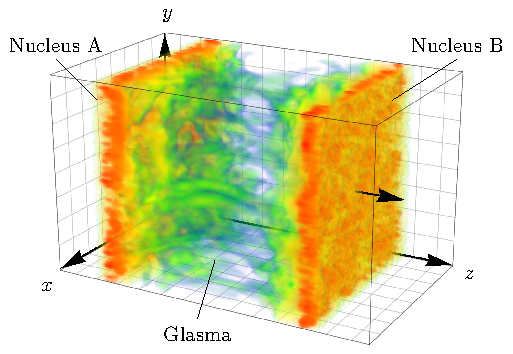
\includegraphics[height=0.8\paperheight]{images/fig1_overview.pdf}}};
}
\begin{frame}[plain,noframenumbering]{}
    \begin{center}
        \vspace{1cm}
        {\large\color{normal}Initial stage of pre-equilibrium}\\[0.3cm]
        {\huge\color{destacado}The glasma}
    \end{center}
\end{frame}
\setbeamertemplate{background}{}

%%%%%%%%%%%%%%%%%%%%%%%%%%%%%%%%%%%%%%%%%
%%%%%%%%%%%%%%%%% SLIDE %%%%%%%%%%%%%%%%%
%%%%%%%%%%%%%%%%%%%%%%%%%%%%%%%%%%%%%%%%%

\setbeamertemplate{background}{
\tikz[overlay,remember picture] \node[at=(current page.center), align=center] {\\[10pt]
{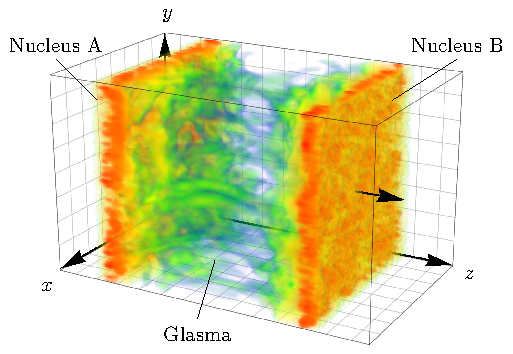
\includegraphics[height=0.7\paperheight]{images/fig1_overview.pdf}}};
}
\begin{frame}[plain,noframenumbering]
    \frametitle{\\ Glasma color fields}
    \blfootnote{\scriptsize Ipp, Müller  \href{https://arxiv.org/abs/1703.00017}{{\color{palgold}\texttt{[1703.00017]}$^\text{\tiny\faExternalLink}$}}}
\end{frame}
\setbeamertemplate{background}{}

% %%%%%%%%%%%%%%%%%%%%%%%%%%%%%%%%%%%%%%%%%
% %%%%%%%%%%%%%% SUBSECTION %%%%%%%%%%%%%%%
% %%%%%%%%%%%%%%%%%%%%%%%%%%%%%%%%%%%%%%%%%

% \subsection{CGC}

% %%%%%%%%%%%%%%%%%%%%%%%%%%%%%%%%%%%%%%%%%
% %%%%%%%%%%%%%%%%% SLIDE %%%%%%%%%%%%%%%%%
% %%%%%%%%%%%%%%%%%%%%%%%%%%%%%%%%%%%%%%%%%

% \setbeamertemplate{itemize item}{\raisebox{0.2em}{\scalebox{0.7}{${\color{normal}\blacktriangleright}$}}} 

% \begin{frame}
%     \frametitle{Color glass condensate}
%     \framesubtitle{QCD at high energy and glasma fields}
%     \vspace{-15pt}
%     \begin{columns}[onlytextwidth,t]
%        \column{.033\textwidth}
%        \column{.35\textwidth}

%             \begin{center}
%                 \footnotesize\color{lightgray}A high-energy nucleus contains \\ large numbers of {\bfseries\color{palviolet}soft gluons}
%             \end{center}
%             % \begin{itemize}\itemsep0em 
%             %     \footnotesize\color{lightgray}
%             %     \setbeamertemplate{itemize item}{\raisebox{0.2em}{\scalebox{0.6}{${\color{lightgray}\blacktriangleright}$}}}
%             %     \item A high-energy nucleus contains mostly {\bfseries\color{palviolet}soft gluons}
%             % \end{itemize}

%             \vspace{0pt}
%             \hspace{10pt}
%             \begin{tikzpicture}[]
%                 \node[anchor=south west,inner sep=0] at (0,0) {\includegraphics[width=0.9\textwidth]{images/CFNS_talk_Salazar-3_crop_edit_final_v2.png}};
%                 \draw<1>[palviolet,line width=1pt,fill=palviolet,fill opacity=0.1,rounded corners=3pt] (2.2, 0) rectangle (4.8, 4.9);
%             \end{tikzpicture}
%         \column{.06\textwidth}
%         \column{.55\textwidth}

%             \vspace{0pt}
           
%             \begin{custombox2}{Color glass condensate}{lightgray}
%                 \small
%                 \begin{varwidth}{0.92\textwidth}
%                 \begin{itemize}\itemsep0em 
%                     \setbeamertemplate{itemize item}{\raisebox{0.2em}{\scalebox{0.7}{${\color{lightgray}\blacktriangleright}$}}} 
%                     \item 
%                     Soft partons $\leftrightarrow$ {\color{palviolet}\bfseries gauge fields $\boldsymbol{A^\mu}$} generated \\ by the hard partons $\leftrightarrow$ {\color{palteal}\bfseries color current $\boldsymbol{J^\mu}$}
%                 \end{itemize}
%                 \end{varwidth}
%             \end{custombox2}

%             % \begin{itemize}\itemsep0em 
%             %     \footnotesize\color{lightgray}
%             %     \setbeamertemplate{itemize item}{\raisebox{0.2em}{\scalebox{0.6}{${\color{lightgray}\blacktriangleright}$}}}
%             %     \item Classical {\color{palviolet}gluon fields} $\rightarrow$ produced\\ by color {\color{pallightblue}nucleus current}
%             % \end{itemize}
%             \begin{itemize}\itemsep0em 
%                 \item Classical Yang-Mills equations
%             \end{itemize}
%             \vspace{20pt}
%             \renewcommand{\eqnhighlightheight}{\vphantom{\mathcal{D}_\mu}\mathstrut}\begin{equation*}
%                 \hspace{-40pt}\eqnmark[normal]{dmu}{\mathscr{D}_\mu}\hspace{-3pt}\eqnmark[normal]{fmunu}{F^{\mu\nu}}\hspace{-3pt}={\color{palteal}\boldsymbol{J^\nu}}
%                 % {\color{lightgray}\rightarrow\,\text{input from CGC}} 
%                 \end{equation*}
%                 \annotate[yshift=+0.5em]{above, left}{dmu}{\scriptsize $\partial_\mu-\mathrm{i}g{\color{palviolet}\boldsymbol{A_\mu}}$}
%                 \annotate[yshift=-0.1em]{below}{fmunu}{\scriptsize $\partial_\mu{\color{palviolet}\boldsymbol{A_\nu}}-\partial_\nu{\color{palviolet}\boldsymbol{A_\mu}}-\mathrm{i}g[{\color{palviolet}\boldsymbol{A_\mu}},{\color{palviolet}\boldsymbol{A_\nu}}]$}
%             \vspace{5pt}
%             {\footnotesize
%             \begin{itemize}\itemsep0em 
%                 % \setbeamertemplate{itemize item}{\raisebox{0.2em}{\scalebox{0.6}{${\color{lightgray}\blacktriangleright}$}}} 
%                 \item \textit{Before collision:} CGC fields\\[1pt] 
%                 {\color{lightgray} Analytical gluon field of a single nucleus}
%                 \item \textit{After collision:} {\color{palgold}\bfseries glasma fields}\\[1pt] 
%                 {\color{lightgray} Numerical gluon field of two colliding nuclei}
%             \end{itemize}}
%         \column{.033\textwidth}
%     \end{columns}
%     \blfootnote{\scriptsize Gelis, Iancu, Jalilian-Marian, Venugopalan \href{https://arxiv.org/abs/1002.0333}{{\color{palviolet}\texttt{[1002.0333]}$^\text{\tiny\faExternalLink}$}}, Lappi \href{https://arxiv.org/abs/hep-ph/0602189}{{\color{palgold}\texttt{[hep-ph/0602189]}$^\text{\tiny\faExternalLink}$}}}
% \end{frame}

% %%%%%%%%%%%%%%%%%%%%%%%%%%%%%%%%%%%%%%%%%
% %%%%%%%%%%%%%%%%% SLIDE %%%%%%%%%%%%%%%%%
% %%%%%%%%%%%%%%%%%%%%%%%%%%%%%%%%%%%%%%%%%

% \begin{frame}
%     \frametitle{CGC fields before collision}
%     \framesubtitle{McLerran-Venugopalan model for AA collisions}
%     \vspace{-10pt}
%     \begin{columns}[onlytextwidth,t]
%         \column{.033\textwidth}
%         \column{.4\textwidth}

%         \begin{center}\itemsep0em 
%             \footnotesize\color{lightgray} Color charge distribution for a nucleus\\ at high energy in a {\bfseries \color{palviolet}thin color sheet}
%         \end{center}

%         \begin{figure}
%             \centering
%             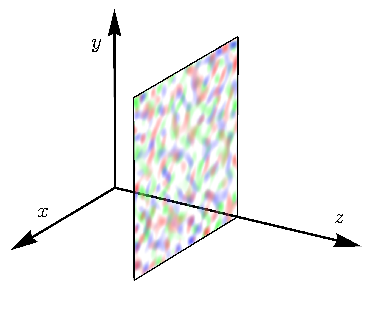
\includegraphics[width=0.9\textwidth]{images/sheets1.pdf}
%         \end{figure}
%        \column{.033\textwidth}
%        \column{.5\textwidth}
%        \vspace{-5pt}
%         \begin{custombox2}{MV model}{lightgray}
%             \small
%             \begin{varwidth}{0.96\textwidth}
%             \begin{itemize}\itemsep0em 
%                 \setbeamertemplate{itemize item}{\raisebox{0.2em}{\scalebox{0.7}{${\color{palteal}\blacktriangleright}$}}} 
%                 \item {\color{palteal}\bfseries Color current} of nucleus $\rightarrow$ generated by \\{\color{palgold}\bfseries color charge} $\color{palgold}\boldsymbol{\rho}$ $\leftrightarrow$ stochastic variable
%             \end{itemize}
%             \end{varwidth}
%         \end{custombox2}

%         % \begin{itemize}\itemsep0em 
%         %     \footnotesize\color{lightgray}
%         %     \setbeamertemplate{itemize item}{\raisebox{0.2em}{\scalebox{0.6}{${\color{lightgray}\blacktriangleright}$}}}
%         %     \item {\color{palteal}Color current} of nucleus $\rightarrow$ generated\\ by {\color{palgold} color charge} density
%         % \end{itemize}
%         \begin{itemize}\itemsep0em 
%             \setbeamertemplate{itemize item}{\raisebox{0.2em}{\scalebox{0.7}{${\color{palgold}\blacktriangleright}$}}}
%             \item {\bfseries\color{palgold} MV model} for color charges ${\color{palgold}\boldsymbol{\rho}}$
%         \end{itemize}
%         \vspace{5pt}
%         \renewcommand{\eqnhighlightheight}{\vphantom{\mathcal{D}_\mu}\mathstrut}\begin{equation*}
%             \big\langle{\color{palgold}\boldsymbol{\rho}}(\vec{x}_\perp){\color{palgold}\boldsymbol{\rho}}(\vec{y}_\perp)\big\rangle\propto\hspace{-3pt}\eqnmark[normal]{g2mu}{{\color{palviolet}\boldsymbol{g^2\mu}}}\hspace{-3pt}^2\delta^{(2)}(\vec{x}_\perp-\vec{y}_\perp)
%             \end{equation*}
%             \annotate[yshift=-0.7em]{below, right}{g2mu}{\scriptsize ${\color{palviolet}\boldsymbol{g^2\mu}}\propto{\color{palviolet}\boldsymbol{Q_s}}$}
%             \vspace{5pt}
%             \begin{itemize}\itemsep0em 
%                 \setbeamertemplate{itemize item}{\raisebox{0.2em}{\scalebox{0.7}{${\color{palviolet}\blacktriangleright}$}}}
%                 \item {\color{palviolet}\bfseries Saturation momentum $\boldsymbol{Q_s}$} \\{\scriptsize\color{lightgray} $Q_s\approx 2\,\mathrm{GeV}$ at LHC central collisions}
%             \end{itemize}    
%         \begin{itemize}\itemsep0em 
%             \setbeamertemplate{itemize item}{\raisebox{0.2em}{\scalebox{0.7}{${\color{jyured}\blacktriangleright}$}}}
%             \item {\bfseries\color{jyured} Nuclear/proton structure} models by changing the color charge profile
%         \end{itemize}      
%         \column{.033\textwidth}
%     \end{columns}
%     \blfootnote{\scriptsize McLerran, Venugopalan \href{https://arxiv.org/abs/hep-ph/9309289}{{\color{palgold}\texttt{[hep-ph/9309289]}$^\text{\tiny\faExternalLink}$}}, Müller \href{https://arxiv.org/abs/1904.04267}{{\color{palviolet}\texttt{[1904.04267]}$^\text{\tiny\faExternalLink}$}}}
% \end{frame}


% %%%%%%%%%%%%%%%%%%%%%%%%%%%%%%%%%%%%%%%%%
% %%%%%%%%%%%%%%%%% SLIDE %%%%%%%%%%%%%%%%%
% %%%%%%%%%%%%%%%%%%%%%%%%%%%%%%%%%%%%%%%%%

% \begin{frame}
%     \frametitle{Collision of CGC fields}
%     \framesubtitle{How to obtain the glasma fields}
%     \vspace{-10pt}
%     \begin{columns}[onlytextwidth,t]
%         \column{.033\textwidth}
%         \column{.4\textwidth}

%         \begin{itemize}\itemsep0em 
%             \item Light-cone diagram of collision\\
%             {\scriptsize\color{lightgray} Light-cone coordinates $x^\pm=t\pm z$}
%         \end{itemize}
%         \begin{tikzpicture}[]
%             \node[anchor=south west,inner sep=0] at (0,0) {\includegraphics[width=\textwidth]{images/spacetb.eps}};
%             \node[isosceles triangle,
%                 isosceles triangle apex angle=90,
%                 draw=palviolet,opacity=0.05,
%                 fill=palviolet,fill opacity=0.1,
%                 minimum size =2cm] (T90)at (1.8,2.2){};
%             \node[isosceles triangle,
%                 isosceles triangle apex angle=90,
%                 draw=palviolet,opacity=0.05,
%                 fill=palviolet,fill opacity=0.1,
%                 rotate=180,
%                 minimum size =2cm] (T90)at (4.25,2.2){};
%             \node[isosceles triangle,
%                 isosceles triangle apex angle=90,
%                 draw=palgold,opacity=0.05,line width=1pt,
%                 fill=palgold,fill opacity=0.1,
%                 rotate=270,
%                 minimum size =2cm] (T90)at (3.03,3.43){};
%         \end{tikzpicture}

%        \column{.033\textwidth}
%        \column{.5\textwidth}
%         \begin{custombox2}{{\normalsize CGC fields} {\tiny (regions 1, 2)}}{palviolet}
%             \small
%             \begin{varwidth}{0.92\textwidth}
%             \begin{itemize}\itemsep0em 
%                 \setbeamertemplate{itemize item}{\raisebox{0.2em}{\scalebox{0.7}{${\color{palviolet}\blacktriangleright}$}}} 
%                 \footnotesize
%                 \item Analytical {\color{red}pure gauge} fields before collision
%                 \item Weizsäcker–Williams gluon distribution
%             \end{itemize}
%             \end{varwidth}
%         \end{custombox2}

%         \begin{custombox2}{{\normalsize Initial condition} {\tiny (along light-cone)}}{normal}
%             \small
%             \begin{varwidth}{0.92\textwidth}
%             \begin{itemize}\itemsep0em 
%                 \setbeamertemplate{itemize item}{\raisebox{0.2em}{\scalebox{0.7}{${\color{normal}\blacktriangleright}$}}} 
%                 \footnotesize
%                 \item Match CGC fields on the light cone
%                 \item Impose {\bfseries boost-invariance} $\Rightarrow$ 2+1D fields\\
%                 {\tiny\color{lightgray} Milne coordinates {\color{Blue}$\tau=\sqrt{x^+x^-}$} and {\color{ForestGreen}$\eta=\mathrm{ln}(x^+/x^-)$}}
%             \end{itemize}
%             \end{varwidth}
%         \end{custombox2}

%         \begin{custombox2}{{\normalsize Glasma fields} {\tiny (region 3)}}{palgold}
%             \small
%             \begin{varwidth}{0.92\textwidth}
%             \begin{itemize}\itemsep0em 
%                 \setbeamertemplate{itemize item}{\raisebox{0.2em}{\scalebox{0.7}{${\color{palgold}\blacktriangleright}$}}} 
%                 \footnotesize
%                 \item Numerically solve CYM equations
%                 \item Real-time lattice gauge theory \\
%                 {\tiny\color{lightgray} Discretize with gauge links and plaquette variables}
%             \end{itemize}
%             \end{varwidth}
%         \end{custombox2}
%         \column{.033\textwidth}
%     \end{columns}
%     \blfootnote{\scriptsize Lappi \href{https://arxiv.org/abs/hep-ph/0602189}{{\color{palgold}\texttt{[hep-ph/0602189]}$^\text{\tiny\faExternalLink}$}}}
% \end{frame}


% %%%%%%%%%%%%%%%%%%%%%%%%%%%%%%%%%%%%%%%%%
% %%%%%%%%%%%%%% SUBSECTION %%%%%%%%%%%%%%%
% %%%%%%%%%%%%%%%%%%%%%%%%%%%%%%%%%%%%%%%%%

% \subsection{Features}

% %%%%%%%%%%%%%%%%%%%%%%%%%%%%%%%%%%%%%%%%%
% %%%%%%%%%%%%%%%%% SLIDE %%%%%%%%%%%%%%%%%
% %%%%%%%%%%%%%%%%%%%%%%%%%%%%%%%%%%%%%%%%%

% \begin{frame}
%     \frametitle{Features of the glasma}
%     \begin{itemize}\itemsep0em 
%         \setbeamertemplate{itemize item}{\raisebox{0.2em}{\scalebox{0.7}{${\color{destacado}\blacktriangleright}$}}} 
%         \item \begin{center}Physics of glasma determined by the {\bfseries saturation momentum} $\boldsymbol{Q_s}$\end{center}
%     \end{itemize}
%     \vspace{-10pt}
%     \begin{columns}[onlytextwidth,t]
%         \column{.025\textwidth}
%         \column{.3\textwidth}

%         \begin{custombox2}{{\normalsize Flux tubes}}{palteal}
%             \begin{varwidth}{0.99\columnwidth}
%             \begin{itemize}\itemsep0em 
%                 \setbeamertemplate{itemize item}{\raisebox{0.2em}{\scalebox{0.7}{${\color{palteal}\blacktriangleright}$}}} 
%                 \scriptsize
%                 \item Initially only longitudinal electric and magnetic fields
%             \end{itemize}
%             \end{varwidth}
%         \end{custombox2}

%        \column{.025\textwidth}
%        \column{.3\textwidth}
%        \begin{custombox2}{{\normalsize Strong fields}}{palviolet}
%             \begin{varwidth}{0.95\columnwidth}
%             \begin{itemize}\itemsep0em 
%                 \setbeamertemplate{itemize item}{\raisebox{0.2em}{\scalebox{0.7}{${\color{palviolet}\blacktriangleright}$}}} 
%                 \scriptsize
%                 \item Strong longitudinal fields dilute after $\tau\sim 1/\boldsymbol{Q_s}$
%             \end{itemize}
%             \end{varwidth}
%         \end{custombox2}

%         \column{.025\textwidth}
%         \column{.3\textwidth}
%         \begin{custombox2}{{\normalsize Correlation domains}}{palgold}
%             \begin{varwidth}{0.99\columnwidth}
%             \begin{itemize}\itemsep0em 
%                 \setbeamertemplate{itemize item}{\raisebox{0.2em}{\scalebox{0.7}{${\color{palgold}\blacktriangleright}$}}} 
%                 \scriptsize
%                 \item Fields correlated inside\\ flux tubes of size $\sim 1/\boldsymbol{Q_s}$ 
%             \end{itemize}
%             \end{varwidth}
%         \end{custombox2}
 
%         \column{.025\textwidth}
%     \end{columns}

%     \begin{columns}[onlytextwidth,t]
%         \column{.3\textwidth}

%         \vspace{5pt}
%         \begin{center}
%             \begin{figure}
%                 \centering
%                 \hspace{-5pt}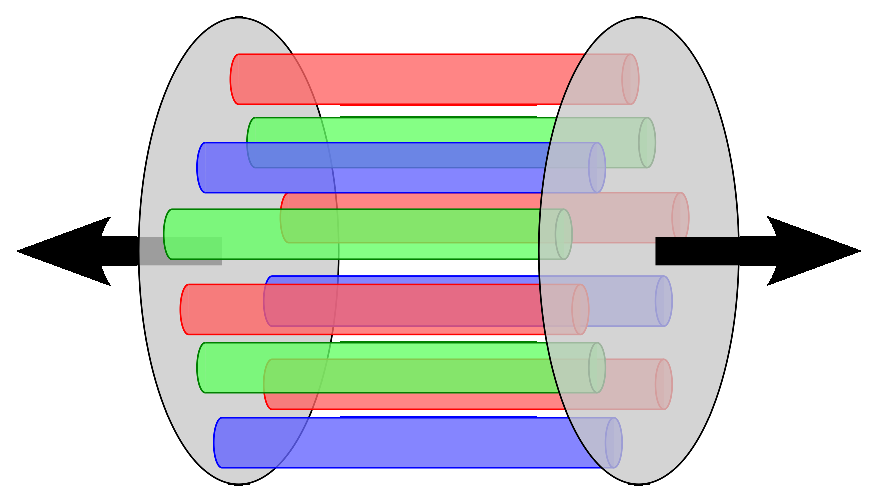
\includegraphics[width=0.9\textwidth]{images/glasma.eps}
%             \end{figure}
%         \end{center}

%        \column{.025\textwidth}
%        \column{.3\textwidth}
%         \begin{center}
%             \begin{figure}
%                 \centering
%                 \hspace{-5pt}\includegraphics[width=0.9\textwidth]{images/components.eps}
%             \end{figure}
%         \end{center}

%         \column{.025\textwidth}
%         \column{.3\textwidth}
%         \begin{center}
%             \begin{figure}
%                 \centering
%                 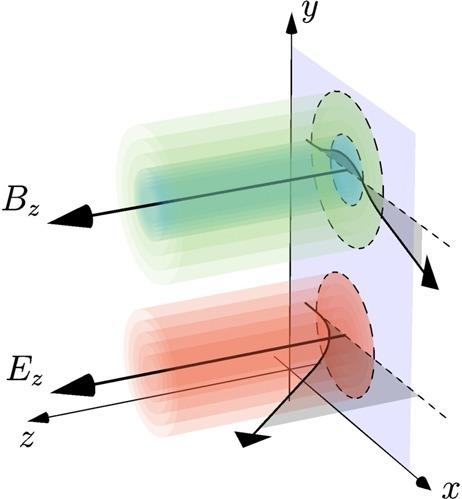
\includegraphics[width=0.7\textwidth]{images/1-s2.0-S0370269320306134-gr003_lrg.jpg}
%             \end{figure}
%         \end{center}

%         \column{.05\textwidth}
%     \end{columns}
%     \blfootnote{\scriptsize Fukushima \href{https://arxiv.org/abs/1603.02340}{{\color{palteal}\texttt{[1603.02340]}$^\text{\tiny\faExternalLink}$}}, Lappi \href{https://arxiv.org/abs/hep-ph/0606207}{{\color{palviolet}\texttt{[hep-ph/0606207]}$^\text{\tiny\faExternalLink}$}}, Ipp, Müller, Schuh \href{https://arxiv.org/abs/2009.14206}{{\color{palgold}\texttt{[2009.14206]}$^\text{\tiny\faExternalLink}$}}
%     }
% \end{frame}


% \begin{frame}
%     \frametitle{Features of the glasma}
%     \framesubtitle{Energy density profiles}
%     \begin{figure}
%         \centering
%         \includegraphics[width=0.9\textwidth]{images/flux_tubes_auau_200_nums_1_dpi_300_nounits.png}
%         \captionsetup{justification=centering}
%         \caption{Relevant scale ${\color{custompink}Q_s}$ \\
%         {\scriptsize\itshape Fields {\color{customgreen}dilute} after $\delta\tau\simeq {\color{custompink}Q}^{-1}_{\color{custompink}s}$, arrange themselves in {\color{customgreen}correlation domains} of $\delta x_T \simeq {\color{custompink}Q}^{-1}_{\color{custompink}s}$} 
%         }
%     \end{figure}
% \end{frame}

% \begin{frame}[noframenumbering]
%     \frametitle{Features of the glasma}
%     \framesubtitle{Correlation domains}
%     {\transparent{0.1}\begin{figure}
%         \centering
%         \includegraphics[width=0.9\textwidth]{images/flux_tubes_auau_200_nums_1_dpi_300_nounits.png}
%         \captionsetup{justification=centering}
%         \caption{Relevant scale ${\color{custompink}Q_s}$ \\
%         {\scriptsize\itshape Fields {\color{customgreen}dilute} after $\delta\tau\simeq {\color{custompink}Q}^{-1}_{\color{custompink}s}$, arrange themselves in {\color{customgreen}correlation domains} of $\delta x_T \simeq {\color{custompink}Q}^{-1}_{\color{custompink}s}$} 
%         }
%     \end{figure}}
%     \vspace{0.3cm}
%     \begin{center}
%         \begin{tikzpicture}[remember picture,overlay]
%             \node[align=center] at (0,4) {
%                 The fields arrange themselves in {\color{customgreen}correlation domains} of $\delta x_T \simeq {\color{custompink}Q}^{-1}_{\color{custompink}s}$\\[-5pt]
%                 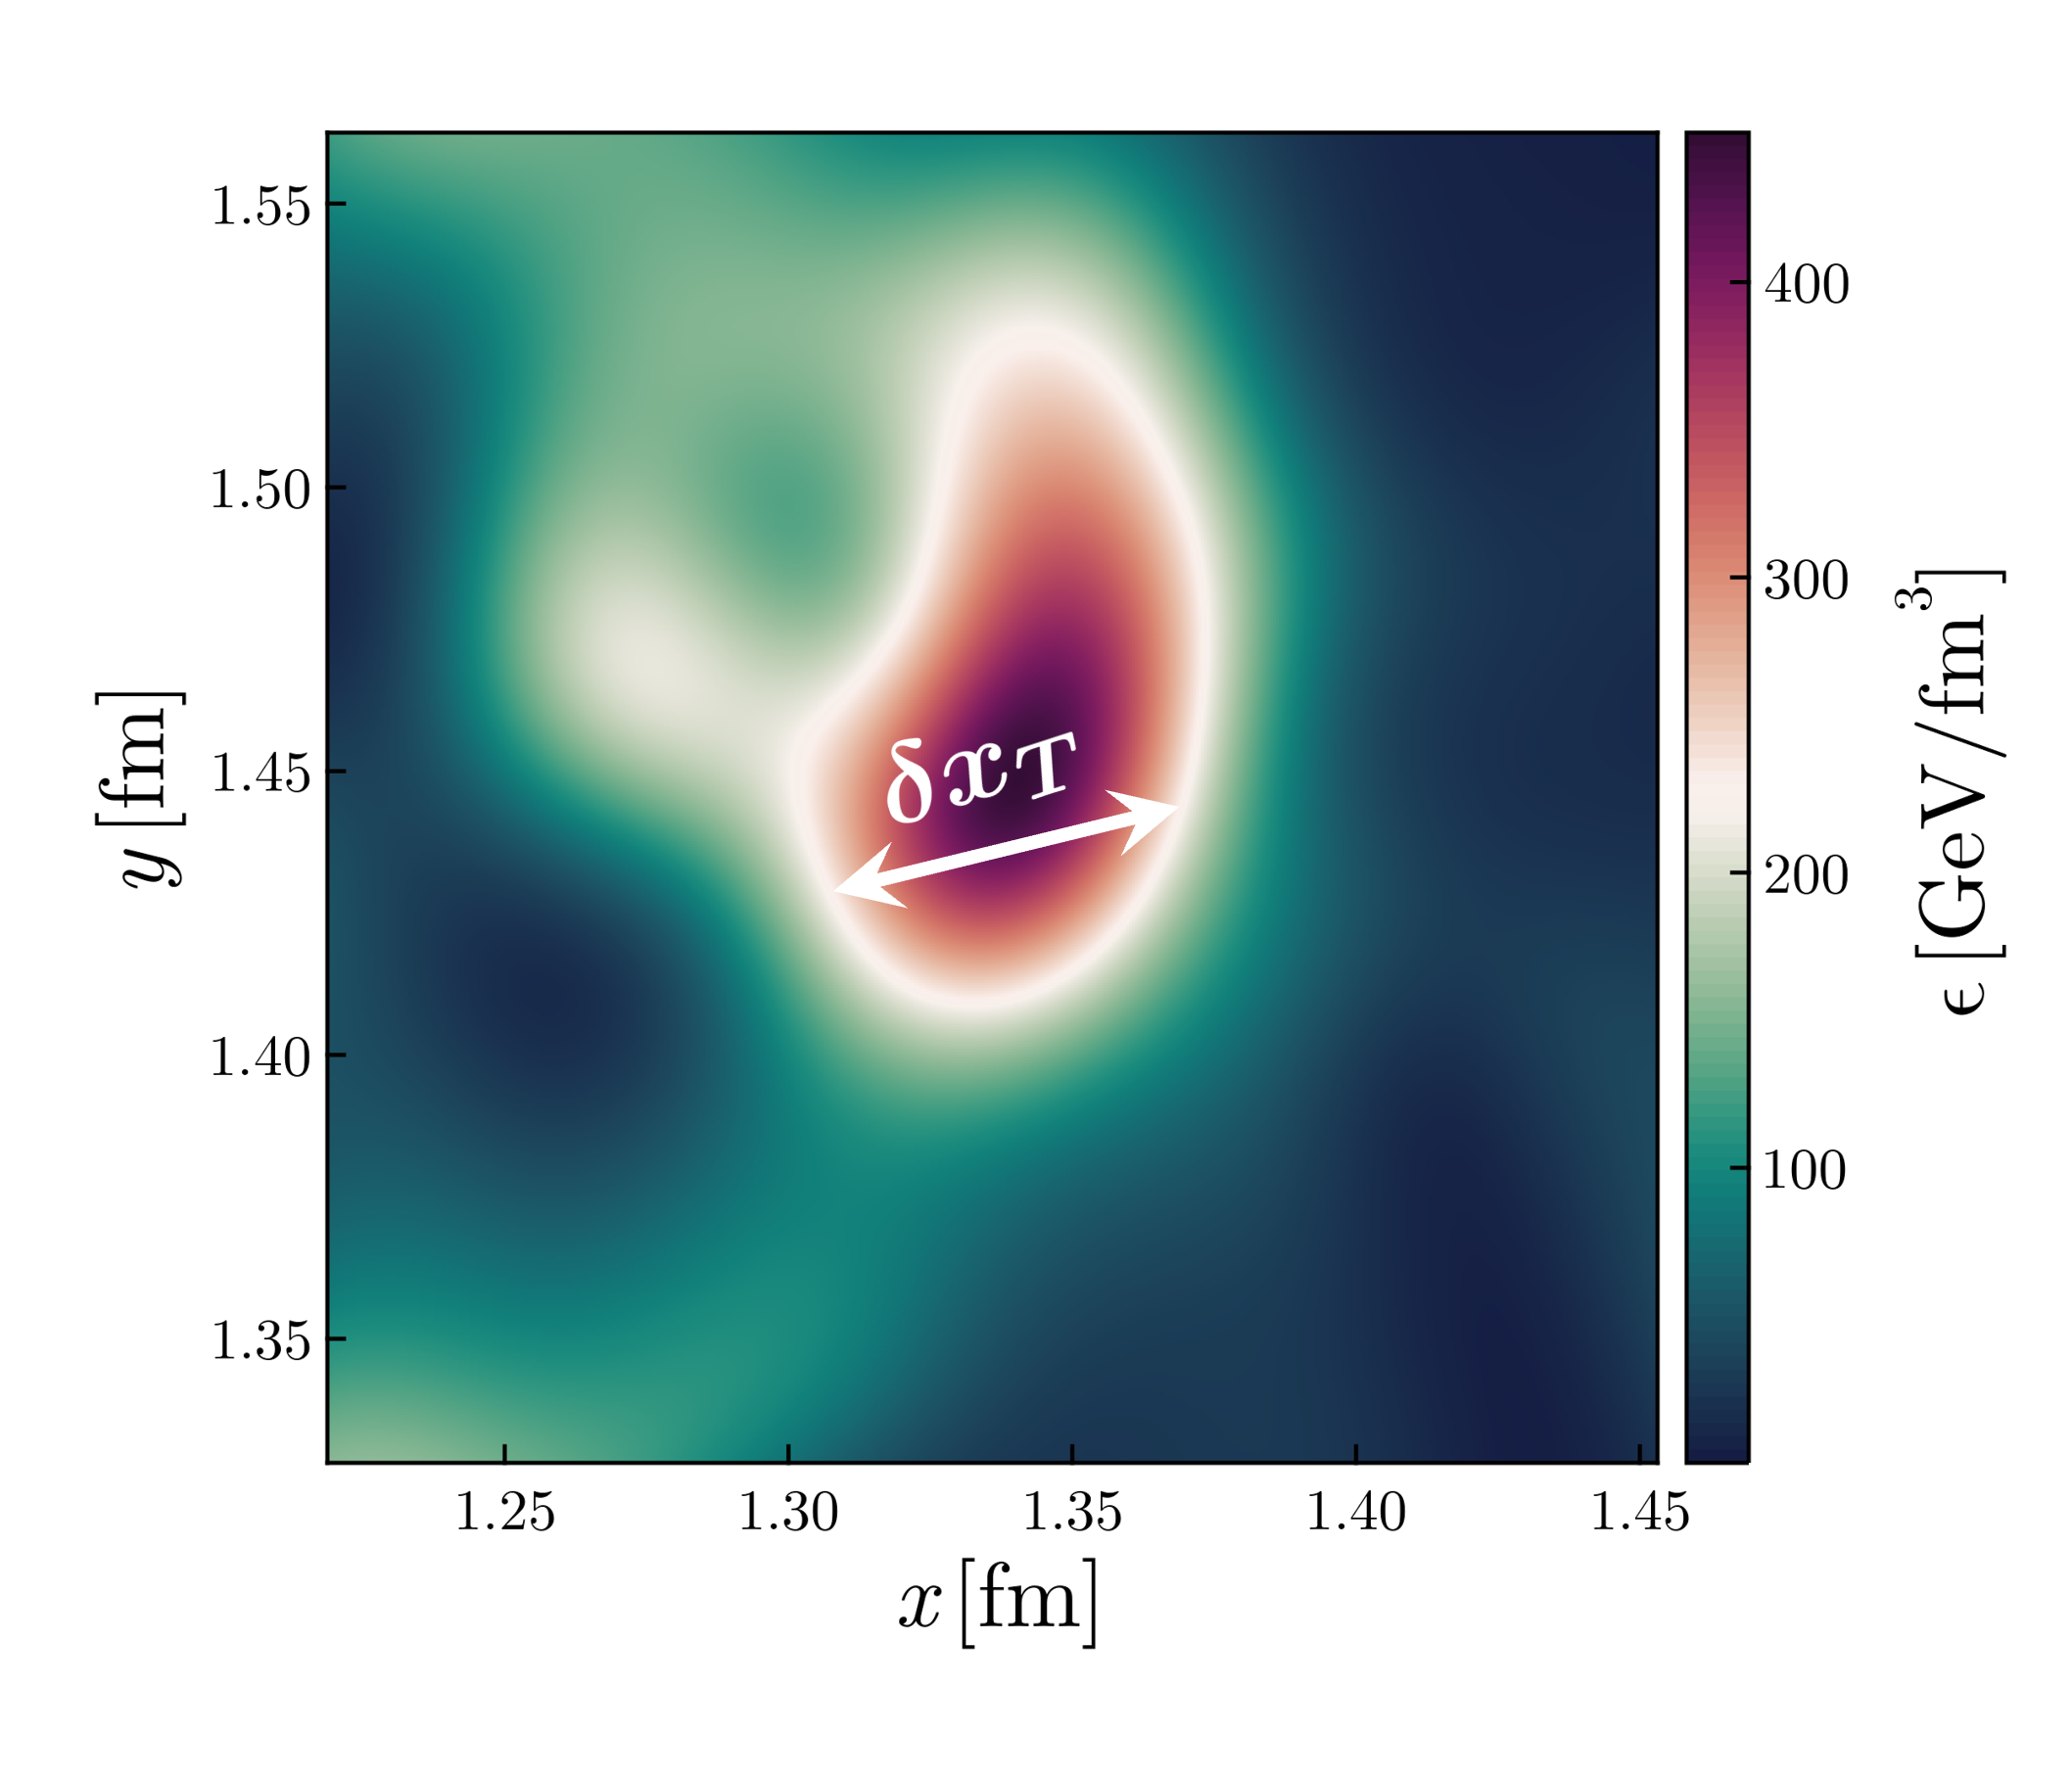
\includegraphics[width=0.48\textwidth]{images/correlation_2.png}
%             };
%         \end{tikzpicture} 
%     \end{center}
% \end{frame}

% \begin{frame}[noframenumbering]
%     \frametitle{Features of the glasma}
%     \framesubtitle{Bjorken expansion}
%     {\transparent{0.1}\begin{figure}
%         \centering
%         \includegraphics[width=0.9\textwidth]{images/flux_tubes_auau_200_nums_1_dpi_300_nounits.png}
%         \captionsetup{justification=centering}
%         \caption{Relevant scale ${\color{custompink}Q_s}$ \\
%         {\scriptsize\itshape Fields {\color{customgreen}dilute} after $\delta\tau\simeq {\color{custompink}Q}^{-1}_{\color{custompink}s}$, arrange themselves in {\color{customgreen}correlation domains} of $\delta x_T \simeq {\color{custompink}Q}^{-1}_{\color{custompink}s}$} 
%         }
%     \end{figure}}
%     \begin{center}
%         \begin{tikzpicture}[remember picture,overlay]
%             \node[align=center] at (0,4) {
%                 The fields become {\color{customgreen}dilute} after $\delta\tau\simeq {\color{custompink}Q}^{-1}_{\color{custompink}s}$\\
%                 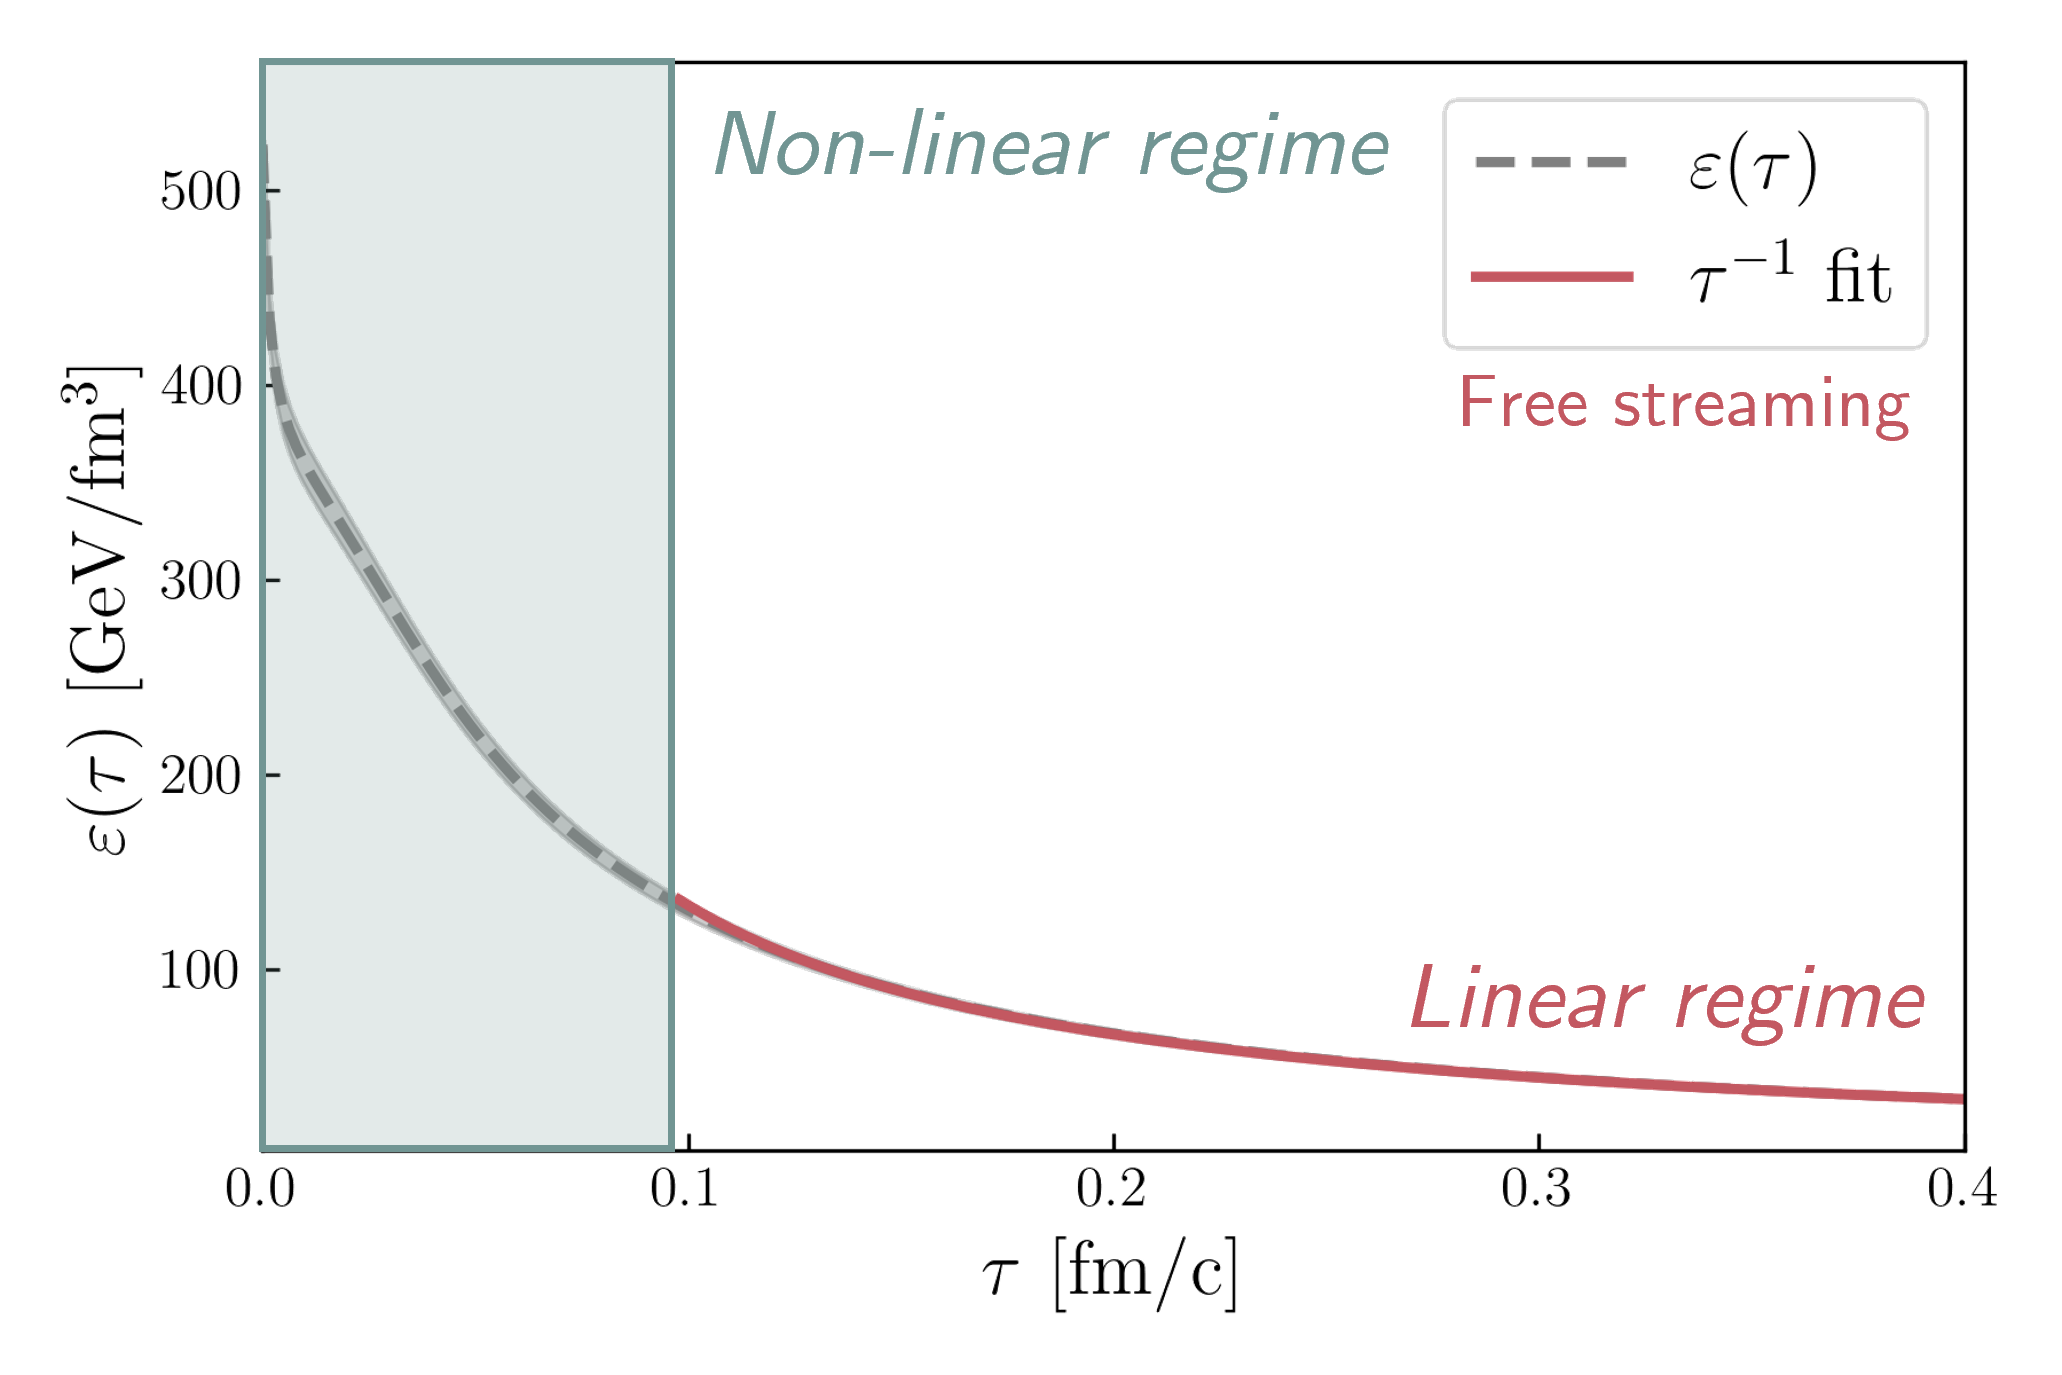
\includegraphics[width=0.55\textwidth]{images/dilute_2.png}
%             };
%         \end{tikzpicture} 
%     \end{center}
% \end{frame}



% \begin{frame}[noframenumbering]
%     \frametitle{Features of the glasma}
%     \framesubtitle{Anisotropic fields}
%     {\transparent{0.1}\begin{figure}
%         \centering
%         \includegraphics[width=0.9\textwidth]{images/flux_tubes_auau_200_nums_1_dpi_300_nounits.png}
%         \captionsetup{justification=centering}
%         \caption{Relevant scale ${\color{custompink}Q_s}$ \\
%         {\scriptsize\itshape Fields {\color{customgreen}dilute} after $\delta\tau\simeq {\color{custompink}Q}^{-1}_{\color{custompink}s}$, arrange themselves in {\color{customgreen}correlation domains} of $\delta x_T \simeq {\color{custompink}Q}^{-1}_{\color{custompink}s}$} 
%         }
%     \end{figure}}
%     \vspace{0.3cm}
%     \begin{center}
%         \begin{tikzpicture}[remember picture,overlay]
%             \node[align=center] at (0,4) {
%                 Longitudinal $\neq$ transverse $\Rightarrow$ {\color{pinky}anisotropy}\\
%                 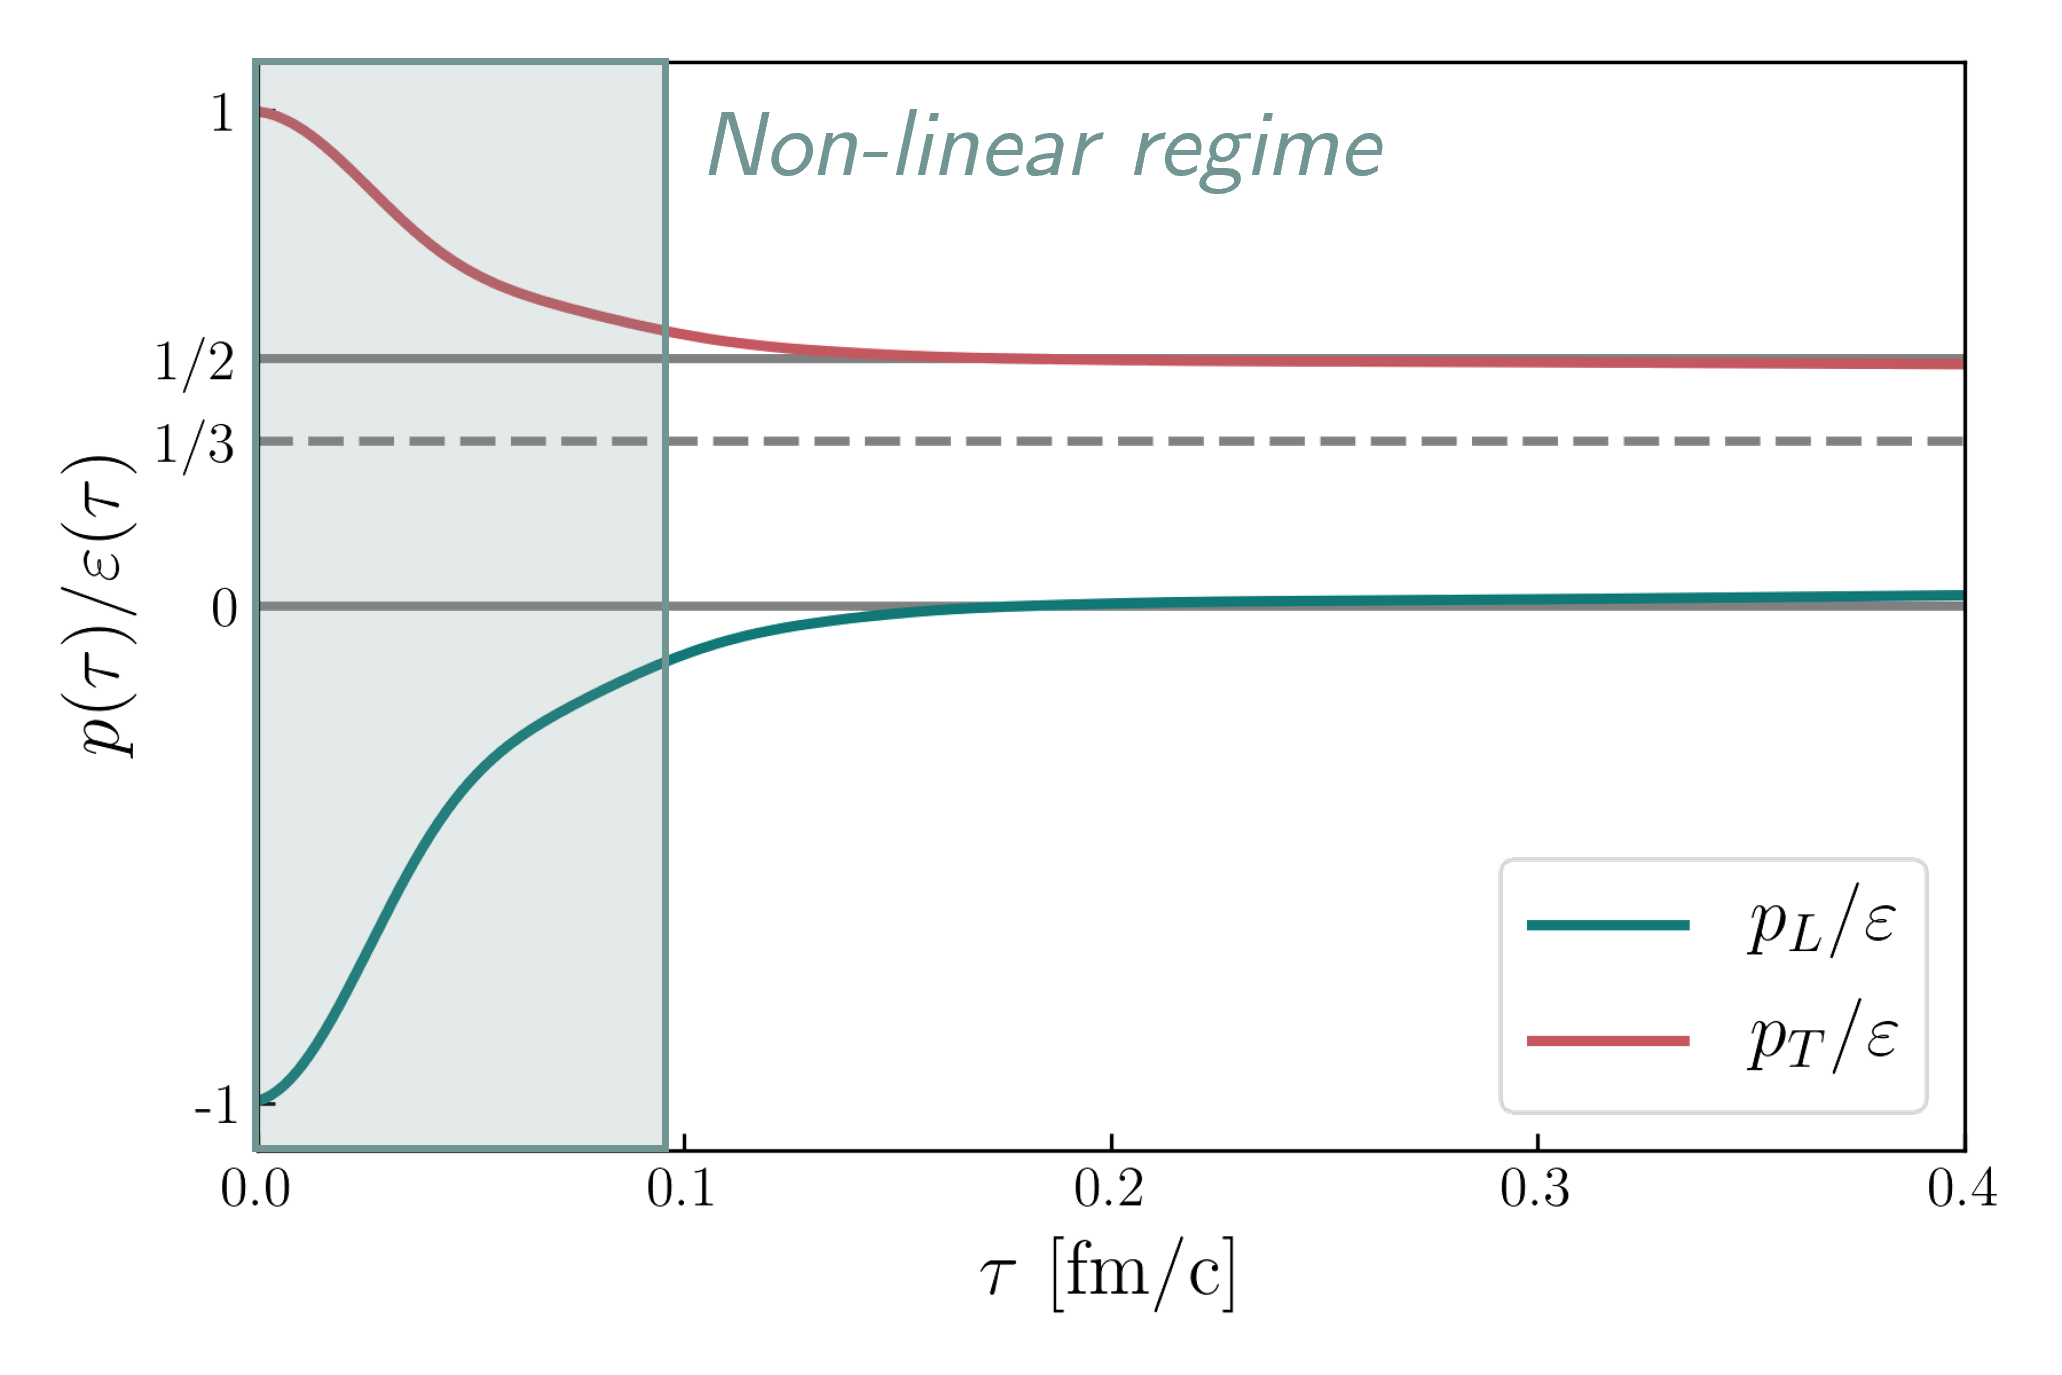
\includegraphics[width=0.55\textwidth]{images/anisotropy.png}
%             };
%         \end{tikzpicture} 
%     \end{center}
% \end{frame}



%%%%%%%%%%%%%%%%%%%%%%%%%%%%%%%%%%%%%%%%%
%%%%%%%%%%%%%% SUBSECTION %%%%%%%%%%%%%%%
%%%%%%%%%%%%%%%%%%%%%%%%%%%%%%%%%%%%%%%%%

\subsection{Frameworks}

%%%%%%%%%%%%%%%%%%%%%%%%%%%%%%%%%%%%%%%%%
%%%%%%%%%%%%%%%%% SLIDE %%%%%%%%%%%%%%%%%
%%%%%%%%%%%%%%%%%%%%%%%%%%%%%%%%%%%%%%%%%

\begin{frame}
    \frametitle{Frameworks for glasma}
    \framesubtitle{Analytical approaches, 3+1D extensions}
\end{frame}



%%%%%%%%%%%%%%%%%%%%%%%%%%%%%%%%%%%%%%%%%
%%%%%%%%%%%%%%%% SECTION %%%%%%%%%%%%%%%%
%%%%%%%%%%%%%%%%%%%%%%%%%%%%%%%%%%%%%%%%%

\section{Transport in glasma}


%%%%%%%%%%%%%%%%%%%%%%%%%%%%%%%%%%%%%%%%%
%%%%%%%%%%%%%%%%% SLIDE %%%%%%%%%%%%%%%%%
%%%%%%%%%%%%%%%%%%%%%%%%%%%%%%%%%%%%%%%%%

\setbeamertemplate{background}{
\tikz[overlay,remember picture] \node[opacity=0.1, at=(current page.center), align=center] {\\[10pt]
{\transparent{0.1}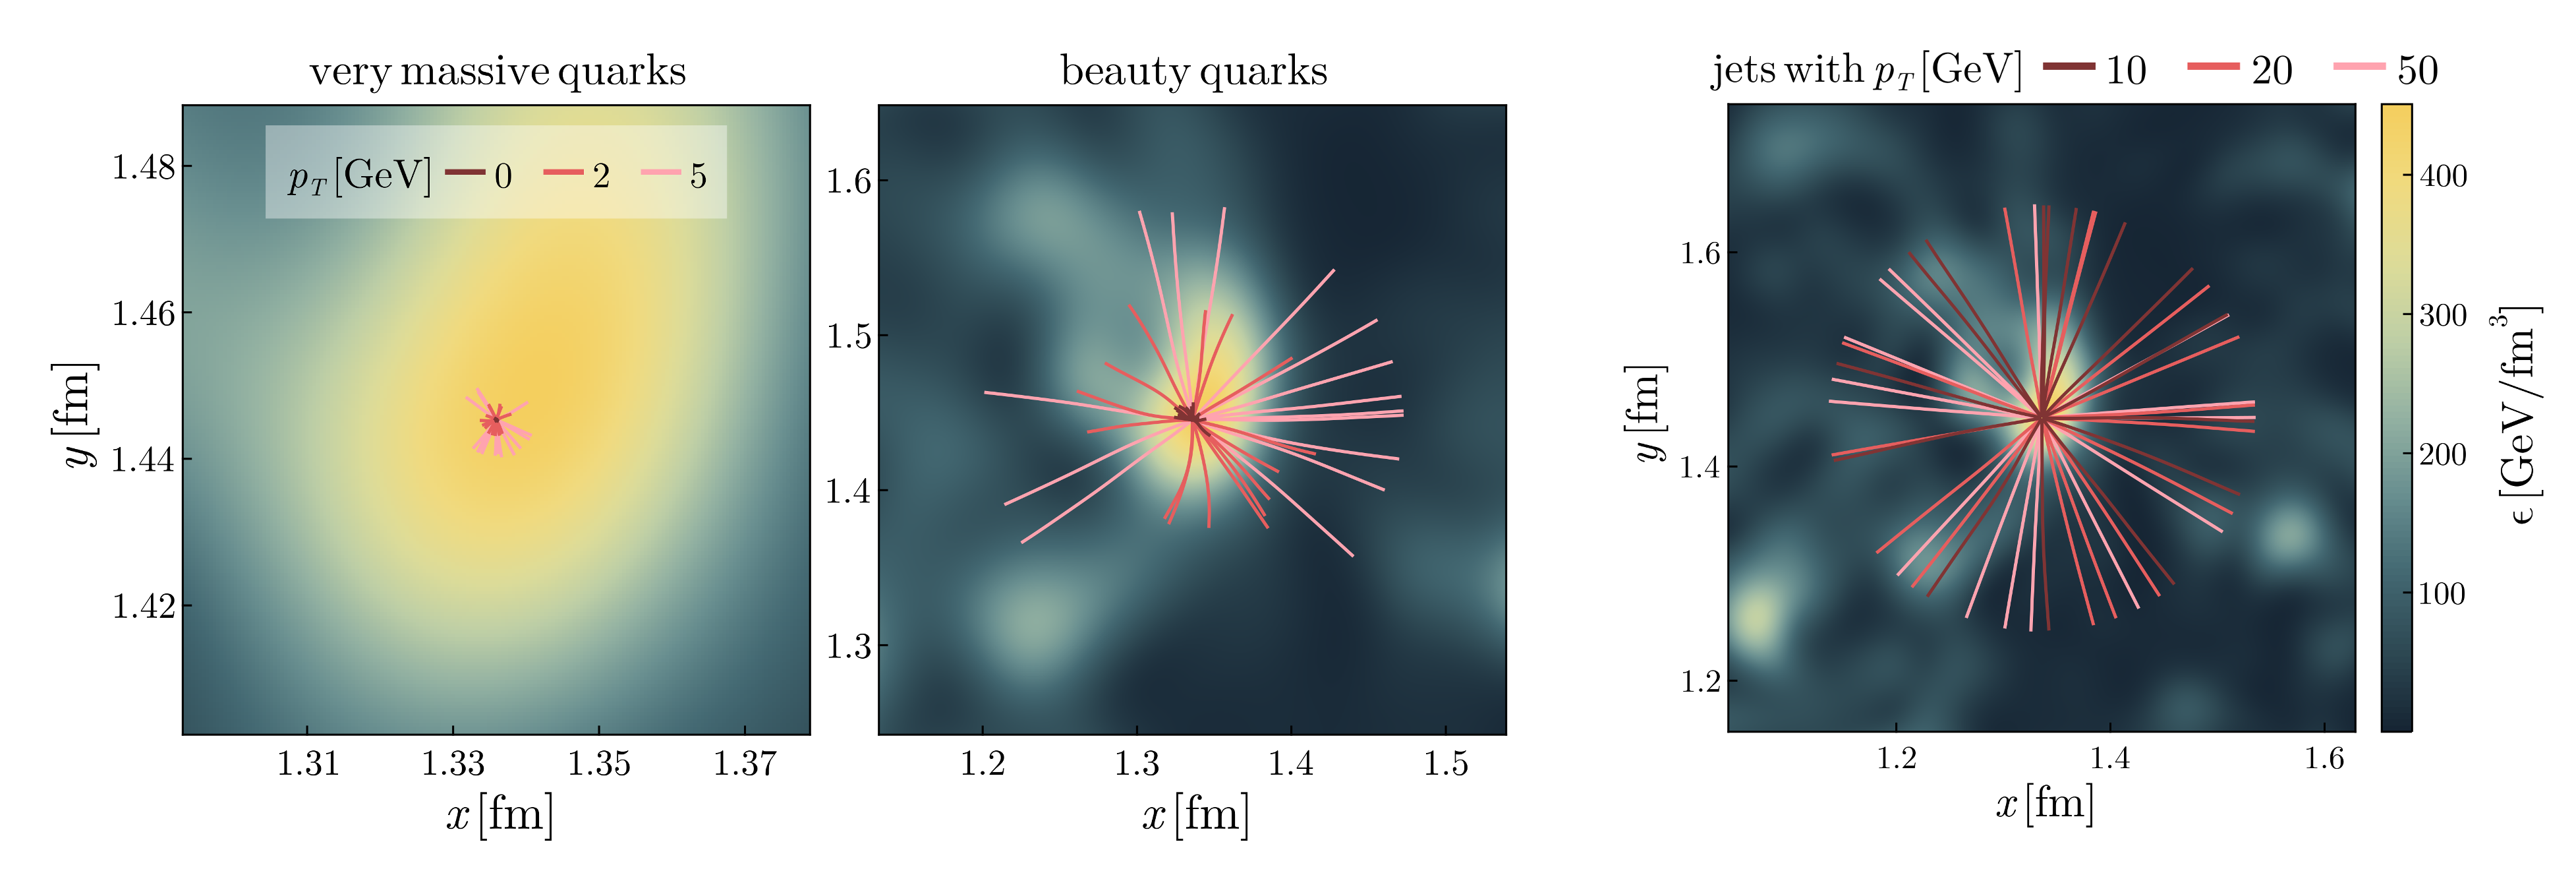
\includegraphics[width=\paperwidth]{images/hqs_jets_trajectories.png}}};
}
\setbeamertemplate{itemize item}{\raisebox{0.2em}{\scalebox{0.7}{${\color{normal}\blacktriangleright}$}}} 
\begin{frame}[plain,noframenumbering]{}
    \begin{center}
        \vspace{1cm}
        {\large\color{normal}Transport during pre-equilibrium}\\[0.3cm]
        {\huge\color{destacado}Hard probes in glasma}\\[0.3cm]
    \end{center}
\end{frame}
\setbeamertemplate{background}{}

%%%%%%%%%%%%%%%%%%%%%%%%%%%%%%%%%%%%%%%%%
%%%%%%%%%%%%%%%%% SLIDE %%%%%%%%%%%%%%%%%
%%%%%%%%%%%%%%%%%%%%%%%%%%%%%%%%%%%%%%%%%

\setbeamertemplate{background}{
\tikz[overlay,remember picture] \node[at=(current page.center), align=center] {\\[20pt]
{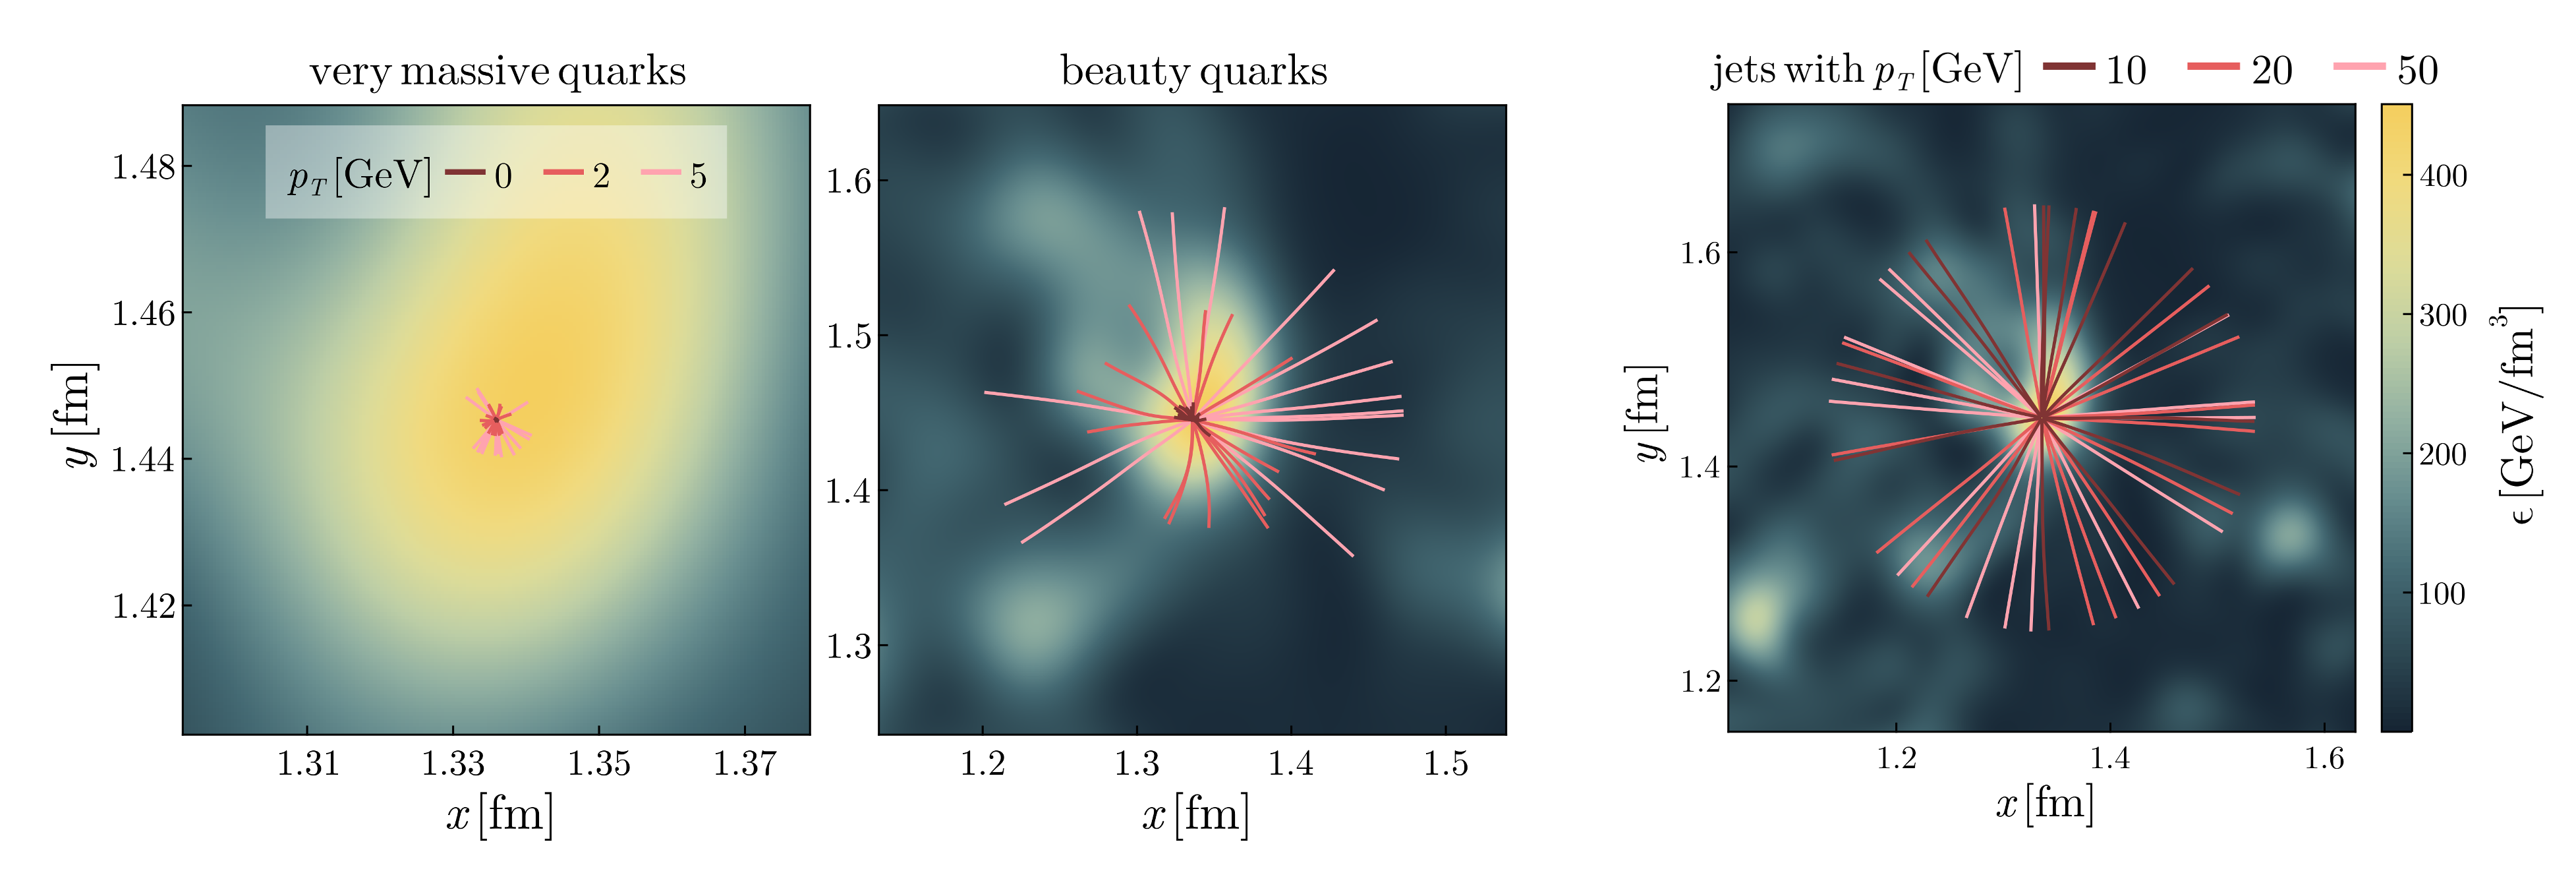
\includegraphics[width=\paperwidth]{images/hqs_jets_trajectories.png}}};
}
\setbeamertemplate{itemize item}{\raisebox{0.2em}{\scalebox{0.7}{${\color{normal}\blacktriangleright}$}}} 
\begin{frame}[plain, noframenumbering]
    \frametitle{\\ Heavy quarks and jet in glasma}
    \framesubtitle{Probing the glasma fields}
    \blfootnote{\scriptsize Avramescu, Băran, Greco, Ipp, Müller, Ruggieri  \href{https://arxiv.org/abs/2303.05599}{{\color{palgold}\texttt{[2303.05599]}$^\text{\tiny\faExternalLink}$}}}
\end{frame}
\setbeamertemplate{background}{}


%%%%%%%%%%%%%%%%%%%%%%%%%%%%%%%%%%%%%%%%%
%%%%%%%%%%%%%% SUBSECTION %%%%%%%%%%%%%%%
%%%%%%%%%%%%%%%%%%%%%%%%%%%%%%%%%%%%%%%%%

\subsection{Classical transport}

% %%%%%%%%%%%%%%%%%%%%%%%%%%%%%%%%%%%%%%%%%
% %%%%%%%%%%%%%%%%% SLIDE %%%%%%%%%%%%%%%%%
% %%%%%%%%%%%%%%%%%%%%%%%%%%%%%%%%%%%%%%%%%

\begin{frame}
    \frametitle{Particles in Yang-Mills fields}
    \framesubtitle{Wong's equations of motion}
        \setbeamertemplate{itemize item}{\raisebox{0.2em}{\scalebox{0.7}{${\color{ming}\blacktriangleright}$}}} 
   \begin{center}
    \begin{custombox2}{Classical transport equations}{lightgray}
        \small
        \begin{varwidth}{0.75\textwidth}
        \begin{itemize}\itemsep0em 
            \setbeamertemplate{itemize item}{\raisebox{0.2em}{\scalebox{0.7}{${\color{lightgray}\blacktriangleright}$}}} 
            \item \begin{center}Wong's equations $\leftrightarrow$ classical equations of motion for particles\\
            $({\color{customblue}x^\mu},{\color{customred}p^\mu},{\color{customyellow}Q})$ evolving in a Yang-Mills background field ${\color{starrysecond}A^\mu}$\end{center} 
        \end{itemize}
        \end{varwidth}
    \end{custombox2}

    %    Wong's equations $\leftrightarrow$ classical equations of motion for particles $({\color{customblue}x^\mu},{\color{customred}p^\mu},{\color{customyellow}Q})$ \\
    % evolving in a Yang-Mills background field ${\color{starrysecond}A^\mu}$
   \end{center} 
        \vspace{1cm}
        \renewcommand{\eqnhighlightheight}{\vphantom{x}}
        \begin{equation*}
            \frac{\d}{\d\hspace{-0.1cm}\eqnmark[destacado]{tau}{\boldsymbol{\tau}}\hspace{-0.2cm}}\eqnmark[customblue]{xmu}{x^\mu}=\frac{{\color{customred}p^\mu}}{\eqnmark[destacado]{m}{m}},\qquad \frac{\mathrm{d}}{\d\boldsymbol{\tau}}\hspace{-0.1cm}\eqnmark[customred]{pmu}{p^\mu}=\eqnmark[destacado]{tr}{\dfrac{1}{\color{lightgray}T_R}}\hspace{-0.1cm}\eqnmark[destacado]{g}{g}\tr{{\color{customyellow}Q}F^{\mu\nu}[\hspace{-0.1cm}\eqnmark[starrysecond]{amu}{A^\mu}\hspace{-0.1cm}]}\frac{{\color{customred}p_\nu}}{m},\qquad 
            \underbrace{\frac{\d}{\d\boldsymbol{\tau}}\hspace{-0.1cm}\eqnmark[customyellow]{Q}{Q}\hspace{-0.1cm}=-\mathrm{i}g [{\color{starrysecond}A_\mu},{\color{customyellow}Q}]\,\frac{{\color{customred}p^\mu}}{m}}_{\substack{\text{\footnotesize color rotation}\,\rightarrow\,{\color{customgreen}\mathcal{U}}\in\,\mathrm{SU(3)} \\[0.2cm] {\color{customyellow}Q}(\boldsymbol{\tau})=\,{\color{customgreen}\mathcal{U}}(\boldsymbol{\tau},\boldsymbol{\tau}^\prime){\color{customyellow}Q}(\boldsymbol{\tau^\prime})\,{\color{customgreen}\mathcal{U}^\dagger}(\boldsymbol{\tau},\boldsymbol{\tau}^\prime)}}
            \end{equation*}
            \annotate[yshift=1.2em]{above}{xmu}{coordinate}
            \annotate[yshift=1.2em]{above}{pmu}{momentum}
            \annotate[yshift=-0.5em]{below, right}{m}{\tiny mass}
            % \annotate[yshift=-1.5em]{below, right}{Ddtau}{\tiny covariant derivative}
            \annotate[yshift=-1.5em]{below, right}{tr}{\tiny\color{lightgray} $\mathrm{Tr}\{T^aT^b\}=T_R\delta^{ab}$}
            \annotate[yshift=-1.5em]{below, right}{tau}{\tiny proper time}
            \annotate[yshift=-0.7em]{below, right}{g}{\tiny coupling constant}
            \annotate[yshift=1.2em]{above}{Q}{color charge}
            \annotate[yshift=1.2em]{above, right}{amu}{gauge field}

    \begin{itemize}\itemsep0em 
        \setbeamertemplate{itemize item}{\raisebox{0.1em}{\scalebox{0.7}{${\color{starrysecond}\blacktriangleright}$}}} 
        \item \begin{center}\footnotesize Solve the classical transport equations with {\color{starrysecond}$A^\mu$} the {\color{starrysecond}glasma field}\end{center} 
        \setbeamertemplate{itemize item}{\raisebox{0.1em}{\scalebox{0.7}{${\color{palgold}\blacktriangleright}$}}} 
        \item \begin{center}\footnotesize Color rotation conserves ${\color{palgold}q_{2}}=Q^aQ^a$ and ${\color{palgold}q_3}=d_{abc}Q^aQ^bQ^c$ {\color{palgold}SU($3$) Casimir invariants} \end{center} 
    \end{itemize}
\end{frame}


%%%%%%%%%%%%%%%%%%%%%%%%%%%%%%%%%%%%%%%%%
%%%%%%%%%%%%%%%%% SLIDE %%%%%%%%%%%%%%%%%
%%%%%%%%%%%%%%%%%%%%%%%%%%%%%%%%%%%%%%%%%

\begin{frame}
    \frametitle{Particles in glasma fields}
    \framesubtitle{Visualizing the trajectories}
    \vspace{-0.5cm}
    \begin{columns}[onlytextwidth,t]
        \column{.025\textwidth}
       \column{.3\textwidth}
            \begin{itemize}\itemsep0em 
                \setbeamertemplate{itemize item}{\raisebox{0.2em}{\scalebox{0.7}{${\color{normal}\blacktriangleright}$}}} 
                \item \begin{center}\footnotesize Change in {\bfseries coordinates} due to momentum kicks\end{center}
            \end{itemize}
                \vspace{-20pt}
                \begin{figure}[!hbt]
                    \centering
                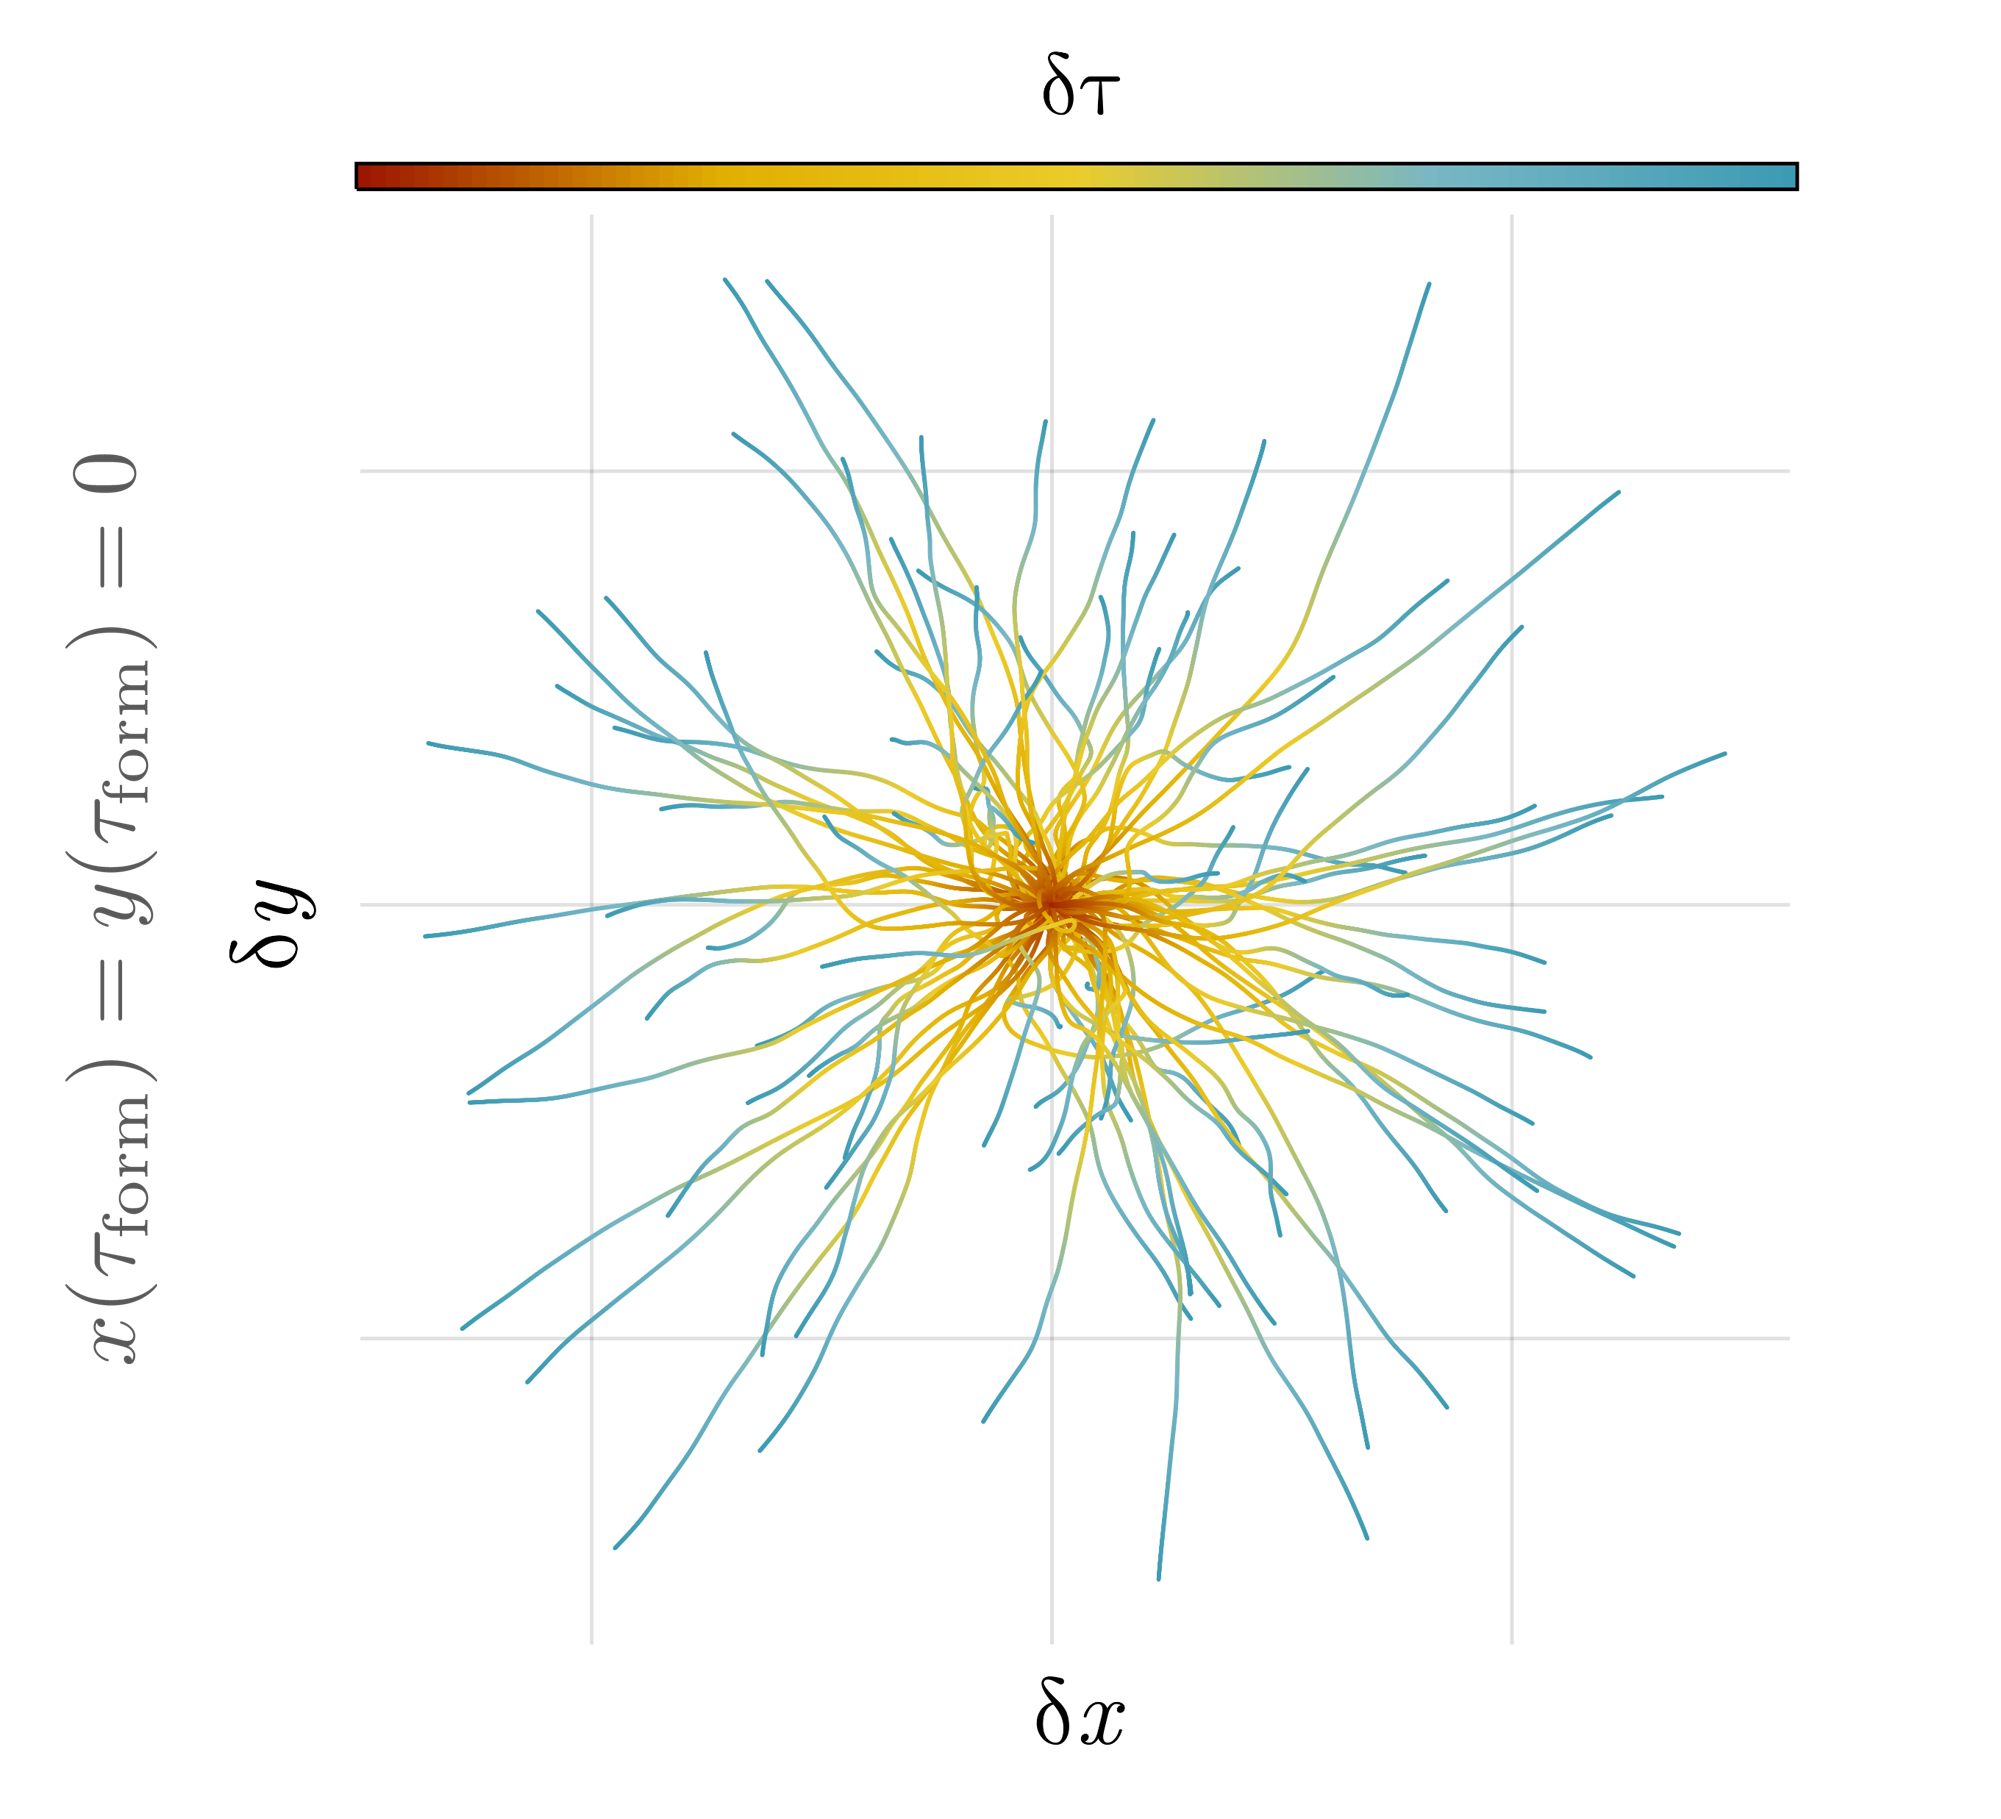
\includegraphics[width=1.1\columnwidth]{images/wong_coord.png}
                \end{figure}
                \column{.025\textwidth}
        \column{.3\textwidth}
            \begin{itemize}\itemsep0em 
                \setbeamertemplate{itemize item}{\raisebox{0.2em}{\scalebox{0.7}{${\color{normal}\blacktriangleright}$}}} 
                \item \begin{center}\footnotesize {\bfseries Momentum} broadening due to color Lorentz force\end{center}
            \end{itemize}
            \vspace{-20pt}
            \begin{figure}[!hbt]
                \centering
                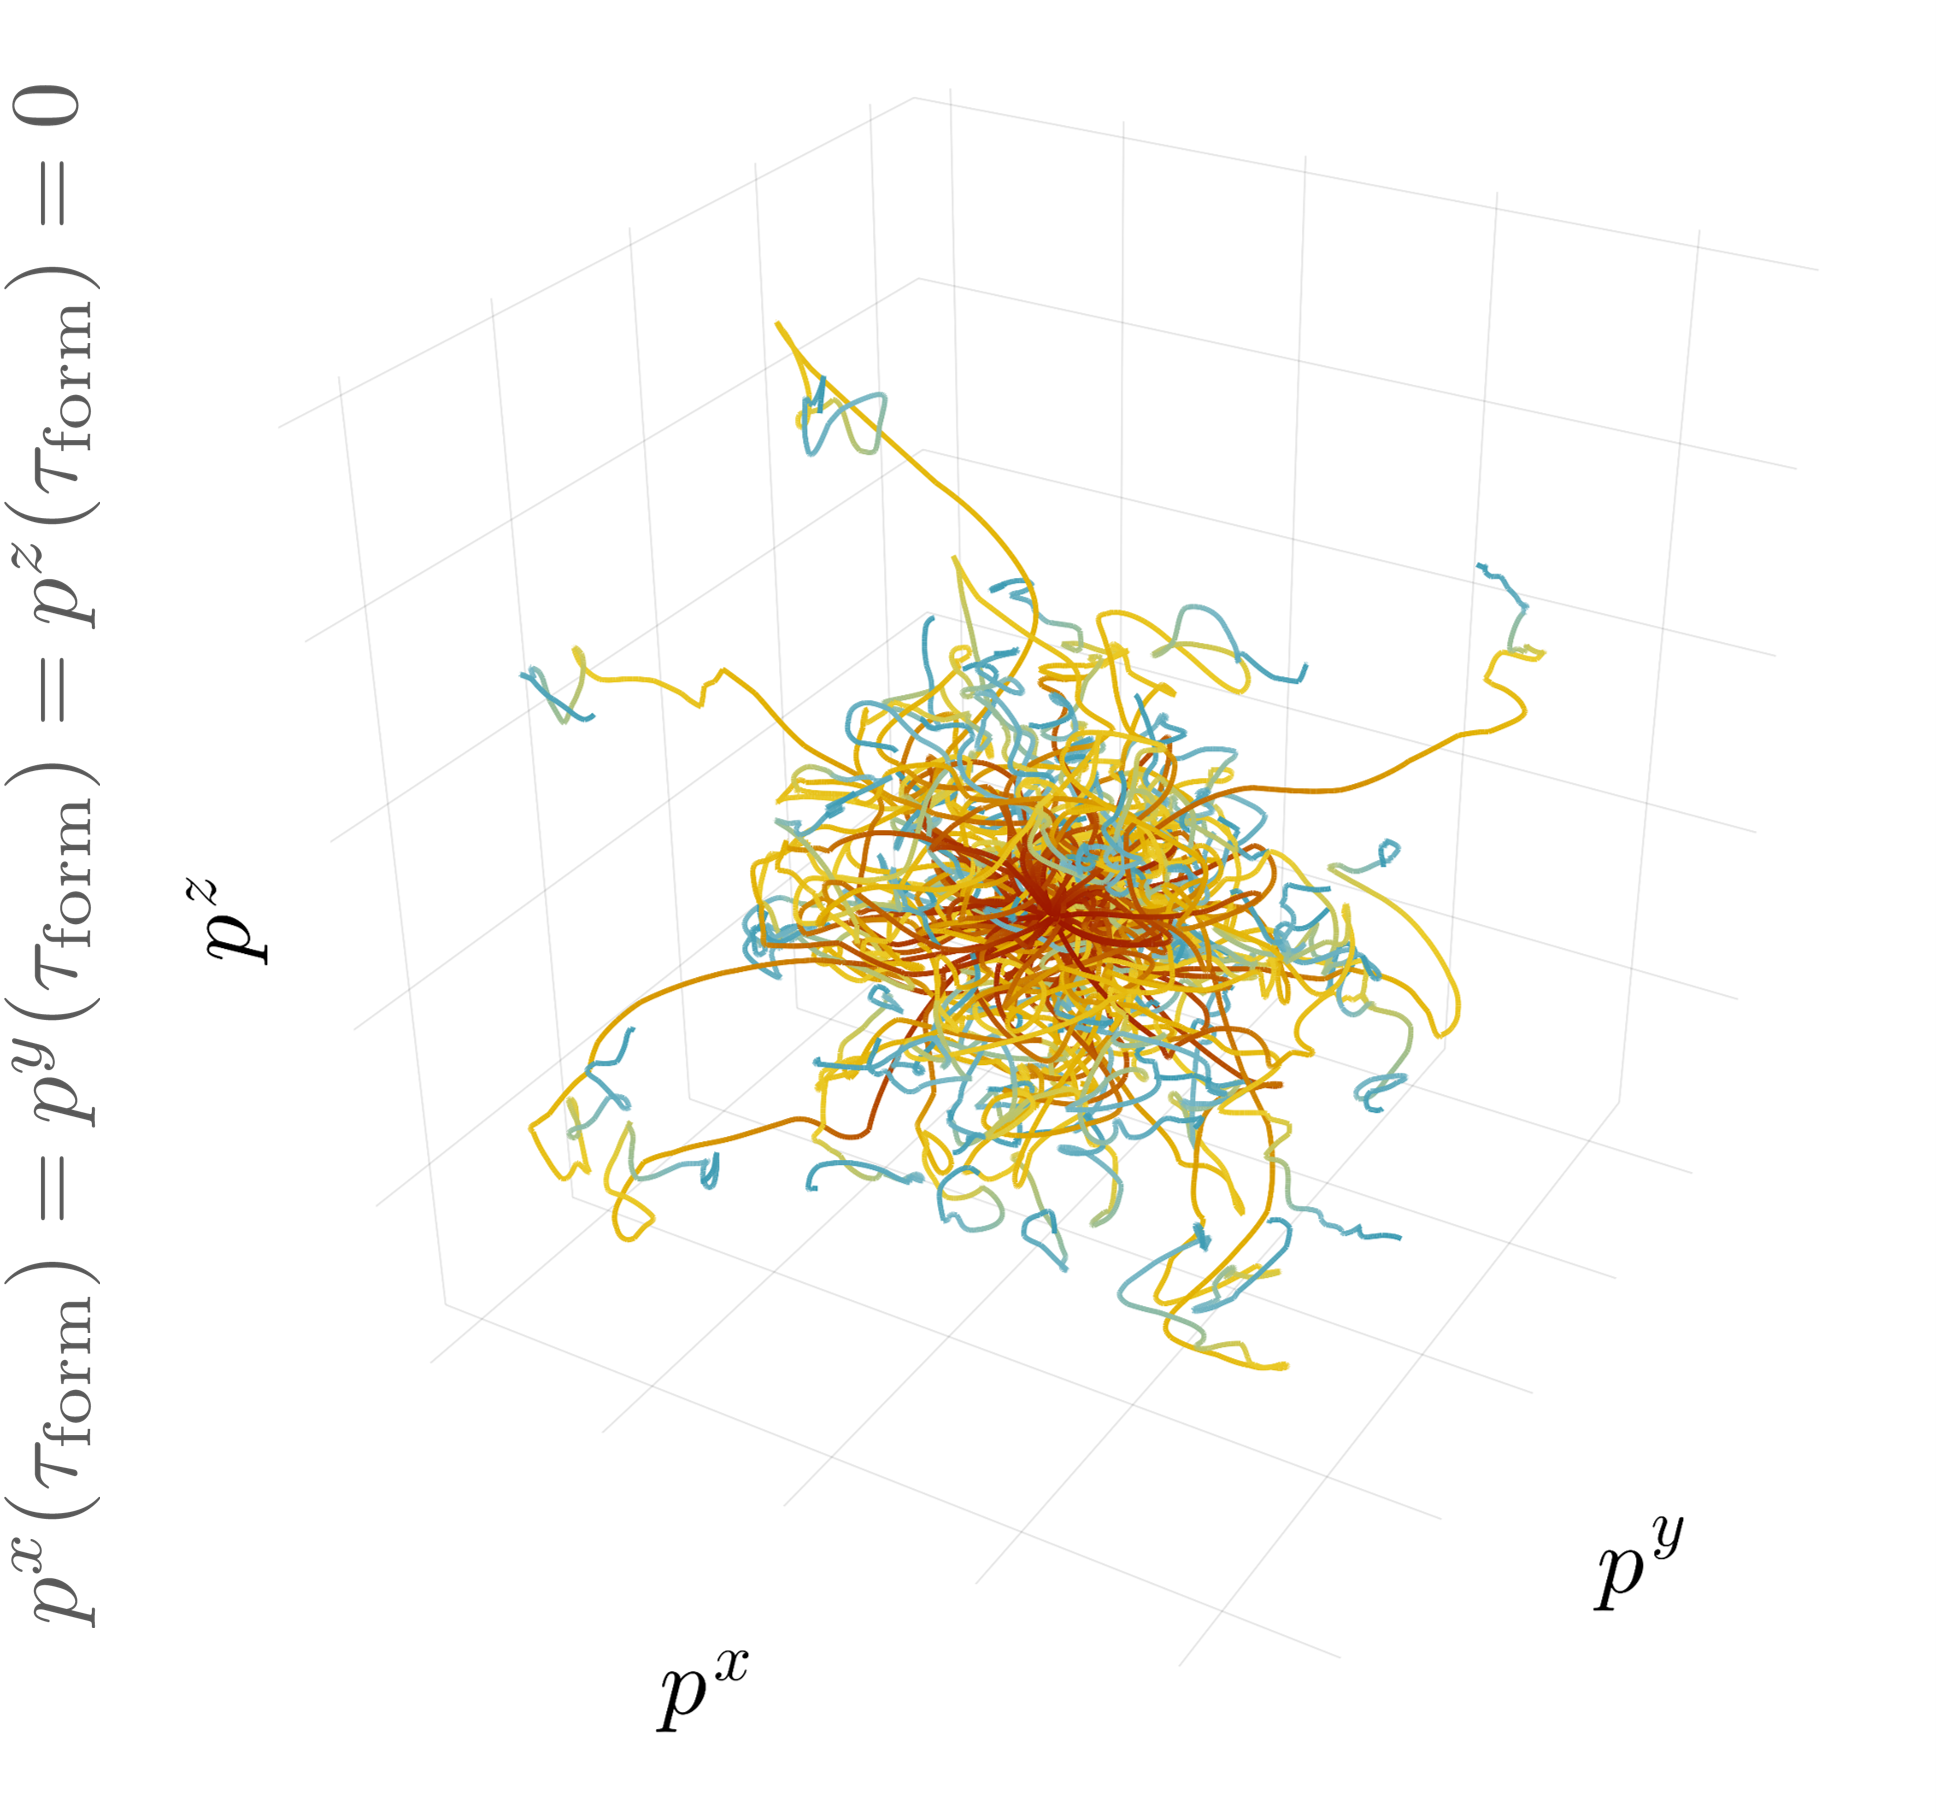
\includegraphics[width=1.1\columnwidth]{images/wong_mom.png}
            \end{figure}
            \column{.025\textwidth}
        \column{.3\textwidth}
            \begin{itemize}\itemsep0em 
                \setbeamertemplate{itemize item}{\raisebox{0.2em}{\scalebox{0.7}{${\color{normal}\blacktriangleright}$}}} 
                \item \begin{center}\footnotesize {\bfseries Color charge} rotation in SU(3) with Wilson lines\end{center}
            \end{itemize}
            \vspace{-15pt}
            \begin{figure}[!hbt]
                \centering
                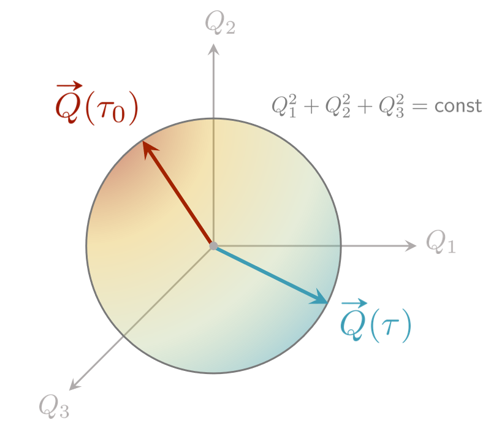
\includegraphics[width=1.05\columnwidth]{images/wong_charge.png}
            \end{figure}
            \column{.025\textwidth}
    \end{columns}

    \blfootnote{\scriptsize Avramescu, Băran, Greco, Ipp, Müller, Ruggieri  \href{https://arxiv.org/abs/2303.05599}{{\color{palgold}\texttt{[2303.05599]}$^\text{\tiny\faExternalLink}$}}}
\end{frame}



% %%%%%%%%%%%%%%%%%%%%%%%%%%%%%%%%%%%%%%%%%
% %%%%%%%%%%%%%%%%% SLIDE %%%%%%%%%%%%%%%%%
% %%%%%%%%%%%%%%%%%%%%%%%%%%%%%%%%%%%%%%%%%

\begin{frame}
    \frametitle{Colored Particle-in-Cell}
    \framesubtitle{Boltzmann-Vlasov equations}
        \setbeamertemplate{itemize item}{\raisebox{0.2em}{\scalebox{0.7}{${\color{ming}\blacktriangleright}$}}} 
   \begin{center}
    \begin{custombox2}{Classical transport equations}{lightgray}
        \small
        \begin{varwidth}{0.82\textwidth}
        \begin{itemize}\itemsep0em 
            \setbeamertemplate{itemize item}{\raisebox{0.2em}{\scalebox{0.7}{${\color{lightgray}\blacktriangleright}$}}} 
            \item \begin{center}Wong's equations $\leftrightarrow$ equations of motion for test particles $({\color{customblue}x^\mu},{\color{customred}p^\mu},{\color{customyellow}Q})$\\
            probing a distribution function $\boldsymbol{f}({\color{customblue}x^\mu}, {\color{customred}p^\mu}, {\color{customyellow}Q^a})$ in a Yang-Mills field ${\color{starrysecond}A^\mu}$\end{center} 
        \end{itemize}
        \end{varwidth}
    \end{custombox2}

   \end{center} 
    \begin{itemize}\itemsep0em 
        \setbeamertemplate{itemize item}{\raisebox{0.1em}{\scalebox{0.7}{${\color{starrysecond}\blacktriangleright}$}}} 
        \item \begin{center} Boltzmann-Vlasov equation for {\color{red}collisionless} non-Abelian plasma\\[10pt]
            ${\color{customred}p^\mu}[\partial_\mu+g {\color{customyellow}Q^a} {\color{starrysecond}F^{\mu\nu}}({\color{customblue}x^\mu})\partial^\nu_{{\color{customred}p^\mu}}+gf^{abc}{\color{starrysecond}A^b_\mu}({\color{customblue}x^\mu}){\color{customyellow}Q^c}\partial_{{\color{customyellow}Q^a}}]\boldsymbol{f}({\color{customblue}x^\mu}, {\color{customred}p^\mu}, {\color{customyellow}Q^a})={\color{red}0}$\\[10pt]\end{center}
            \begin{center} $\boldsymbol{f}({\color{customblue}x^\mu}, {\color{customred}p^\mu}, {\color{customyellow}Q^a})\xrightarrow{\text{sample}}$ test particles $({\color{customblue}x^\mu}, {\color{customred}p^\mu}, {\color{customyellow}Q^a})\Rightarrow$ Wong's equations\\[10pt] \end{center} 
        \item \begin{center} Particle current $j^\mu\xleftrightarrow{\text{couple}}$ fields $\mathcal{D}_\mu F^{\mu\nu}[{\color{starrysecond}A^a_\mu}]=j^\mu({\color{customblue}x^\mu}, {\color{customred}p^\mu}, {\color{customyellow}Q^a})$ \end{center} 
    \end{itemize}
        

    % \begin{itemize}\itemsep0em 
    %     \setbeamertemplate{itemize item}{\raisebox{0.1em}{\scalebox{0.7}{${\color{starrysecond}\blacktriangleright}$}}} 
    %     \item \begin{center}\footnotesize Solve the classical transport equations with {\color{starrysecond}$A^\mu$} the {\color{starrysecond}glasma field}\end{center} 
    %     \setbeamertemplate{itemize item}{\raisebox{0.1em}{\scalebox{0.7}{${\color{palgold}\blacktriangleright}$}}} 
    %     \item \begin{center}\footnotesize Color rotation conserves ${\color{palgold}q_{2}}=Q^aQ^a$ and ${\color{palgold}q_3}=d_{abc}Q^aQ^bQ^c$ {\color{palgold}SU($3$) Casimir invariants} \end{center} 
    % \end{itemize}

    \blfootnote{\scriptsize Moore, Hu, Muller  \href{https://arxiv.org/abs/hep-ph/9710436}{{\color{palgold}\texttt{[hep-ph/9710436]}$^\text{\tiny\faExternalLink}$}}, Dumitru, Nara, Strickland \href{https://arxiv.org/abs/hep-ph/0604149}{{\color{palgold}\texttt{[hep-ph/0604149]}$^\text{\tiny\faExternalLink}$}}}
\end{frame}


%%%%%%%%%%%%%%%%%%%%%%%%%%%%%%%%%%%%%%%%%
%%%%%%%%%%%%%%%% SECTION %%%%%%%%%%%%%%%%
%%%%%%%%%%%%%%%%%%%%%%%%%%%%%%%%%%%%%%%%%

\section{Results}

% %%%%%%%%%%%%%%%%%%%%%%%%%%%%%%%%%%%%%%%%%
% %%%%%%%%%%%%%% SUBSECTION %%%%%%%%%%%%%%%
% %%%%%%%%%%%%%%%%%%%%%%%%%%%%%%%%%%%%%%%%%

% \subsection{Momentum broadening}

% %%%%%%%%%%%%%%%%%%%%%%%%%%%%%%%%%%%%%%%%%
% %%%%%%%%%%%%%%%%% SLIDE %%%%%%%%%%%%%%%%%
% %%%%%%%%%%%%%%%%%%%%%%%%%%%%%%%%%%%%%%%%%

% \begin{frame}
%     \frametitle{Momentum broadening}
% \end{frame}

%%%%%%%%%%%%%%%%%%%%%%%%%%%%%%%%%%%%%%%%%
%%%%%%%%%%%%%% SUBSECTION %%%%%%%%%%%%%%%
%%%%%%%%%%%%%%%%%%%%%%%%%%%%%%%%%%%%%%%%%

\subsection{Transport coefficients}

%%%%%%%%%%%%%%%%%%%%%%%%%%%%%%%%%%%%%%%%%
%%%%%%%%%%%%%%%%% SLIDE %%%%%%%%%%%%%%%%%
%%%%%%%%%%%%%%%%%%%%%%%%%%%%%%%%%%%%%%%%%

\setbeamertemplate{background}{
\tikz[overlay,remember picture] \node[opacity=0.1, at=(current page.center), align=center] {\\[10pt]
{\transparent{0.1}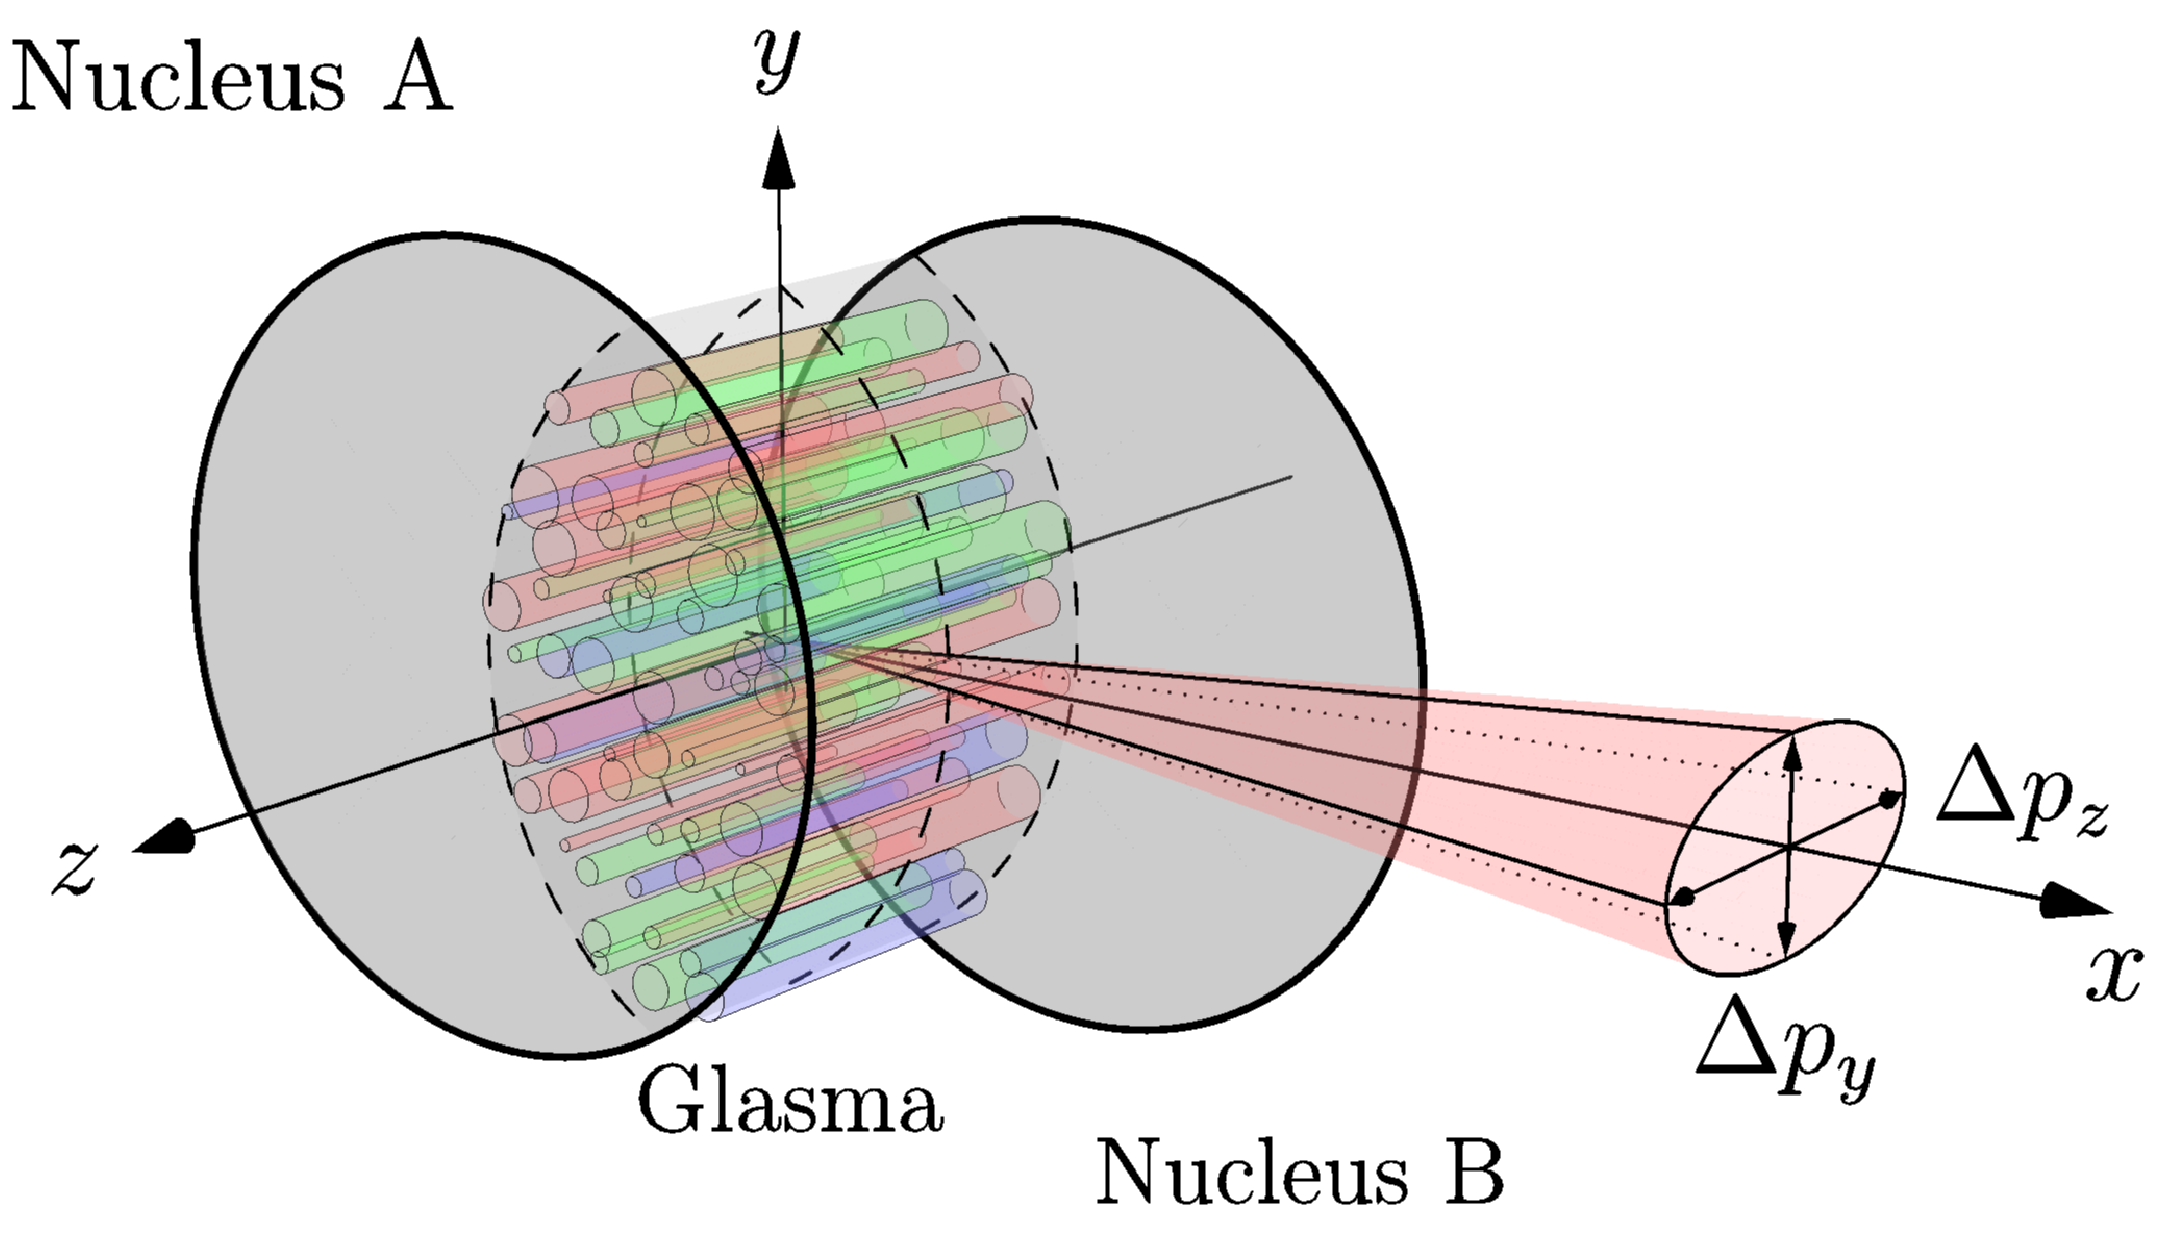
\includegraphics[height=0.7\paperheight]{images/momentum_broadening_flipped.pdf}}};
}
\setbeamertemplate{itemize item}{\raisebox{0.2em}{\scalebox{0.7}{${\color{normal}\blacktriangleright}$}}} 
\begin{frame}[plain,noframenumbering]{}
    \begin{center}
        \vspace{1cm}
        {\large\color{normal}Impact of glasma on hard probes}\\[0.3cm]
        {\huge\color{destacado}Transport coefficients}\\[0.3cm]
    \end{center}
\end{frame}
\setbeamertemplate{background}{}

%%%%%%%%%%%%%%%%%%%%%%%%%%%%%%%%%%%%%%%%%
%%%%%%%%%%%%%%%%% SLIDE %%%%%%%%%%%%%%%%%
%%%%%%%%%%%%%%%%%%%%%%%%%%%%%%%%%%%%%%%%%

\setbeamertemplate{background}{
\tikz[overlay,remember picture] \node[at=(current page.center), align=center] {\\[10pt]
{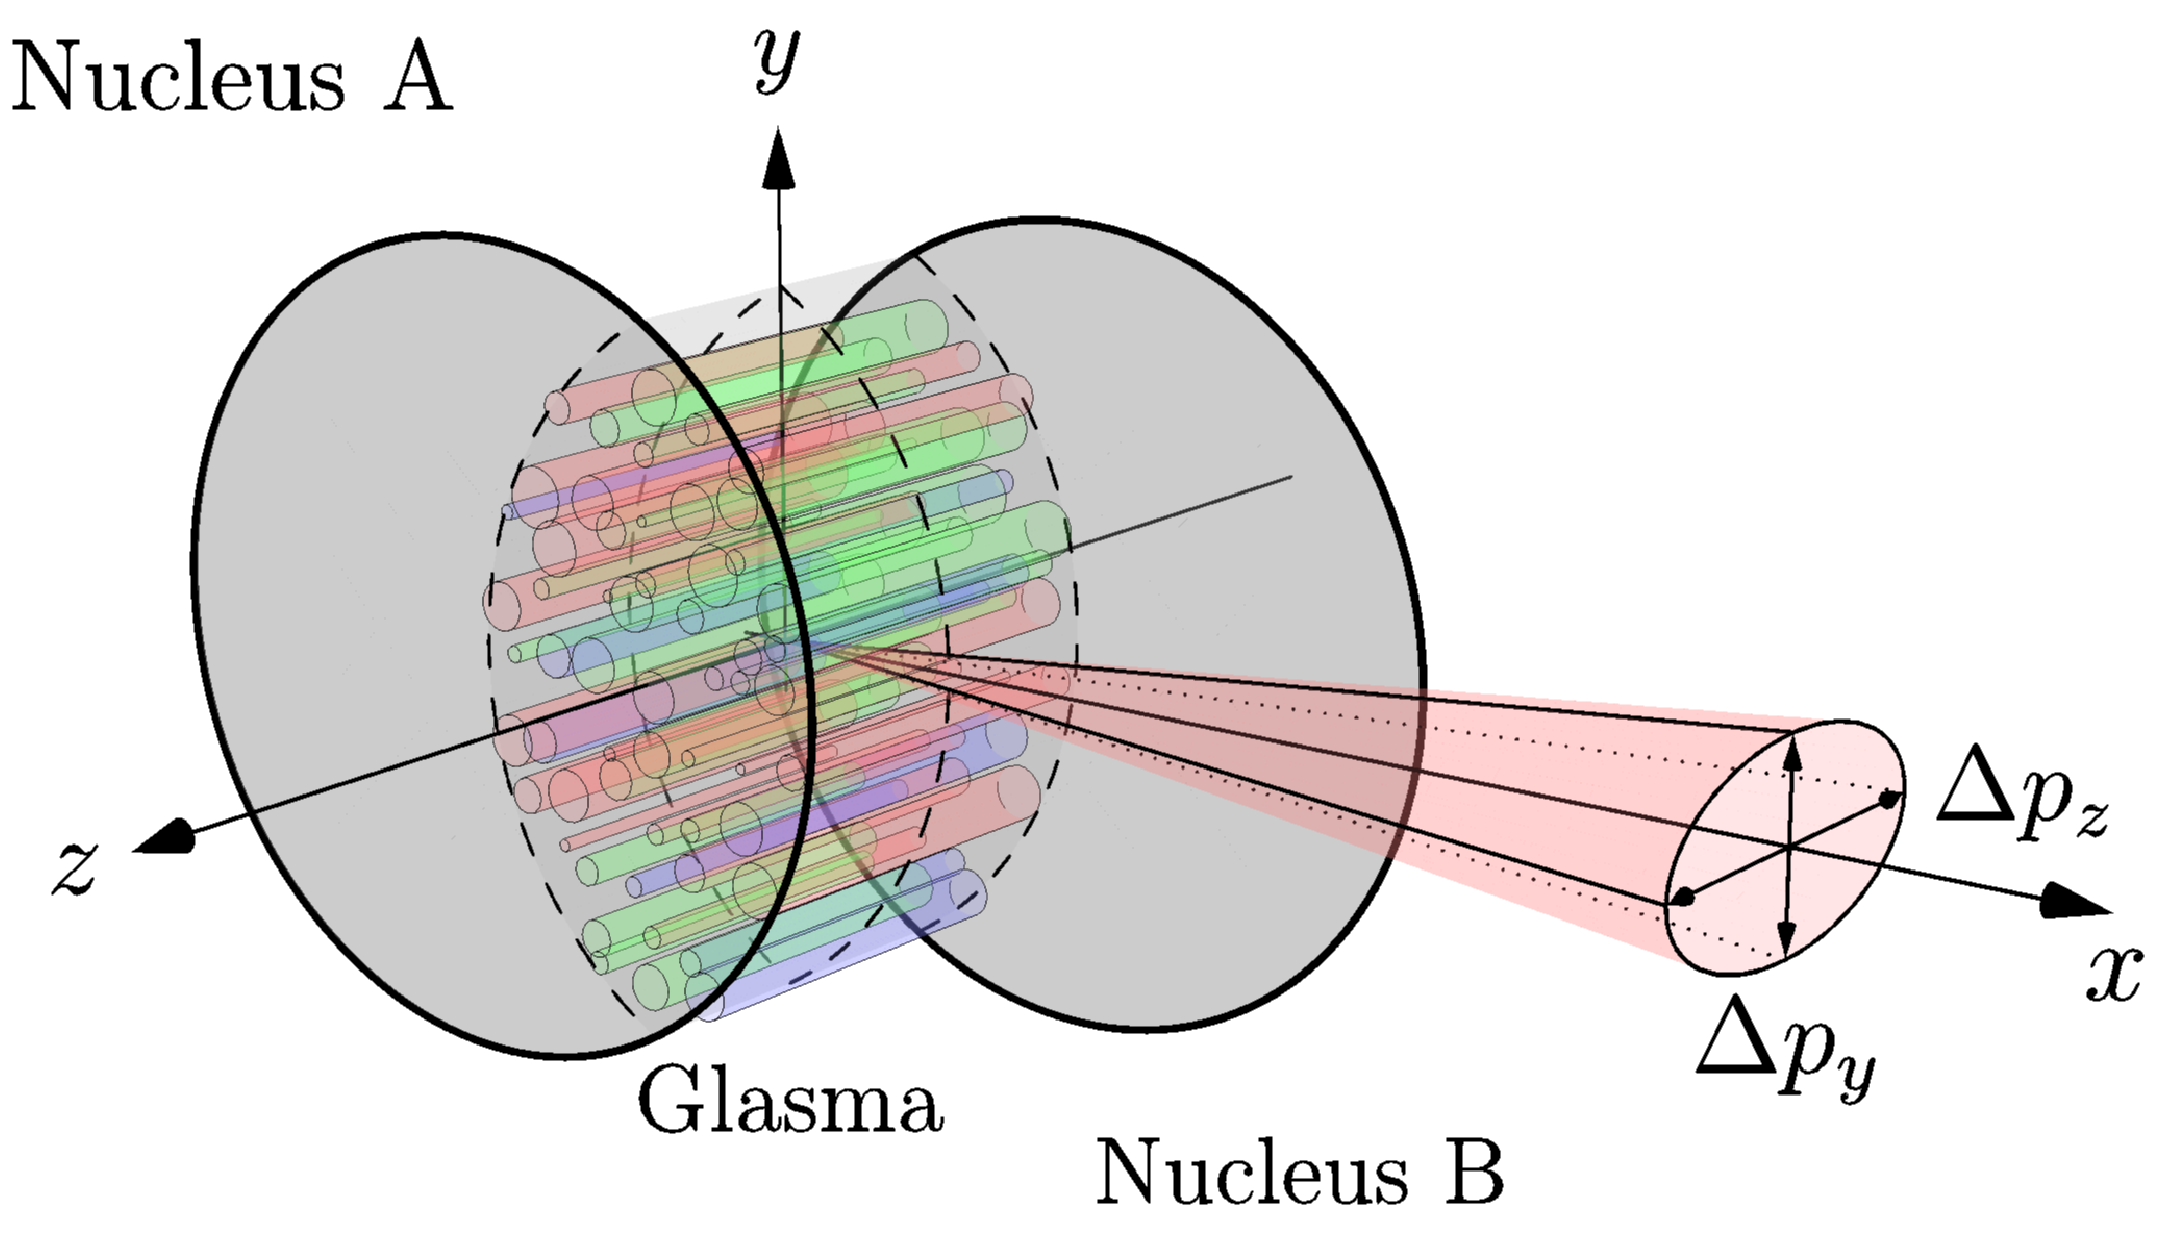
\includegraphics[height=0.7\paperheight]{images/momentum_broadening_flipped.pdf}}};
}
\setbeamertemplate{itemize item}{\raisebox{0.2em}{\scalebox{0.7}{${\color{normal}\blacktriangleright}$}}} 
\begin{frame}[plain,noframenumbering]{}
    \blfootnote{\scriptsize Ipp, Müller, Schuh \href{https://arxiv.org/abs/2009.14206}{{\color{customblue}\texttt{[2009.14206]}$^\text{\tiny\faExternalLink}$}}}
\end{frame}
\setbeamertemplate{background}{}

% %%%%%%%%%%%%%%%%%%%%%%%%%%%%%%%%%%%%%%%%%
% %%%%%%%%%%%%%%%%% SLIDE %%%%%%%%%%%%%%%%%
% %%%%%%%%%%%%%%%%%%%%%%%%%%%%%%%%%%%%%%%%%

\begin{frame}
    \frametitle{Transport coefficient $\kappa$}
    % \framesubtitle{Momentum broadening in glasma}
    \vspace{-10pt}
    \begin{columns}[onlytextwidth,t]
        \column{.033\textwidth}
        \column{.5\textwidth}

        \begin{figure}
            \centering
            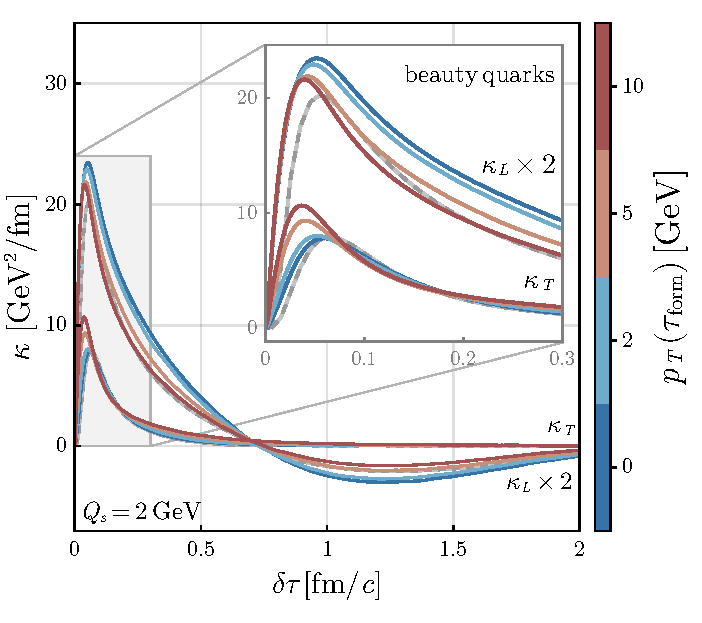
\includegraphics[width=0.9\textwidth]{images/hp23_mom_broad_kappa_anis_wong_vs_kappa-cropped.pdf}
        \end{figure}
       \column{.033\textwidth}
       \column{.4\textwidth}
        \begin{custombox2}{Classical transport}{lightgray}
            \small
            \begin{varwidth}{0.95\textwidth}
            \begin{itemize}\itemsep0em 
                \setbeamertemplate{itemize item}{\raisebox{0.2em}{\scalebox{0.7}{${\color{MidnightBlue}\blacktriangleright}$}}} 
                \item {\color{MidnightBlue}\bfseries Momentum broadening}\\ ${\color{MidnightBlue}\boldsymbol{\delta p^2_i}}(\tau)=p^2_i(\tau)-p^2_i(\tau_\mathrm{form})$
                \setbeamertemplate{itemize item}{\raisebox{0.2em}{\scalebox{0.7}{${\color{Maroon}\blacktriangleright}$}}} 
                \item {\color{Maroon}\bfseries Transport coefficient}\\ ${\color{Maroon}\boldsymbol{\kappa_i}}(\tau)=\dfrac{\mathrm{d}}{\mathrm{d}\tau}\langle{\color{MidnightBlue}\boldsymbol{\delta p^2_i}}(\tau)\rangle$ 
                \\[5pt]
                {\scriptsize\color{lightgray} Formation time $\tau_\mathrm{form}=1/2m$\\[1pt]
                Relative time $\delta\tau=\tau-\tau_\mathrm{form}$\\[-2pt]
                Longitudinal $i=L$, transverse $i=T$}
            \end{itemize}
            \end{varwidth}
        \end{custombox2}

        \begin{itemize}\itemsep0em 
            \footnotesize
            \setbeamertemplate{itemize item}{\raisebox{0.2em}{\scalebox{0.7}{${\color{lightgray}\blacktriangleright}$}}}
            {\color{lightgray}\item {\bfseries Anisotropic} $\kappa_L\neq\kappa_T$
            \item Rapid increase in $\kappa$ at early times 
            \item Negative $\kappa_L$ at late times}
            \setbeamertemplate{itemize item}{\raisebox{0.2em}{\scalebox{0.7}{${\color{palgold}\blacktriangleright}$}}} 
            \item {\bfseries\color{palgold}Large $\boldsymbol{\kappa}$ peak in glasma}
            \setbeamertemplate{itemize item}{\raisebox{0.2em}{\scalebox{0.7}{${\color{palviolet}\blacktriangleright}$}}}
            \item {\bfseries\color{palviolet}Approximate agreement with $\boldsymbol{\kappa}$ during EKT} {\color{lightgray}but not quantitative yet}
        \end{itemize}    
              
        \column{.033\textwidth}
    \end{columns}
    \vspace{-10pt}
    \blfootnote{\scriptsize Avramescu, Băran, Greco, Ipp, Müller, Ruggieri  \href{https://arxiv.org/abs/2307.07999}{{\color{palgold}\texttt{[2307.07999]}$^\text{\tiny\faExternalLink}$}}\\
    \hspace{16.5pt}Boguslavski, Kurkela, Lappi, Lindenbauer, Peuron \href{https://arxiv.org/abs/2303.12520}{{\color{palviolet}\texttt{[2303.12520]}$^\text{\tiny\faExternalLink}$}}
    }
\end{frame}

% %%%%%%%%%%%%%%%%%%%%%%%%%%%%%%%%%%%%%%%%%
% %%%%%%%%%%%%%%%%% SLIDE %%%%%%%%%%%%%%%%%
% %%%%%%%%%%%%%%%%%%%%%%%%%%%%%%%%%%%%%%%%%

\begin{frame}[noframenumbering]
    \frametitle{Transport coefficient $\kappa$}
    % \framesubtitle{Momentum broadening in glasma}
    % \vspace{-10pt}
    \begin{columns}[onlytextwidth,t]
        \column{.033\textwidth}
        \column{.5\textwidth}

        \begin{figure}
            \centering
            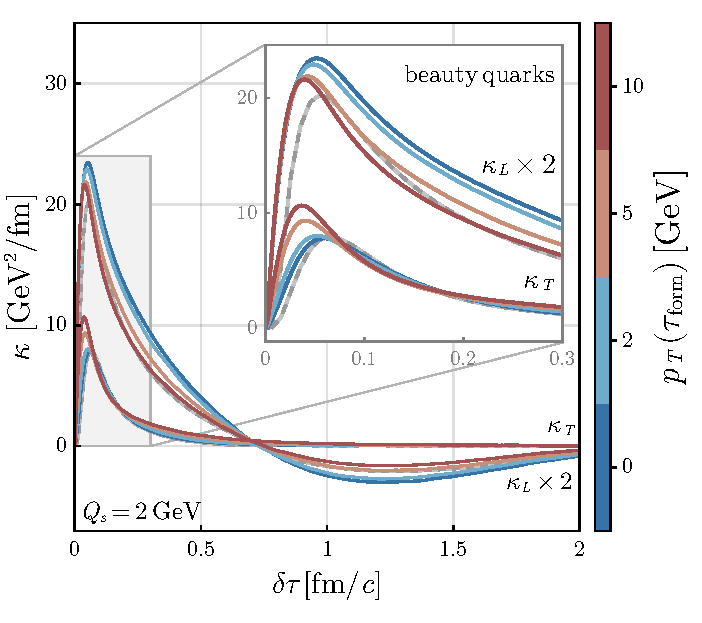
\includegraphics[width=0.9\textwidth]{images/hp23_mom_broad_kappa_anis_wong_vs_kappa-cropped.pdf}
        \end{figure}
       \column{.033\textwidth}
       \column{.4\textwidth}
       \begin{custombox2}{Classical transport}{lightgray}
        \small
        \begin{varwidth}{0.95\textwidth}
        \begin{itemize}\itemsep0em 
            \setbeamertemplate{itemize item}{\raisebox{0.2em}{\scalebox{0.7}{${\color{MidnightBlue}\blacktriangleright}$}}} 
            \item {\color{MidnightBlue}\bfseries Momentum broadening}\\ ${\color{MidnightBlue}\boldsymbol{\delta p^2_i}}(\tau)=p^2_i(\tau)-p^2_i(\tau_\mathrm{form})$
            \setbeamertemplate{itemize item}{\raisebox{0.2em}{\scalebox{0.7}{${\color{Maroon}\blacktriangleright}$}}} 
            \item {\color{Maroon}\bfseries Transport coefficient}\\ ${\color{Maroon}\boldsymbol{\kappa_i}}(\tau)=\dfrac{\mathrm{d}}{\mathrm{d}\tau}\langle{\color{MidnightBlue}\boldsymbol{\delta p^2_i}}(\tau)\rangle$ 
            \\[5pt]
            {\scriptsize\color{lightgray} Formation time $\tau_\mathrm{form}=1/2m$\\[1pt]
            Relative time $\delta\tau=\tau-\tau_\mathrm{form}$\\[-2pt]
            Longitudinal $i=L$, transverse $i=T$}
        \end{itemize}
        \end{varwidth}
    \end{custombox2}

        \begin{custombox2}{Limitation}{palgold}
            \small
            \begin{varwidth}{0.77\textwidth}
            \begin{itemize}\itemsep0em 
                \setbeamertemplate{itemize item}{\raisebox{0.2em}{\scalebox{0.7}{${\color{palgold}\blacktriangleright}$}}} 
                \item Transport coefficients $\neq$ {\color{palgold}\bfseries measurable} quantities
            \end{itemize}
            \end{varwidth}
        \end{custombox2} 
              
        \column{.033\textwidth}
    \end{columns}
    \blfootnote{\scriptsize Avramescu, Băran, Greco, Ipp, Müller, Ruggieri  \href{https://arxiv.org/abs/2307.07999}{{\color{palgold}\texttt{[2307.07999]}$^\text{\tiny\faExternalLink}$}}}
\end{frame}




%%%%%%%%%%%%%%%%%%%%%%%%%%%%%%%%%%%%%%%%%
%%%%%%%%%%%%%% SUBSECTION %%%%%%%%%%%%%%%
%%%%%%%%%%%%%%%%%%%%%%%%%%%%%%%%%%%%%%%%%

% \subsection{Field correlators}

%%%%%%%%%%%%%%%%%%%%%%%%%%%%%%%%%%%%%%%%%
%%%%%%%%%%%%%%%%% SLIDE %%%%%%%%%%%%%%%%%
%%%%%%%%%%%%%%%%%%%%%%%%%%%%%%%%%%%%%%%%%

\begin{frame}
    \frametitle{Field correlators}
    % \framesubtitle{Limiting cases}
        \begin{center}
            \begin{custombox2}{Gauge invariant force correlator}{lightgray}
                \small
                \begin{varwidth}{0.78\textwidth}
                \begin{itemize}\itemsep0em 
                    \setbeamertemplate{itemize item}{\raisebox{0.2em}{\scalebox{0.7}{${\color{lightgray}\blacktriangleright}$}}} 
                    \item \begin{center} Momentum broadening for known trajectories from {\color{palteal}\bfseries force correlator}\\[5pt]
                    $\displaystyle\langle \delta p^2_i(\tau)\rangle= g^2 \int_{\tau_\mathrm{form}}^{\tau}\mathrm{d}\tau^{\prime}\int_{\tau_\mathrm{form}}^{\tau}\mathrm{d}\tau^{\prime\prime}{\color{palteal}\boldsymbol{\Big\langle \mathrm{Tr}\big[\widetilde{\mathcal{F}}_i(\tau^{\prime})\widetilde{\mathcal{F}}_i(\tau^{\prime\prime})\big]\Big\rangle}}$\\[5pt]
                    {\scriptsize\color{lightgray} Lorentz force $\mathcal{F}_i=F_{i\mu}p^\mu/p^0$, gauge invariant $\widetilde{\mathcal{F}}_i$ parallel transported on lattice}
                    \end{center} 
                \end{itemize}
                \end{varwidth}
            \end{custombox2}
        
           \end{center} 

        \begin{columns}
            \begin{column}{0.033\textwidth}\end{column}
            \begin{column}{0.4\textwidth}
                \centering
                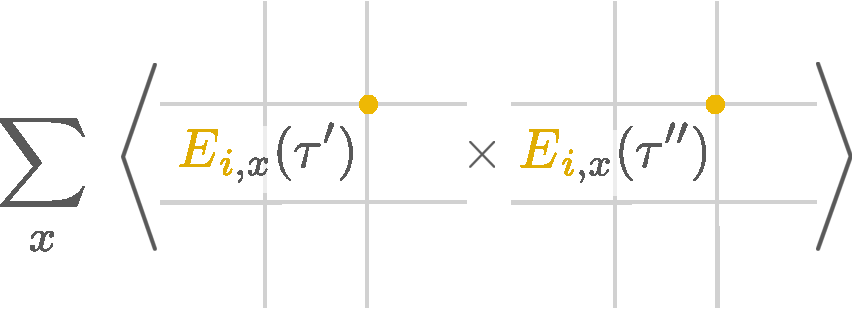
\includegraphics[width=0.9\columnwidth]{images/corr_hqs.pdf}
            \end{column}
            \begin{column}{0.01\textwidth}\end{column}
            \begin{column}{0.5\textwidth}
                % \centering
                \vspace{-10pt}
                \setbeamertemplate{itemize item}{\raisebox{0.2em}{\scalebox{0.7}{${\color{customyellow}\blacktriangleright}$}}} 
                \begin{itemize}
                    \item {\color{customyellow} Static heavy quarks} with $m\rightarrow\infty$
                \end{itemize} 
                \vspace{7pt}
                {\footnotesize
                \begin{equation*}
                    \hspace{10pt}\langle \delta p^2_i\rangle\big|_{\color{customyellow}m\rightarrow\infty}\propto \int\mathrm{d}\tau^{\prime}\int\mathrm{d}\tau^{\prime\prime}\Big\langle \mathrm{Tr}\big[{\color{customyellow}E_i}(\tau^{\prime}){\color{customyellow}E_i}(\tau^{\prime\prime})\big]\Big\rangle
                \end{equation*}}
            \end{column}
            \begin{column}{0.056\textwidth}\end{column}
        \end{columns}

        \begin{columns}
            \begin{column}{0.033\textwidth}\end{column}
            \begin{column}{0.4\textwidth}
                \centering
                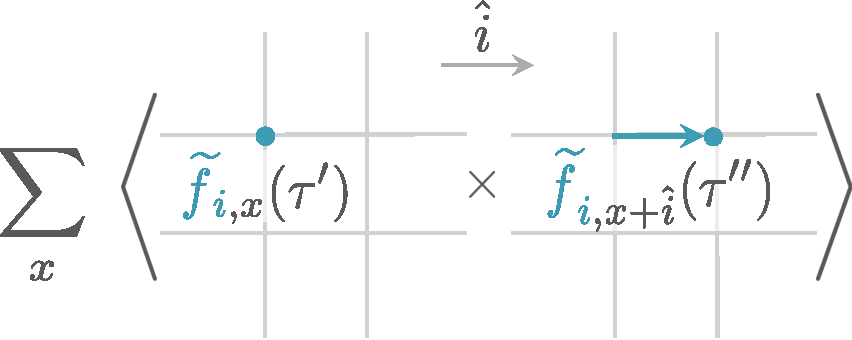
\includegraphics[width=0.9\columnwidth]{images/corr_jets.pdf}
            \end{column}
            \begin{column}{0.01\textwidth}\end{column}
            \begin{column}{0.5\textwidth}
                % \centering
                \vspace{-10pt}
                \setbeamertemplate{itemize item}{\raisebox{0.2em}{\scalebox{0.7}{${\color{customblue}\blacktriangleright}$}}} 
                \begin{itemize}
                    \item {\color{customblue} Eikonal jets} with $p^x\rightarrow\infty$
                \end{itemize} 
                \vspace{7pt}
                {\footnotesize
                \begin{equation*}
                    \hspace{10pt}\langle \delta p^2_i\rangle\big|_{\color{customblue}p^x\rightarrow\infty}\propto \int\mathrm{d}\tau^{\prime}\int\mathrm{d}\tau^{\prime\prime}\Big\langle \mathrm{Tr}\big[{\color{customblue}\widetilde{f}_i}(\tau^{\prime}){\color{customblue}\widetilde{f}_i}(\tau^{\prime\prime})\big]\Big\rangle
                \end{equation*}}
                {\scriptsize\color{lightgray} \hspace{18pt}$f_y=E_y-B_z$, $f_z=E_z+B_y$}
            \end{column}
            \begin{column}{0.056\textwidth}\end{column}
        \end{columns}
\end{frame}



%%%%%%%%%%%%%%%%%%%%%%%%%%%%%%%%%%%%%%%%%
%%%%%%%%%%%%%% SUBSECTION %%%%%%%%%%%%%%%
%%%%%%%%%%%%%%%%%%%%%%%%%%%%%%%%%%%%%%%%%

\subsection{Observables}

%%%%%%%%%%%%%%%%%%%%%%%%%%%%%%%%%%%%%%%%%
%%%%%%%%%%%%%%%%% SLIDE %%%%%%%%%%%%%%%%%
%%%%%%%%%%%%%%%%%%%%%%%%%%%%%%%%%%%%%%%%%

\begin{frame}
    \frametitle{Phenomenology}
\end{frame}

%%%%%%%%%%%%%%%%%%%%%%%%%%%%%%%%%%%%%%%%%
%%%%%%%%%%%%%%%% SECTION %%%%%%%%%%%%%%%%
%%%%%%%%%%%%%%%%%%%%%%%%%%%%%%%%%%%%%%%%%

\section{Open questions}

%%%%%%%%%%%%%%%%%%%%%%%%%%%%%%%%%%%%%%%%%
%%%%%%%%%%%%%% SUBSECTION %%%%%%%%%%%%%%%
%%%%%%%%%%%%%%%%%%%%%%%%%%%%%%%%%%%%%%%%%

%%%%%%%%%%%%%%%%%%%%%%%%%%%%%%%%%%%%%%%%%
%%%%%%%%%%%%%%%%% SLIDE %%%%%%%%%%%%%%%%%
%%%%%%%%%%%%%%%%%%%%%%%%%%%%%%%%%%%%%%%%%

\begin{frame}
    \frametitle{Open questions}
\end{frame}






\end{document}